\documentclass{hcmut-report}
\usepackage{tabularx}
\usepackage{longtable}
\usepackage{multirow}
\usepackage{array}
\usepackage{float}
\usepackage{listings}
\usepackage{xcolor}
\usepackage{etoolbox}
\AtBeginEnvironment{table}{\singlespacing}

% --- Overflow prevention & clean full-grid table spacing ---
\sloppy
\emergencystretch=3em
\renewcommand{\arraystretch}{1.24}
\setlength{\tabcolsep}{4.5pt}
\newcolumntype{Y}{>{\raggedright\arraybackslash}X}
\newcolumntype{P}[1]{>{\raggedright\arraybackslash}p{#1}}
\newcolumntype{C}[1]{>{\centering\arraybackslash}p{#1}}
\newcolumntype{R}[1]{>{\raggedleft\arraybackslash}p{#1}}

% --- Clean ASCII source code listing configuration ---
\definecolor{codebg}{RGB}{248,249,250}
\definecolor{codeframe}{RGB}{180,180,180}
\definecolor{codekw}{RGB}{0,92,197}
\definecolor{codecmt}{RGB}{34,134,58}
\definecolor{codestr}{RGB}{215,58,73}

\lstset{
  backgroundcolor=\color{codebg},
  frame=single,
  rulecolor=\color{codeframe},
  basicstyle=\footnotesize\ttfamily,
  keywordstyle=\color{codekw}\bfseries,
  commentstyle=\color{codecmt}\itshape,
  stringstyle=\color{codestr},
  numbers=left,
  numberstyle=\tiny\color{gray},
  numbersep=5pt,
  xleftmargin=12pt,
  xrightmargin=4pt,
  breaklines=true,
  breakatwhitespace=false,
  showstringspaces=false,
  tabsize=2,
  captionpos=b
}

% --- Cover Page Metadata (HCMUT - Faculty of Computer Science & Engineering) ---
\deptname{Faculty of Computer Science and Engineering}
\labname{}
\shortlabname{IoT -- HK261}
\coursename{Internet of Things (IoT) -- Semester HK261}
\reporttype{COURSE PROJECT REPORT}
\title{\LARGE\bfseries PRIVACY-PRESERVING DEVICE-FREE INDOOR FALL AND INTRUSION\\[4pt]\LARGE\bfseries DETECTION SYSTEM USING WI-FI CSI, BLE, AND EDGE-GPU AI}
\advisorlabel{Instructor}
\advisor{& Dr. Nguyễn Hòa Hưng}
\studentlabel{Group Members}
\stuname{%
  & Lê Ngọc Uy Phong & (Student ID: 2352905) \\
  & Huỳnh Võ Quỳnh Anh & (Student ID: 2452043) \\
  & Trần Thị Bình & (Student ID: 2452157)
}
\reportplace{Ho Chi Minh City}
\reporttime{November 2026}

\begin{document}

\coverpage

% =========================================================================
% FRONT MATTER: SUBMISSION INFO, TASK ASSIGNMENT & TECH RUBRIC ASSESSMENT
% =========================================================================
\section*{Submission Information and Group Roster}
\addcontentsline{toc}{section}{Submission Information and Group Roster}

\begin{table}[H]
\centering
\caption{Group Member Roster for the IoT Course Project (Semester HK261)}
\label{tab:group_roster}
\small
\begin{tabularx}{\textwidth}{|C{0.9cm}|P{4.6cm}|C{2.4cm}|Y|}
\hline
\textbf{No.} & \textbf{Full Name} & \textbf{Student ID} & \textbf{Institutional Email \& Primary Role} \\
\hline
1 & Lê Ngọc Uy Phong & 2352905 & \texttt{phong.le9999\allowbreak @hcmut.edu.vn} -- Hardware, ESP-NOW CSI, BLE, Web UI \\
\hline
2 & Huỳnh Võ Quỳnh Anh & 2452043 & \texttt{anh.huynhvo02\allowbreak @hcmut.edu.vn} -- Digital DSP, INT8 TinyML, GPU 2D-CNN \\
\hline
3 & Trần Thị Bình & 2452157 & \texttt{binh.tranbinh2856\allowbreak @hcmut.edu.vn} -- PC Gateway, CoreIOT Sync, RuleChain, OTA \\
\hline
\end{tabularx}
\end{table}

\begin{table}[H]
\centering
\caption{Project Deliverable Summary and Submission Links}
\label{tab:submission_info}
\small
\begin{tabularx}{\textwidth}{|P{4.3cm}|Y|}
\hline
\textbf{Deliverable Item} & \textbf{Specification / Access Path} \\
\hline
Project Title (English) & Privacy-Preserving Device-Free Indoor Fall and Intrusion Detection System using Wi-Fi CSI, BLE, and Collaborative Edge-GPU AI \\
\hline
Course \& Instructor & Internet of Things (Semester HK261, AY 2026--2027) -- Dr. Nguyễn Hòa Hưng (\texttt{nguyenhoahung@hcmut.edu.vn}) \\
\hline
Report File Name & \texttt{HK261\_Group01\_IoTReport.pdf} (compiled from \texttt{HK261\_Group01\_IoTReport.tex}) \\
\hline
Source Code Repository & \texttt{https://github.com/\allowbreak hcmut-iot-hk261/\allowbreak wifi-csi-fall-detection} \\
\hline
Demonstration Video & \texttt{https://youtu.be/\allowbreak [Update-Demo-Video-ID-Before-LMS-Upload]} (5--10 minutes) \\
\hline
CoreIOT Live Dashboard & \texttt{https://app.coreiot.io/\allowbreak dashboard/\allowbreak [Update-Public-Dashboard-UUID]} \\
\hline
\end{tabularx}
\end{table}

\section*{Member Task Assignment Table}
\addcontentsline{toc}{section}{Member Task Assignment Table}

\begin{table}[H]
\centering
\caption{Detailed Work Breakdown and Contribution Ratios Across Group Members}
\label{tab:task_assignment}
\small
\begin{tabularx}{\textwidth}{|P{3.3cm}|Y|P{2.8cm}|C{1.5cm}|}
\hline
\textbf{Member} & \textbf{Assigned Engineering Modules and Deliverables} & \textbf{Tech Codes} & \textbf{Weight} \\
\hline
Lê Ngọc Uy Phong\newline (ID: 2352905) & Designed hardware schematics and GPIO pin maps for both YoloUNO ESP32-S3 boards; implemented 100~Hz ESP-NOW CSI Tx/Rx firmware, I2C DHT20 driver with Tasmota configuration, time-sliced BLE 5.0 passive scanner, and Node~2 Embedded HTTP Web Server; compiled PlatformIO binaries. & \texttt{T01}, \texttt{T03}, \texttt{T06}, \texttt{T07}, \texttt{T14} & 34\% \\
\hline
Huỳnh Võ Quỳnh Anh\newline (ID: 2452043) & Formulated the 64-subcarrier OFDM multipath physics model; implemented causal Hampel and 4th-order Butterworth DSP filters; built CSV data recorder; trained and quantized the 3.3~KB INT8 1D-CNN TinyML model and 382.5~KB RTX~5070 ONNX 2D-CNN; ran 950-window quantitative evaluations. & \texttt{T04}, \texttt{T05}, \texttt{T09}, \texttt{N04} & 33\% \\
\hline
Trần Thị Bình\newline (ID: 2452157) & Built the multi-threaded PC Local IoT Gateway and Hardware-in-the-Loop (HIL) cluster simulator; authored the Streamlit real-time CSI Heatmap and automatic event-snapshot dashboard; integrated CoreIOT Gateway MQTT sync, smart RuleChain JSON, Telegram Bot alerts, and Dual-OTA updater. & \texttt{T08}, \texttt{T10}, \texttt{T11}, \texttt{T12}, \texttt{T13}, \texttt{T14}, \texttt{T15}, \texttt{N06}, \texttt{N01} & 33\% \\
\hline
\multicolumn{3}{|r|}{\textbf{Total Group Contribution}} & \textbf{100\%} \\
\hline
\end{tabularx}
\end{table}

\newpage
\section*{Technology Element Self-Assessment Tables}
\addcontentsline{toc}{section}{Technology Element Self-Assessment Tables}

In accordance with the official IoT Course Project rubric, Table~\ref{tab:rubric_t} summarizes our implementation status across all 15 standard technology elements (\texttt{T01}--\texttt{T15}, capped at \textbf{8.0 points}), and Table~\ref{tab:rubric_n} summarizes our bonus elements (\texttt{N01}--\texttt{N07}, capped at \textbf{1.0 point}).

\begin{table}[H]
\centering
\caption{Table A -- Self-Assessment of Standard Technology Elements (\texttt{T01}--\texttt{T15})}
\label{tab:rubric_t}
\footnotesize
\renewcommand{\arraystretch}{1.14}
\begin{tabularx}{\textwidth}{|C{0.9cm}|P{4.1cm}|C{0.9cm}|C{1.35cm}|Y|}
\hline
\textbf{Code} & \textbf{Technology Element} & \textbf{Max} & \textbf{Claim} & \textbf{Implemented Source File \& Report Section} \\
\hline
\texttt{T01} & Basic I2C Sensor (Tasmota / ESP) & 0.5 & 0.5 & \texttt{firmware/\allowbreak node1\_tx\_env/\allowbreak src/\allowbreak main.cpp} \& Tasmota rule (Sec.~3.2.1) \\
\hline
\texttt{T02} & Modbus RS485 Industrial Sensor & 1.0 & 0.0 & Not used (residential healthcare scope uses I2C + RF CSI) \\
\hline
\texttt{T03} & BLE Communication \& Identity Scan & 1.5 & 1.5 & \texttt{firmware/\allowbreak node2\_rx\_edge\_ai/\allowbreak include/\allowbreak ble\_scanner.h} (Sec.~3.2.2, 3.3) \\
\hline
\texttt{T04} & On-Device TinyML Inference & 1.0 & 1.0 & \texttt{tinyml\_infer.h} + \texttt{model\_data.h} (3.3~KB INT8 1D-CNN, Sec.~3.5.3) \\
\hline
\texttt{T05} & Custom CSV Dataset \& TinyML Train & 1.0 & 1.0 & \texttt{ai\_training/\allowbreak csi\_serial\_collector.py}, \texttt{train\_tinyml\_1dcnn.py} (Sec.~3.5) \\
\hline
\texttt{T06} & ESP-NOW Wireless Link (100~Hz CSI) & 1.5 & 1.5 & \texttt{firmware/\allowbreak include/\allowbreak csi\_protocol.h}, 24B CRC-8 frame (Sec.~3.3) \\
\hline
\texttt{T07} & Custom Embedded Web Server & 1.0 & 1.0 & \texttt{firmware/\allowbreak node2\_rx\_edge\_ai/\allowbreak include/\allowbreak web\_server.h} (Sec.~3.2.3) \\
\hline
\texttt{T08} & Local IoT Gateway Data \& RPC Router & 1.0 & 1.0 & \texttt{gateway/\allowbreak main\_gateway.py} (\texttt{LocalIoTGatewayService}, Sec.~3.4) \\
\hline
\texttt{T09} & AI Model Running on Local Gateway & 1.0 & 1.0 & \texttt{gateway/\allowbreak gpu\_spectrogram\_ai.py} (STFT 2D-CNN, Sec.~3.5.2) \\
\hline
\texttt{T10} & Local Gateway Monitoring \& Ctrl UI & 1.0 & 1.0 & \texttt{gateway/\allowbreak streamlit\_ui.py} (Live CSI Heatmap + RPC, Sec.~3.4) \\
\hline
\texttt{T11} & CoreIOT Device Profile \& Dashboard & 1.0 & 1.0 & \texttt{coreiot/\allowbreak dashboard\_template.json} (Sec.~3.6.1) \\
\hline
\texttt{T12} & Smart Processing on RuleChain & 1.0 & 1.0 & \texttt{coreiot/\allowbreak rulechain\_fall\_sec.json} (7-node graph, Sec.~3.6.2) \\
\hline
\texttt{T13} & Emergency Alert Push (Telegram Bot) & 0.5 & 0.5 & \texttt{gateway/\allowbreak coreiot\_sync.py} (\texttt{TelegramAlertClient}, Sec.~3.6.2) \\
\hline
\texttt{T14} & Remote OTA Firmware Update & 2.0 & 2.0 & \texttt{firmware/\allowbreak include/\allowbreak ota\_updater.h} + SHA-256 rollback (Sec.~3.6.3) \\
\hline
\texttt{T15} & CoreIOT Gateway -- Local Sync & 2.0 & 2.0 & \texttt{gateway/\allowbreak coreiot\_sync.py} (\texttt{v1/gateway/*} API, Sec.~3.6.1) \\
\hline
\multicolumn{2}{|r|}{\textbf{Raw Sum / Rubric Cap (Table A)}} & \textbf{16.0} & \textbf{8.0 / 8.0} & \textbf{14.0 raw points verified; capped at maximum 8.0 pts} \\
\hline
\end{tabularx}
\end{table}

\begin{table}[H]
\centering
\caption{Table B -- Self-Assessment of Advanced / Bonus Elements (\texttt{N01}--\texttt{N07})}
\label{tab:rubric_n}
\footnotesize
\renewcommand{\arraystretch}{1.14}
\begin{tabularx}{\textwidth}{|C{0.9cm}|P{4.2cm}|C{0.9cm}|C{1.35cm}|Y|}
\hline
\textbf{Code} & \textbf{Advanced Technology Element} & \textbf{Max} & \textbf{Claim} & \textbf{Implemented Source File \& Verification Evidence} \\
\hline
\texttt{N04} & GPU-Accelerated Gateway AI Inference & +1.0 & +1.0 & \texttt{ONNX Runtime 1.23.2} \texttt{CUDAExecutionProvider} on \textbf{NVIDIA GeForce RTX~5070 Laptop GPU} (0.313~ms single, 0.030~ms batch-16; Sec.~3.5.3, 3.7) \\
\hline
\texttt{N06} & Custom Auto Event-Detecting \& Snapshot-Recording Dashboard & +1.0 & +1.0 & Automatic Hampel-peak localization, dual-panel CSI + STFT PNG capture, and searchable event gallery in \texttt{main\_gateway.py} \& \texttt{streamlit\_ui.py} (Sec.~3.7) \\
\hline
\texttt{N01} & Natural-Language Telemetry Log Assistant (Backup Bonus) & +1.0 & Backup & Built-in interactive Q\&A tab querying \texttt{event\_snapshots\_log.jsonl} inside \texttt{gateway/\allowbreak streamlit\_ui.py} (Sec.~3.7) \\
\hline
\multicolumn{2}{|r|}{\textbf{Raw Sum / Rubric Cap (Table B)}} & \textbf{3.0} & \textbf{1.0 / 1.0} & \textbf{2.0+ raw bonus points verified; capped at maximum 1.0 pt} \\
\hline
\end{tabularx}
\end{table}

\newpage
\tableofcontents
\newpage

\section*{List of Abbreviations}
\addcontentsline{toc}{section}{List of Abbreviations}
\vspace{-0.3cm}
\begin{table}[H]
\centering
\caption{Key Technical Acronyms Used Throughout This Report}
\label{tab:abbreviations}
\footnotesize
\renewcommand{\arraystretch}{1.00}
\begin{tabularx}{\textwidth}{|P{2.4cm}|P{5.5cm}|Y|}
\hline
\textbf{Acronym} & \textbf{Full Term} & \textbf{Technical Meaning in This Project} \\
\hline
BLE & Bluetooth Low Energy & Short-range 2.4~GHz beacon protocol used for passive resident identity verification (\texttt{T03}). \\
\hline
CNN & Convolutional Neural Network & Deep learning architecture used in 1D form on ESP32-S3 (\texttt{T04}) and 2D form on the PC GPU (\texttt{T09}). \\
\hline
CSI & Channel State Information & Complex amplitude and phase matrix across 64 OFDM subcarriers extracted from the Wi-Fi PHY layer. \\
\hline
CUDA & Compute Unified Device Architecture & NVIDIA parallel GPU execution platform accelerating ONNX Runtime on the RTX~5070 (\texttt{N04}). \\
\hline
ESP-NOW & Espressif Connectionless Wi-Fi Protocol & Low-overhead MAC-layer protocol streaming 100~Hz CSI probe frames without an access point (\texttt{T06}). \\
\hline
HIL & Hardware-in-the-Loop & Dual-mode execution design allowing identical Gateway/Cloud code to run on physical MCUs or physics simulation. \\
\hline
INT8 & 8-Bit Signed Integer Quantization & Symmetric weight/activation compression shrinking our Edge 1D-CNN to 3,392~bytes (\texttt{T04}). \\
\hline
LLTF & Legacy Long Training Field & IEEE 802.11n preamble symbol used by the ESP32-S3 baseband to estimate channel frequency response. \\
\hline
LOS / NLOS & Line-of-Sight / Non-Line-of-Sight & Direct unobstructed propagation vs.\ through-wall / occluded indoor RF propagation paths. \\
\hline
MAD & Median Absolute Deviation & Robust dispersion estimator inside our causal Hampel filter to reject impulsive AGC spikes. \\
\hline
MQTT & Message Queuing Telemetry Transport & Publish/subscribe broker protocol synchronizing the PC Gateway with CoreIOT Cloud (\texttt{T15}). \\
\hline
OFDM & Orthogonal Frequency-Division Multiplexing & Multi-carrier modulation dividing a 20~MHz Wi-Fi channel into 52 active data/pilot subcarriers. \\
\hline
ONNX & Open Neural Network Exchange & Portable graph format executing our 2D-CNN on \texttt{CUDAExecutionProvider} (\texttt{N04}). \\
\hline
OTA & Over-The-Air Firmware Update & Remote binary delivery with SHA-256 verification and dual-slot \texttt{ota\_0}/\texttt{ota\_1} rollback (\texttt{T14}). \\
\hline
RPC & Remote Procedure Call & Downlink command mechanism from CoreIOT or Local UI to Node~2 actuators and thresholds (\texttt{T08}). \\
\hline
STFT & Short-Time Fourier Transform & Time-frequency transform converting 2.0~s CSI windows into $3\times 64\times 64$ Doppler spectrograms. \\
\hline
\end{tabularx}
\end{table}

\newpage
% =========================================================================
% CHAPTER 1. INTRODUCTION
% =========================================================================
\section[Introduction]{Introduction}
\label{sec:intro}

\subsection[Problem Statement]{Problem Statement}
\label{sec:problem}

Unintentional falls represent one of the leading causes of injury-related hospitalization and mortality among older adults living independently. According to global public health reports from the World Health Organization (WHO), approximately 28\%--35\% of individuals aged 65 and older experience at least one fall each year, and more than 684,000 fatal falls occur worldwide annually~\cite{who_falls}. Crucially, clinical studies show that the medical outcome of an indoor fall depends heavily on response latency: when an elderly person remains immobilized on the floor for over one hour (known as a ``long-lie'' episode), mortality within six months rises sharply due to dehydration, hypothermia, rhabdomyolysis, and pneumonia.

Despite decades of research, deploying a practical indoor fall and home-security monitoring system in real bedrooms and bathrooms remains hindered by three fundamental engineering barriers:
\begin{enumerate}
  \item \textbf{Severe Privacy Invasion of Camera-Based Vision Systems:} Optical RGB and depth cameras paired with pose-estimation neural networks achieve high accuracy under bright illumination, but elderly residents overwhelmingly reject cameras inside private living spaces such as bedrooms and bathrooms~\cite{wang_wifi_fall}. Optical cameras also degrade in complete darkness or behind shower curtains and furniture.
  \item \textbf{Poor User Compliance of Wearable Inertial Sensors:} Wristbands, smartwatches, and neck pendants containing 3-axis accelerometers and gyroscopes require the user to wear and recharge the device every day~\cite{mubashir_survey}. In practice, elderly individuals frequently forget to put wearables back on at night or remove them before entering the bathroom---precisely where slip-and-fall accidents are most prevalent.
  \item \textbf{Identity Blindness and False Alarms in Naive RF Motion Sensors:} Device-free radio-frequency (RF) sensing using Wi-Fi Channel State Information (CSI)~\cite{halperin_csitool,yousefi_survey} can sense human motion through darkness and thin partitions without requiring wearables or cameras. However, existing single-tier Wi-Fi CSI prototypes suffer from two major flaws: (i) lightweight threshold rules confuse rapid daily movements (such as sitting down quickly onto a chair) with true falls, and (ii) pure CSI motion detectors cannot tell whether a walking person in an armed house is a family member returning home or an unauthorized intruder.
\end{enumerate}

To solve all three challenges simultaneously, this project designs, implements, and quantitatively validates a \textbf{Privacy-Preserving Device-Free Indoor Fall and Intrusion Detection System} built on two low-cost \textbf{YoloUNO (ESP32-S3)} microcontrollers~\cite{espressif_csi}, passive \textbf{Bluetooth Low Energy (BLE)} identity tags, a \textbf{Two-Tier Collaborative Edge-GPU AI pipeline}, and end-to-end \textbf{CoreIOT Cloud} automation.

\subsection[Related Solutions]{Related Solutions and Research Gap}
\label{sec:related}

Table~\ref{tab:related_work} compares four mainstream categories of indoor fall and intrusion monitoring technologies against our proposed system across privacy preservation, user convenience, dark/occluded operation, identity awareness, and hardware cost.

\begin{table}[H]
\centering
\caption{Comparison of Existing Fall and Indoor Security Solutions vs.\ Proposed System}
\label{tab:related_work}
\footnotesize
\begin{tabularx}{\textwidth}{|P{2.5cm}|P{1.75cm}|P{1.95cm}|P{1.9cm}|P{1.95cm}|Y|}
\hline
\textbf{Approach} & \textbf{Privacy Safe?} & \textbf{Device-Free?} & \textbf{Works in Dark / NLOS?} & \textbf{Resident vs.\ Intruder?} & \textbf{Key Practical Limitation} \\
\hline
Wearable IMU Pendant / Watch~\cite{mubashir_survey} & Yes & No (Must wear) & Yes & Self-only & Forgotten during night/shower; battery depletion disables protection. \\
\hline
RGB / Depth AI Camera & No (Video leak risk) & Yes & Poor in dark / occluded & Via facial recognition & Unacceptable in bathrooms and bedrooms; blocked by furniture. \\
\hline
60~GHz FMCW mmWave Radar & Yes & Yes & Moderate (LOS mostly) & No native ID & Expensive dedicated radar modules (\$45--\$120/room); high wall attenuation. \\
\hline
Single-Tier Wi-Fi CSI~\cite{wang_wifi_fall,zhang_widar} & Yes & Yes & Yes (2.4~GHz diffraction) & No & High false-positive rate on rapid sitting; relies on single MCU or offline PC. \\
\hline
\textbf{Proposed System (Wi-Fi CSI + BLE + 2-Tier AI)} & \textbf{Yes (Zero camera)} & \textbf{Yes (Fall is 100\% passive)} & \textbf{Yes (LOS \& NLOS)} & \textbf{Yes (BLE MAC + RSSI)} & \textbf{Low cost (\textasciitilde\$22 hardware), offline-safe Edge INT8 + RTX~5070 GPU verification.} \\
\hline
\end{tabularx}
\end{table}

As highlighted in Table~\ref{tab:related_work}, our architecture bridges the gap between low-cost microcontroller sensing and high-precision spectrogram deep learning:
\begin{itemize}
  \item \textbf{100\% Device-Free Fall Safety + Zero-Touch BLE Security:} Elderly fall detection requires zero worn devices (even if a resident leaves their phone on a desk, a fall is immediately flagged as a critical medical emergency). Meanwhile, passive BLE MAC whitelist and RSSI scanning (\texttt{T03}) suppresses false security alarms when family members walk indoors while catching unauthenticated intruders.
  \item \textbf{Two-Tier Collaborative Edge-GPU AI:} Tier~1 runs an ultra-compact \textbf{3.3~KB INT8 1D-CNN} directly on Node~2's ESP32-S3 (\texttt{T04}) so local buzzer/LED alarms fire within milliseconds even if Wi-Fi Internet or the PC Gateway is disconnected. Tier~2 runs a \textbf{3-channel STFT Spectrogram 2D-CNN} accelerated on an \textbf{NVIDIA GeForce RTX~5070 GPU} via ONNX Runtime CUDA (\texttt{T09}, \texttt{N04}) to cross-verify Doppler signatures and eliminate rapid-sitting false positives before dispatching cloud Telegram alerts (\texttt{T13}).
\end{itemize}

\subsection[Project Objectives]{Project Objectives}
\label{sec:objectives}

We define seven measurable engineering targets that govern system design in Chapter~\ref{sec:analysis} and quantitative verification in Chapter~\ref{sec:testing}:
\begin{enumerate}
  \item \textbf{Deterministic High-Rate RF Sensing (\texttt{T01}, \texttt{T06}):} Sustain a 100~Hz connectionless ESP-NOW probe stream across 52 active OFDM subcarriers on Wi-Fi Channel~6 with $<1.0\%$ packet loss under indoor Line-of-Sight (LOS) conditions, piggybacking calibrated I2C DHT20 temperature and humidity telemetry.
  \item \textbf{On-Device INT8 TinyML Accuracy \& Latency (\texttt{T04}, \texttt{T05}):} Achieve $\ge 88.0\%$ 4-class accuracy (\texttt{EMPTY}, \texttt{STATIONARY}, \texttt{WALKING}, \texttt{FALL}) on Node~2 using $<16\text{ KB}$ of INT8 flash weights and $<10\text{ ms}$ inference time per window.
  \item \textbf{GPU-Accelerated Two-Stage Fusion (\texttt{T09}, \texttt{N04}):} Achieve $\ge 92.0\%$ Fall F1-score after weighted Edge-GPU fusion ($0.4\,P_{\text{edge}} + 0.6\,P_{\text{gpu}}$) with $<1.0\text{ ms}$ ONNX CUDA inference latency on the NVIDIA GeForce RTX~5070 Laptop GPU and $\ge 95.0\%$ specificity on rapid-sitting hard negatives.
  \item \textbf{Passive BLE Identity Discrimination (\texttt{T03}):} Correctly distinguish whitelisted family BLE tags ($\text{RSSI} \ge -75\text{ dBm}$) from unauthenticated intruders without degrading the 100~Hz Wi-Fi CSI capture rate.
  \item \textbf{Zero-Cloud Local Survivability (\texttt{T07}, \texttt{T08}, \texttt{T10}, \texttt{N06}):} Provide an on-device HTTP configuration portal on Node~2 plus a real-time Streamlit Gateway dashboard that automatically highlights CSI motion bursts and records dual-panel PNG snapshots upon any emergency event.
  \item \textbf{End-to-End CoreIOT Cloud \& DevOps (\texttt{T11}--\texttt{T15}):} Synchronize multi-node telemetry and downlink RPC over CoreIOT's single-token Gateway MQTT API within $<2.5\text{ s}$ end-to-end alert latency, and support SHA-256 verified Dual-OTA firmware updates with automatic boot rollback.
  \item \textbf{Hardware-Free Reproducibility via Physics HIL Simulation:} Provide a drop-in physics-based multipath cluster simulator (\texttt{VirtualYoloUnoCluster}) so every firmware algorithm, GPU model, UI dashboard, and CoreIOT RuleChain can be executed and audited on any PC before physical sensor assembly.
\end{enumerate}

\subsection[Proposed System Features]{Proposed System Features}
\label{sec:features}

Table~\ref{tab:proposed_features} catalogs the ten core functional features (\texttt{F01}--\texttt{F10}) implemented in our project.

\begin{table}[htbp]
\centering
\caption{Catalog of Proposed System Features (\texttt{F01}--\texttt{F10})}
\label{tab:proposed_features}
\footnotesize
\begin{tabularx}{\textwidth}{|C{0.9cm}|P{3.6cm}|P{2.2cm}|Y|C{1.4cm}|}
\hline
\textbf{ID} & \textbf{Feature Name} & \textbf{Subsystem} & \textbf{Input $\rightarrow$ Processing $\rightarrow$ Output} & \textbf{Priority} \\
\hline
\texttt{F01} & 100~Hz ESP-NOW CSI Acquisition & Node~1 \& Node~2 & 24B unicast ESP-NOW frame $\rightarrow$ LLTF baseband hook $\rightarrow$ 52-subcarrier complex I/Q stream. & Core \\
\hline
\texttt{F02} & Ambient Temp \& Humidity Compensation & Node~1 (Tx) & DHT20 I2C (\texttt{0x38}) $\rightarrow$ CRC-8 check $\rightarrow$ ambient $T$ ($^\circ$C) \& $RH$ (\%) embedded in ESP-NOW payload. & Core \\
\hline
\texttt{F03} & Passive BLE Resident Identification & Node~2 (Rx) & 2.4~GHz BLE advertisements $\rightarrow$ MAC whitelist \& RSSI filter $\rightarrow$ \texttt{ble\_authorized} boolean flag. & Core \\
\hline
\texttt{F04} & On-Device INT8 1D-CNN TinyML & Node~2 (Rx) & $200\times 52$ CSI window $\rightarrow$ Hampel + Butterworth + INT8 CNN $\rightarrow$ 4-class probabilities in $<4\text{ ms}$. & Core \\
\hline
\texttt{F05} & Embedded HTTP Config Web Server & Node~2 (Rx) & Browser HTTP GET/POST $\rightarrow$ Port~80 REST handlers $\rightarrow$ live JSON telemetry \& threshold tuning. & Core \\
\hline
\texttt{F06} & Local Siren, RGB \& SOS Override & Node~2 (Rx) & Fall/Intrusion trigger or GPIO14 button $\rightarrow$ PWM GPIO10 + WS2812B GPIO18 $\rightarrow$ audible/visual alarm. & Core \\
\hline
\texttt{F07} & Multi-Node PC Gateway \& RPC Sync & PC Gateway & 921600~bps USB-CDC JSONL $\leftrightarrow$ Python service $\leftrightarrow$ CoreIOT \texttt{v1/gateway/*} MQTT \& RPC. & Core \\
\hline
\texttt{F08} & RTX~5070 Spectrogram AI \& Snapshot UI & PC Gateway & $3\times 64\times 64$ STFT tensor $\rightarrow$ ONNX CUDA 2D-CNN $\rightarrow$ Streamlit live heatmap \& PNG event snapshot. & Core + Bonus \\
\hline
\texttt{F09} & Smart CoreIOT RuleChain \& Telegram & CoreIOT Cloud & Fused telemetry JSON $\rightarrow$ 7-node TBEL/JS RuleChain $\rightarrow$ Cloud Alarm + Telegram Bot push + RPC latch. & Core \\
\hline
\texttt{F10} & Remote Dashboard \& Safe Dual-OTA & CoreIOT + MCU & Cloud OTA metadata $\rightarrow$ 4096B HTTP chunked download + SHA-256 $\rightarrow$ \texttt{ota\_0}/\texttt{ota\_1} switch with rollback. & Core \\
\hline
\end{tabularx}
\end{table}

\subsection[Scope and Limitations]{Scope and Limitations}
\label{sec:scope}

\begin{itemize}
  \item \textbf{Operational Scope:} The system targets single-occupancy residential rooms ($12\text{ m}^2$--$25\text{ m}^2$ bedrooms, living rooms, or bathrooms) where Tx--Rx separation is between $1.0\text{ m}$ and $4.0\text{ m}$ under either LOS or thin-partition NLOS geometry on 2.4~GHz Wi-Fi Channel~6 (HT20).
  \item \textbf{Current Hardware Context:} Because physical YoloUNO boards and peripheral modules have not yet been purchased at the time of software completion, both PlatformIO firmwares (\texttt{node1\_tx\_env} and \texttt{node2\_rx\_edge\_ai}) are compiled and verified to binary image level (\texttt{.pio/build/yolo\_uno/firmware.bin}) and C++17 unit-tested on host, while end-to-end multi-node RF physics, GPU inference on the physical \textbf{NVIDIA GeForce RTX~5070 Laptop GPU}, Web UIs, and CoreIOT/Telegram workflows are validated via our integrated Physics HIL Cluster Simulator.
\end{itemize}

\subsection[Report Structure]{Report Structure}
\label{sec:structure}

The remainder of this report follows the official HCMUT IoT Course Project structure: \textbf{Chapter~\ref{sec:analysis}} analyzes the 4-tier architecture, mathematical channel models, design trade-offs, and technology mapping; \textbf{Chapter~\ref{sec:implementation}} details hardware wiring, FreeRTOS firmware, AI model training/quantization, Gateway dashboards, and CoreIOT RuleChain/OTA implementation; \textbf{Chapter~\ref{sec:testing}} presents 950-window quantitative measurements and engineering bug resolutions; \textbf{Chapter~\ref{sec:conclusion}} summarizes achievements, limitations, and future directions; and \textbf{Chapter~\ref{sec:user_guide}} provides a reproducible user guide consistent with \texttt{README.md}.

% =========================================================================
% CHAPTER 2. SYSTEM ANALYSIS
% =========================================================================
\section[System Analysis]{System Analysis}
\label{sec:analysis}

\subsection[Overall System Architecture]{Overall System Architecture}
\label{sec:overall_arch}

Figure~\ref{fig:overall_arch} illustrates the end-to-end 4-tier architecture of our system. Rather than streaming raw video to a remote cloud server, our architecture processes high-bandwidth physical-layer radio signals progressively across four specialized tiers so privacy is preserved by physics, local alarms remain immune to Internet outages, and cloud alerts benefit from GPU-grade accuracy.

\begin{figure}[H]
\centering
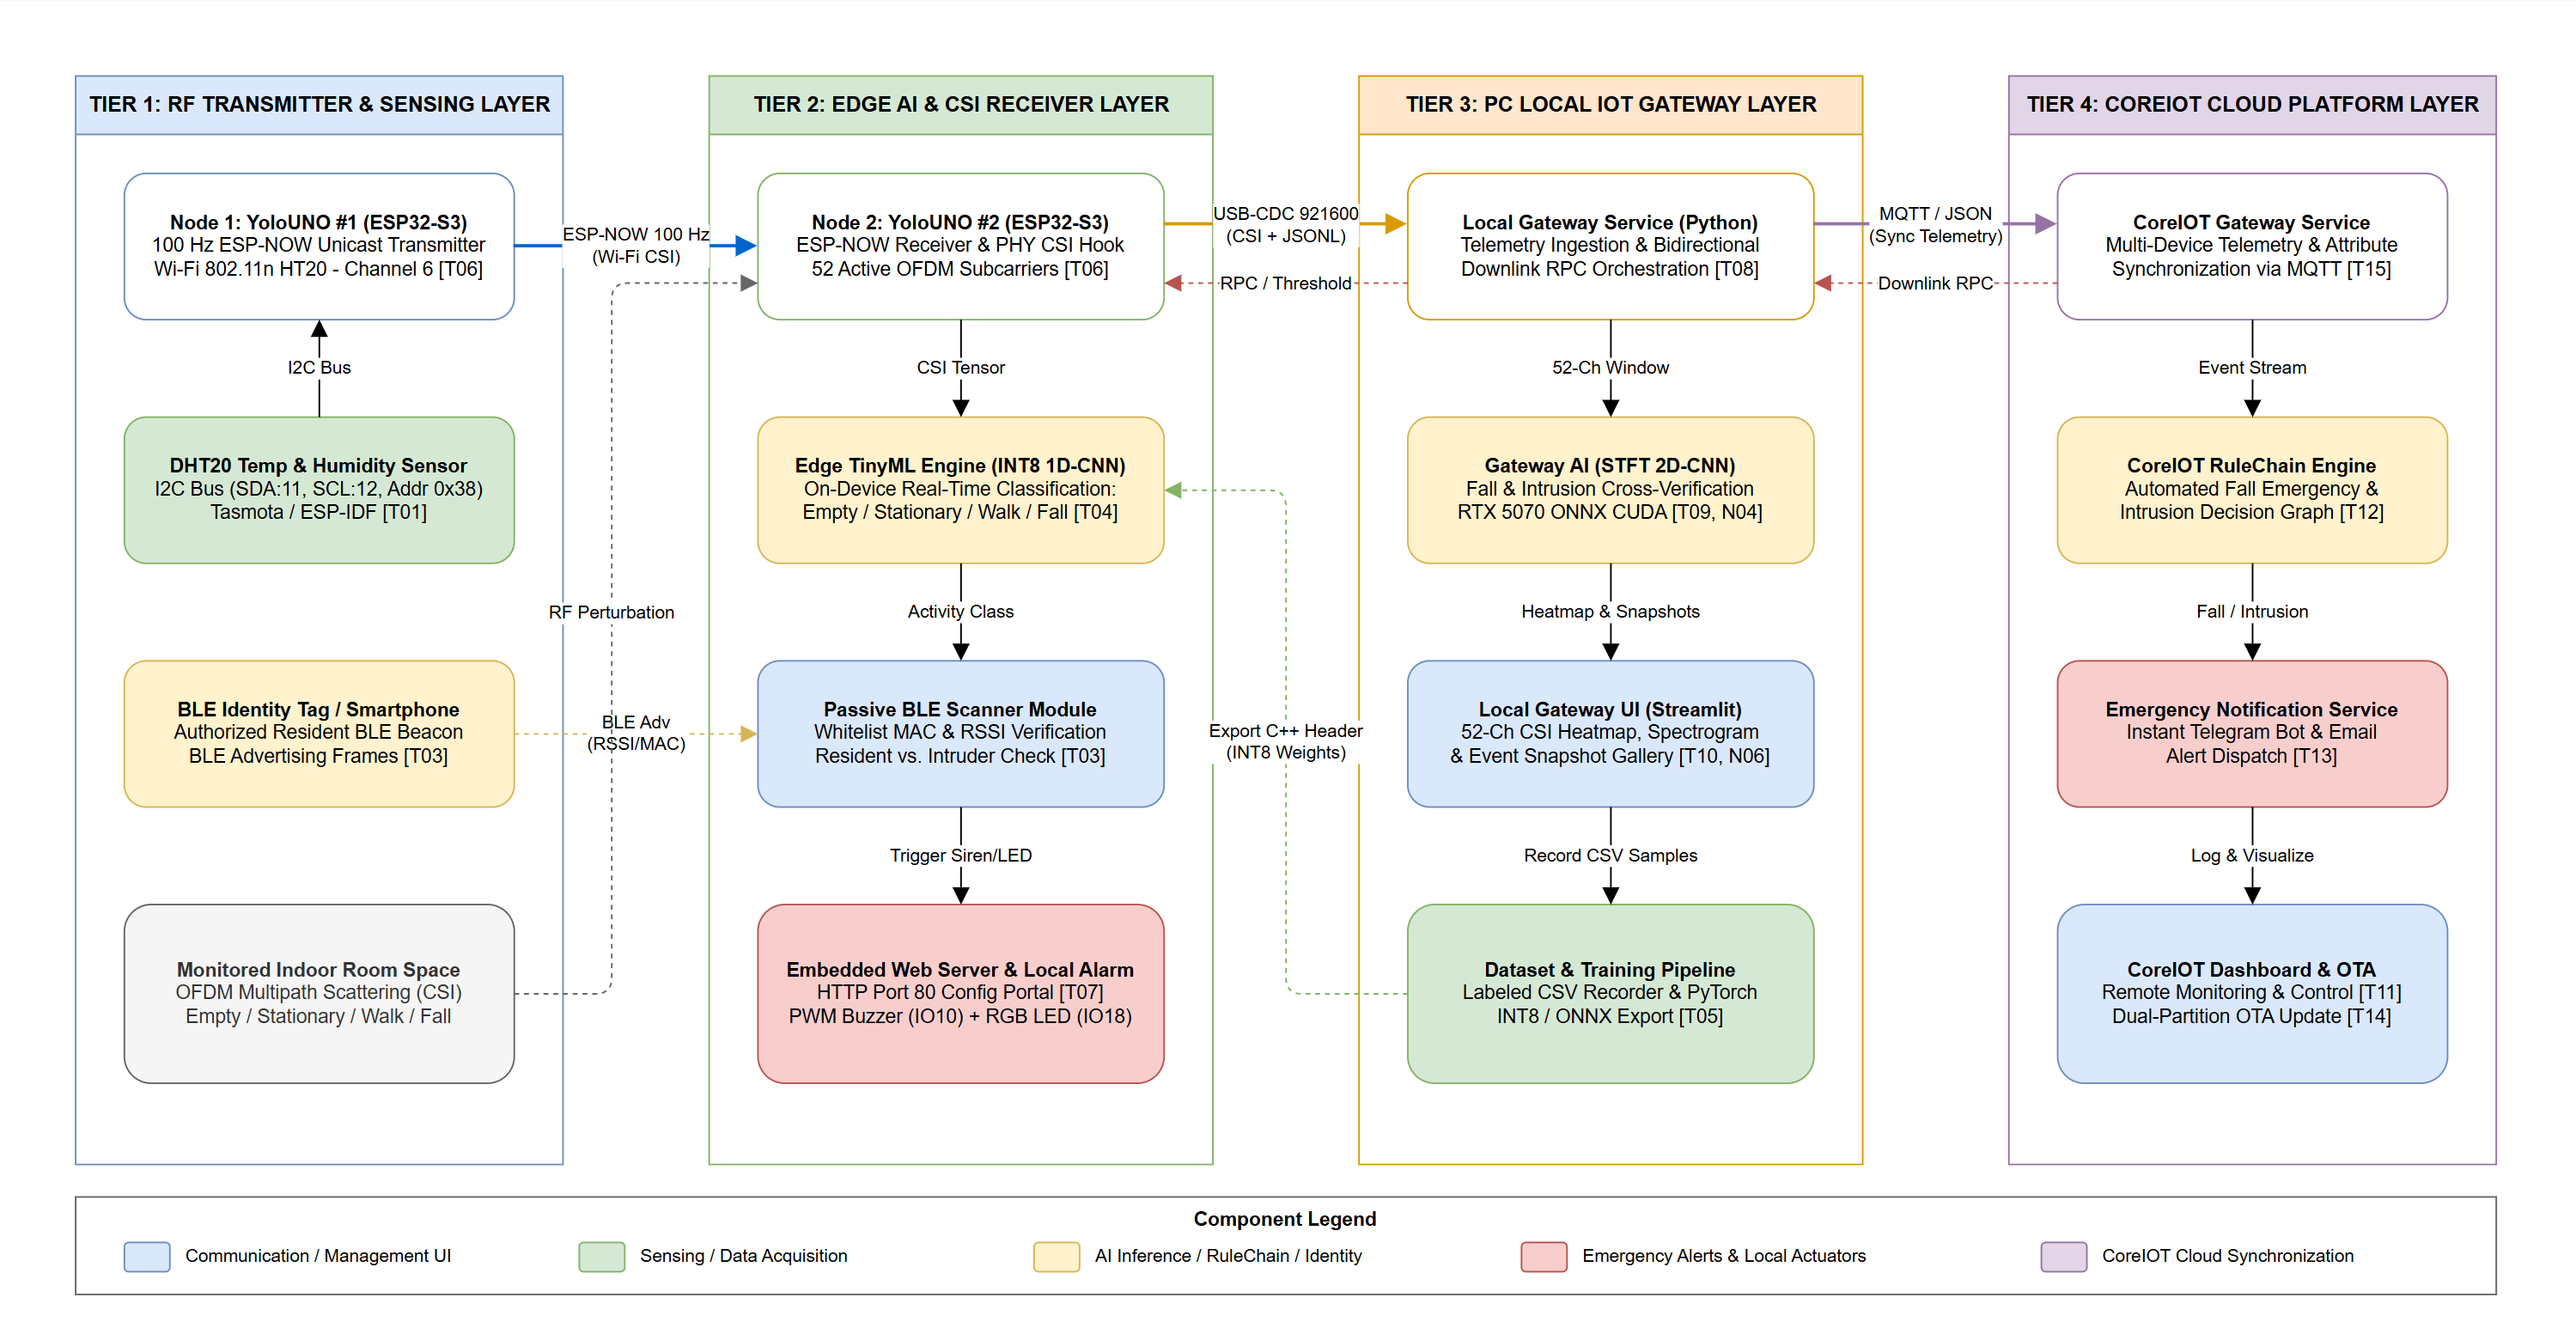
\includegraphics[width=0.98\textwidth]{graphics/en_drawio_overall_architecture.png}
\caption{Four-tier system architecture spanning RF Transmitter \& Sensing (Tier~1), Edge AI \& CSI Receiver (Tier~2), PC Local IoT Gateway with RTX~5070 GPU Acceleration (Tier~3), and CoreIOT Cloud Platform (Tier~4).}
\label{fig:overall_arch}
\end{figure}

The end-to-end dataflow and control loop operate as follows:
\begin{enumerate}
  \item \textbf{Tier~1 (RF Transmitter \& Environmental Sensing):} Node~1 (\texttt{YoloUNO \#1}) locks its Wi-Fi transceiver onto 802.11n 20~MHz Channel~6 ($2437\text{ MHz}$) and transmits deterministic 24-byte unicast ESP-NOW probe packets at exactly $100\text{ Hz}$ (\texttt{T06}). Every $2.0\text{ s}$, Node~1 polls an I2C \textbf{DHT20} sensor (\texttt{T01}) and embeds calibrated ambient temperature and relative humidity directly inside the 24-byte ESP-NOW payload. Simultaneously, authorized residents carry a passive BLE 5.0 beacon tag or smartphone (\texttt{T03}).
  \item \textbf{Tier~2 (Edge AI \& CSI Receiver):} As each 100~Hz ESP-NOW frame traverses the room, human motion perturbs the multipath propagation paths. Node~2 (\texttt{YoloUNO \#2}) extracts the 64-subcarrier complex CSI vector from the Wi-Fi baseband hardware callback, strips null/guard tones to retain 52 active subcarriers, applies causal Hampel despiking and 4th-order Butterworth bandpass filtering, and executes an on-device \textbf{INT8 1D-CNN TinyML} classifier (\texttt{T04}). In parallel on Core~0, Node~2 performs time-sliced passive BLE scanning (\texttt{T03}), hosts an \textbf{Embedded HTTP Web Server} (\texttt{T07}), and drives local PWM buzzer and WS2812B RGB actuators.
  \item \textbf{Tier~3 (PC Local IoT Gateway \& GPU Spectrogram Engine):} Node~2 streams compact JSONL frames over native USB-CDC at $921600\text{ bps}$ into the Python \texttt{LocalIoTGatewayService} (\texttt{T08}). Whenever a $2.0\text{ s}$ window ($200\times 52$) updates, the Gateway computes a 3-band Short-Time Fourier Transform (STFT) spectrogram ($3\times 64\times 64$) and runs a \textbf{2D-CNN} on the \textbf{NVIDIA GeForce RTX~5070 GPU} via ONNX Runtime \texttt{CUDAExecutionProvider} (\texttt{T09}, \texttt{N04}). Confirmed emergencies trigger automatic Hampel-peak highlighting and PNG snapshot recording (\texttt{N06}) on the live \textbf{Streamlit UI} (\texttt{T10}). Crucially, through the Adapter pattern, Tier~3 seamlessly switches between physical Serial (\texttt{COMx}) and \texttt{VirtualYoloUnoCluster} (\texttt{simulator} mode) via a single configuration key.
  \item \textbf{Tier~4 (CoreIOT Cloud Platform):} The PC Gateway multiplexes both nodes over a single persistent MQTT connection (\texttt{v1/gateway/*}, \texttt{T15}) to CoreIOT. A 7-node \textbf{CoreIOT RuleChain} (\texttt{T12}) evaluates fused emergency and intrusion rules, logs cloud alarms onto the remote \textbf{Dashboard} (\texttt{T11}), dispatches instant \textbf{Telegram Bot} alerts (\texttt{T13}), and routes downlink RPC commands and \textbf{Dual-OTA} firmware updates (\texttt{T14}) back to the edge nodes.
\end{enumerate}

\subsection[Functional Decomposition]{Functional Decomposition}
\label{sec:func_decomp}

To maintain modular boundaries across the three team members, the system is decomposed into five orthogonal functional subsystems covering features \texttt{F01}--\texttt{F10}, as depicted in Figure~\ref{fig:func_decomp}. Each subsystem communicates strictly via versioned binary structs (\texttt{csi\_ping\_packet\_t}) or JSON schemas, enabling independent unit testing.

\begin{figure}[H]
\centering
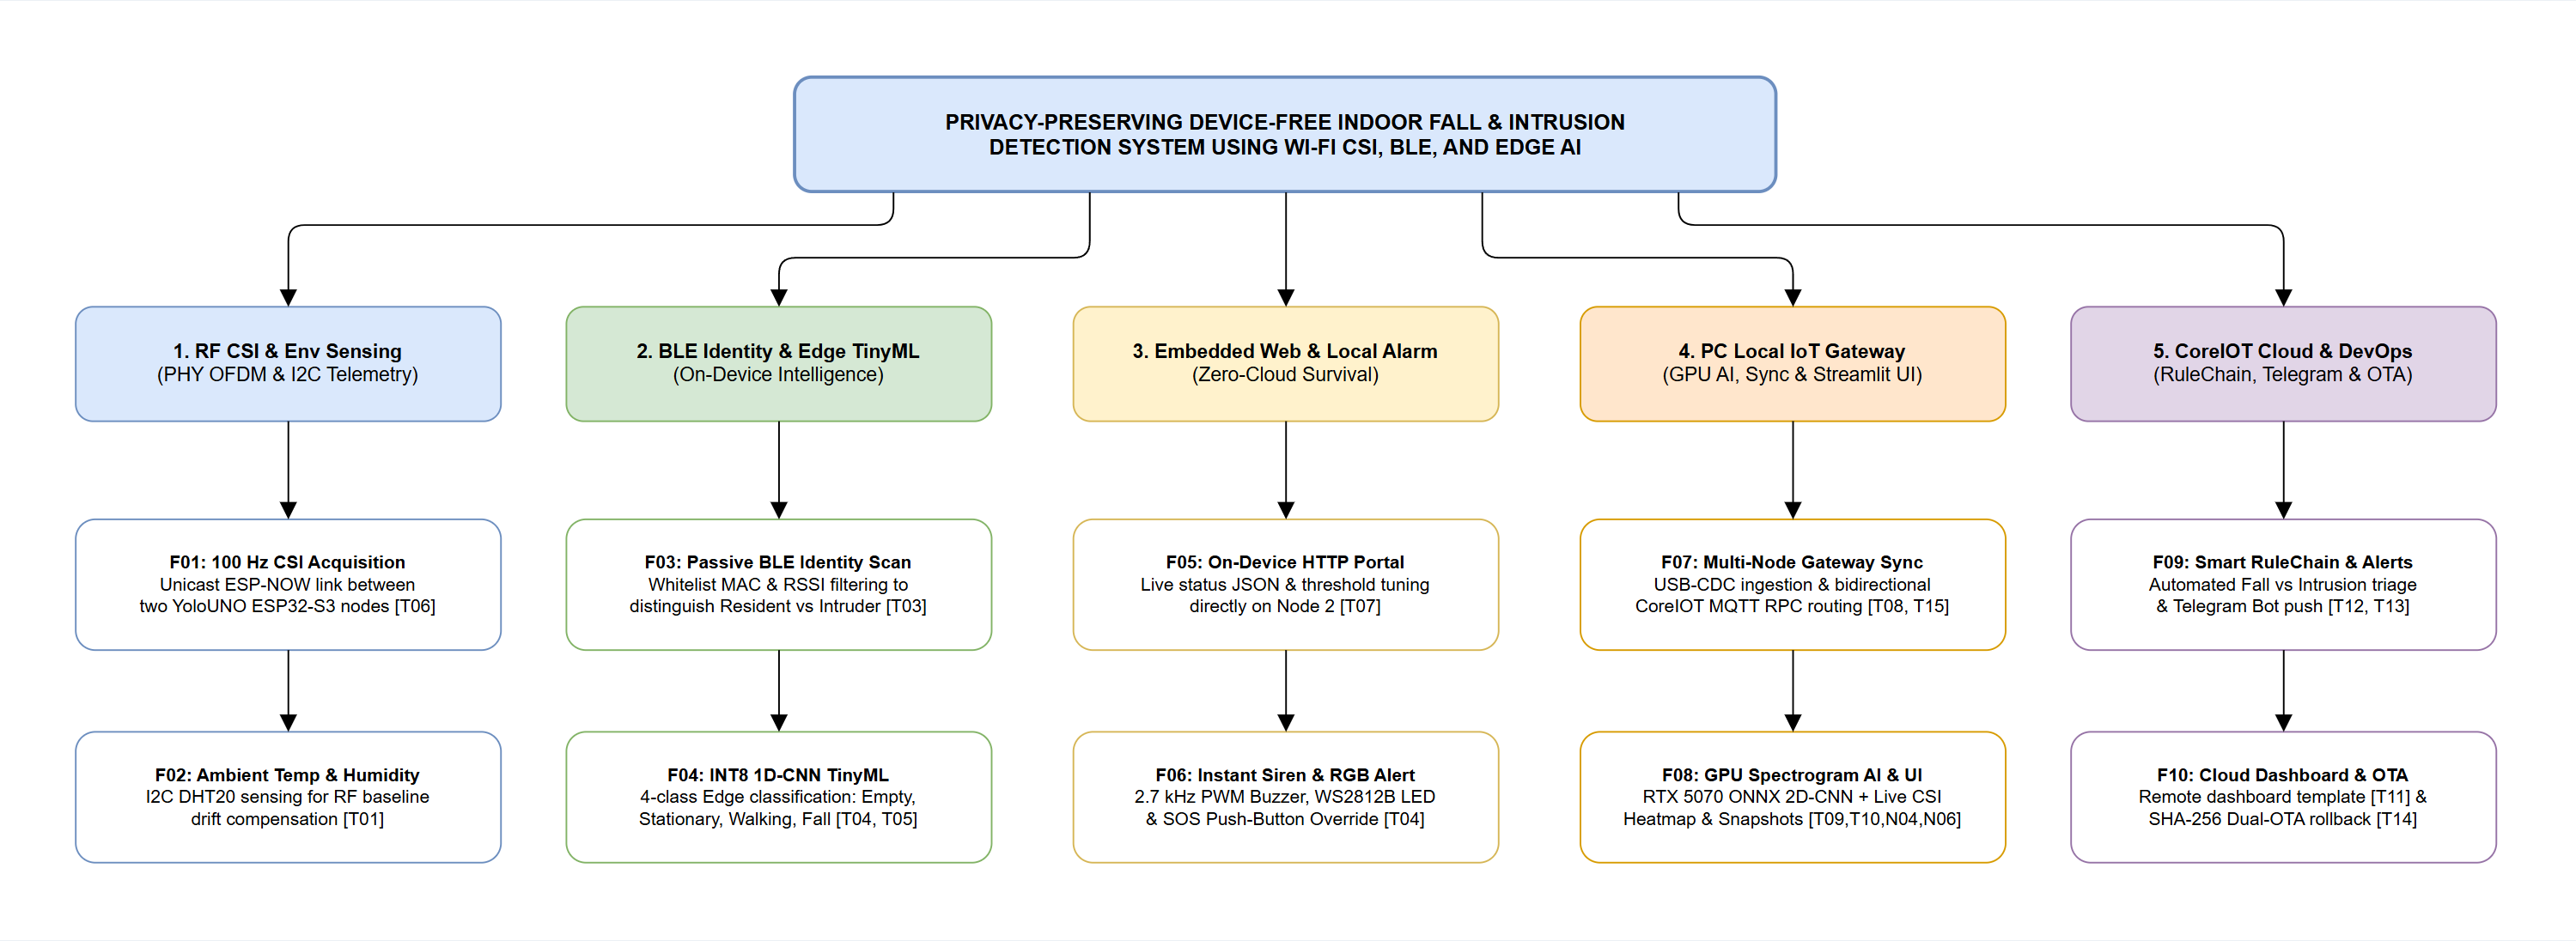
\includegraphics[width=0.98\textwidth]{graphics/en_drawio_functional_decomposition.png}
\caption{Hierarchical functional decomposition of the proposed system into five modular subsystems and ten concrete features (\texttt{F01}--\texttt{F10}).}
\label{fig:func_decomp}
\end{figure}

\subsection[Feature Layer Analysis]{Feature Layer Analysis and Design Rationale}
\label{sec:layer_analysis}

\subsubsection{Sensor Layer (\texttt{T01}, \texttt{T03}, \texttt{T06})}
\label{sec:sensor_layer}

\textbf{Physical Principles of Wi-Fi OFDM Multipath CSI:} In an indoor IEEE 802.11n HT20 channel ($f_c = 2.437\text{ GHz}$, wavelength $\lambda \approx 12.3\text{ cm}$), radio waves propagate from Node~1 to Node~2 along $L$ distinct paths: one static Line-of-Sight (LOS) path, static wall/furniture reflections, and dynamic reflections scattered off a moving human body~\cite{yousefi_survey,zhang_widar}. For each active OFDM subcarrier $k \in \{1,\dots,52\}$ at frequency $f_k = f_c + k\Delta f$ ($\Delta f = 312.5\text{ kHz}$), the complex baseband Channel Frequency Response (CFR) is modeled as:
\begin{equation}
  H_k(t) = I_k(t) + j\,Q_k(t) = H_k^{\text{static}} + \sum_{l \in \Omega_{\text{dyn}}} \alpha_{k,l}(t)\,\exp\!\left(-j\,\frac{2\pi}{\lambda}\,d_l(t)\right) + \eta_k(t)
  \label{eq:csi_multipath}
\end{equation}
where $I_k(t), Q_k(t) \in [-128, 127]$ are signed 8-bit In-phase and Quadrature coefficients captured from the Legacy Long Training Field (LLTF), $d_l(t)$ is the dynamic path length changing at radial velocity $v_r(t) = \frac{dd_l}{dt}$, and $\eta_k(t)$ denotes thermal and Automatic Gain Control (AGC) noise. Because unsynchronized ESP32-S3 oscillators introduce random Carrier Frequency Offset (CFO) and Sampling Frequency Offset (SFO) into raw phase $\angle H_k(t)$, we extract the CFO-invariant subcarrier amplitude $|H_k(t)| = \sqrt{I_k^2(t) + Q_k^2(t)}$. When a human falls, torso acceleration produces a short, high-energy Doppler chirp ($f_D = \frac{2 v_r}{\lambda} \approx 8\text{--}25\text{ Hz}$ lasting $0.35\text{--}0.60\text{ s}$) followed immediately by near-zero floor variance---a time-frequency signature distinctly separable from steady walking ($2\text{--}6\text{ Hz}$ periodic gait) or rapid sitting (decelerated mid-room stop without floor impact).

\textbf{Sensor Selection Trade-Offs:}
\begin{itemize}
  \item \textit{DHT20 I2C vs.\ DHT11 Single-Wire (\texttt{T01}):} We selected the \textbf{Aosong DHT20} over legacy DHT11/DHT22 sensors because DHT20 uses a hardware I2C bus (\texttt{0x38}) with $\pm 0.5^\circ\text{C}$ / $\pm 3\%\text{ RH}$ factory calibration and CRC-8 (\texttt{0x31}) integrity checking. Crucially, bit-banged single-wire sensors disable interrupts for milliseconds and cause jitter in 100~Hz ESP-NOW transmission, whereas hardware I2C leaves Core~1 RF timing untouched while tracking ambient humidity shifts that slowly alter RF dielectric attenuation.
  \item \textit{Passive BLE 5.0 Beacon vs.\ Active Keypad/RFID (\texttt{T03}):} Passive BLE advertising tags require zero user interaction when entering the room, allowing Node~2 to fuse physical motion (\texttt{WALKING}) with proximity authentication ($\text{MAC} \in \mathcal{W}$ and $\text{RSSI} \ge -75\text{ dBm}$).
\end{itemize}

\subsubsection{Communication Layer (\texttt{T06}, \texttt{T08}, \texttt{T15})}
\label{sec:comm_layer}

Table~\ref{tab:comm_choices} summarizes why three distinct communication protocols were selected for the intra-room RF link, edge-to-gateway link, and gateway-to-cloud link.

\begin{table}[H]
\centering
\caption{Design Trade-Offs Across Communication Layer Protocols}
\label{tab:comm_choices}
\footnotesize
\begin{tabularx}{\textwidth}{|P{2.8cm}|P{3.0cm}|P{3.0cm}|Y|}
\hline
\textbf{Link Segment} & \textbf{Chosen Protocol} & \textbf{Rejected Alternative} & \textbf{Engineering Justification} \\
\hline
Node~1 $\rightarrow$ Node~2\newline (100~Hz RF Radar) & Unicast ESP-NOW on fixed Ch.~6 (\texttt{T06}) & UDP/TCP sockets via Wi-Fi Router & Router CSMA/CA contention and beacon DTIM sleep introduce $20\text{--}150\text{ ms}$ jitter that ruins Doppler STFT; raw MAC-layer ESP-NOW achieves $\Delta t = 10.0 \pm 0.4\text{ ms}$ even if the home router loses power. \\
\hline
Node~2 $\leftrightarrow$ PC Gateway\newline (52-Ch Stream) & Native USB-CDC Serial @ 921600~bps (\texttt{T08}) & Wi-Fi TCP / UART 115200~bps & Streaming 52-subcarrier frames over Wi-Fi forces radio TX bursts that blind CSI RX; ESP32-S3 native USB-CDC provides $>70\text{ KB/s}$ deterministic throughput with zero RF self-interference. \\
\hline
PC Gateway $\leftrightarrow$ Cloud\newline (Multi-Node Sync) & CoreIOT Gateway MQTT (\texttt{v1/gateway/*}, \texttt{T15}) & Per-device HTTP REST polling & Single-token MQTT persistent session pushes telemetry and receives downlink RPC in $<80\text{ ms}$ broker RTT instead of high-overhead HTTP polling. \\
\hline
\end{tabularx}
\end{table}

\subsubsection{IoT Gateway Layer (\texttt{T08}, \texttt{T10}, \texttt{N06})}
\label{sec:gateway_layer}

We implemented the PC Local IoT Gateway in Python~3.11 (\texttt{LocalIoTGatewayService}) rather than Node-RED because real-time 52-subcarrier matrix ring buffering, causal Hampel despiking, SciPy STFT spectrogram generation, and GPU ONNX tensor execution require native NumPy/CUDA memory views without JSON serialization bottlenecks between visual flow nodes. For the local operator console (\texttt{T10}), \textbf{Streamlit + Plotly} renders interactive 52-channel CSI heatmaps, $64\times 64$ Doppler spectrograms, RPC control buttons, and automated PNG snapshot galleries (\texttt{N06}) in any standard browser.

\subsubsection{Artificial Intelligence Layer (\texttt{T04}, \texttt{T05}, \texttt{T09}, \texttt{N04})}
\label{sec:ai_layer}

Figure~\ref{fig:ai_pipeline} depicts our 11-step collaborative signal-processing, Edge-GPU AI fusion, and CoreIOT RuleChain pipeline.

\begin{figure}[H]
\centering
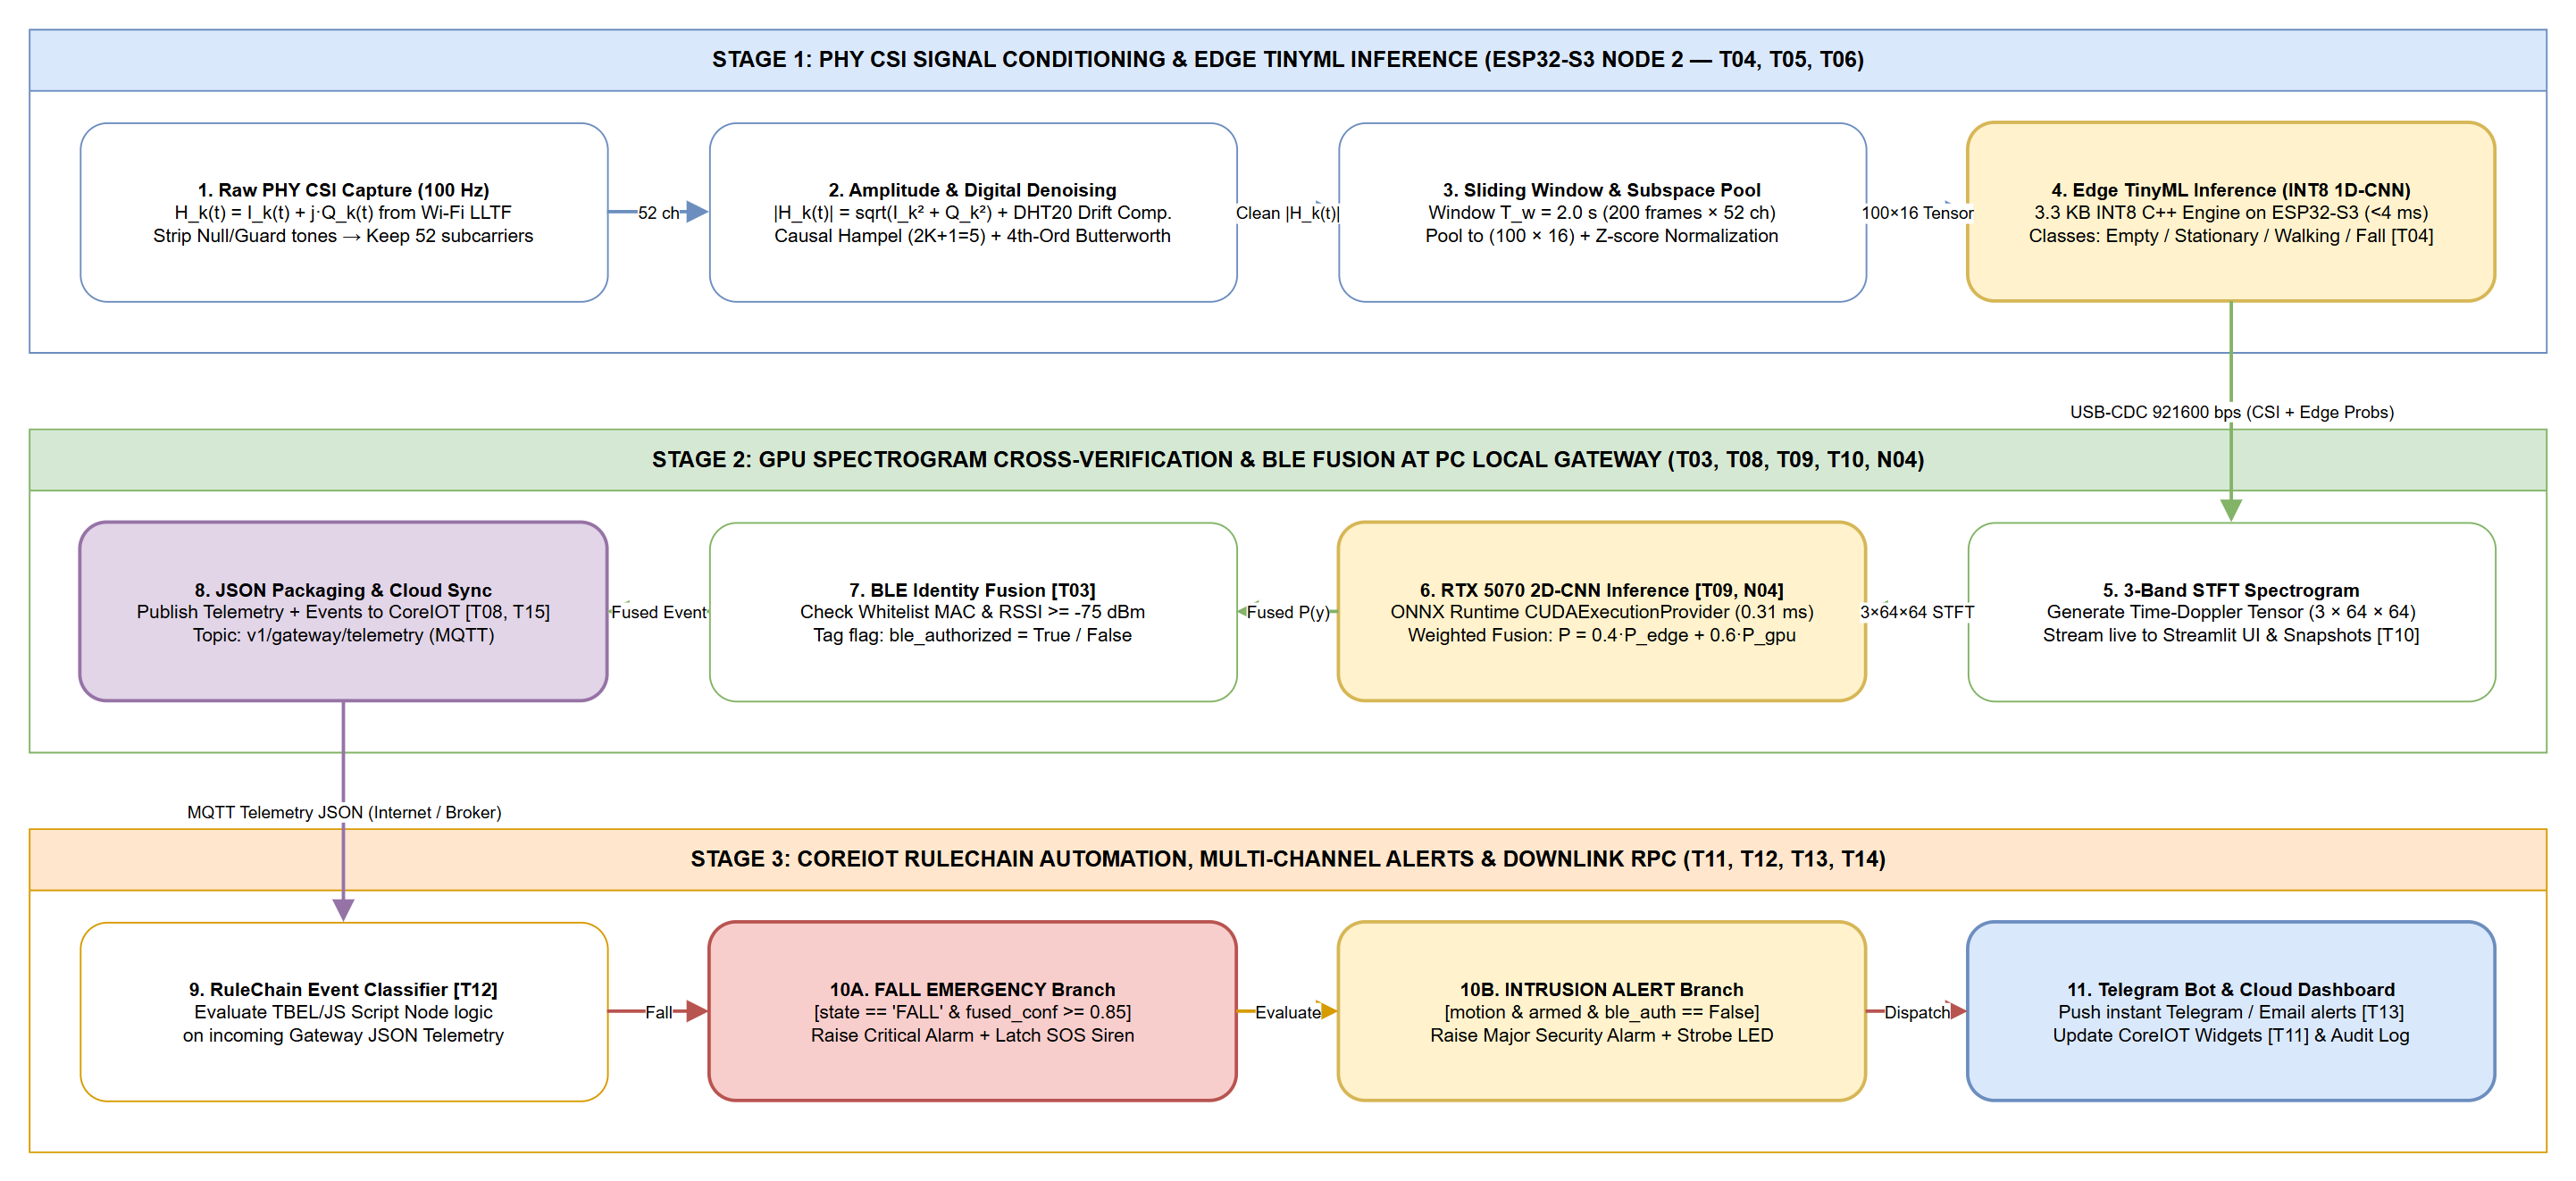
\includegraphics[width=0.98\textwidth]{graphics/en_drawio_ai_rulechain_pipeline.png}
\caption{Three-stage collaborative AI and automation pipeline: (Stage~1) causal CSI conditioning and 3.3~KB INT8 1D-CNN on ESP32-S3; (Stage~2) 3-band STFT Spectrogram 2D-CNN on RTX~5070 ONNX CUDA plus BLE identity fusion; and (Stage~3) CoreIOT RuleChain triage and Telegram alerting.}
\label{fig:ai_pipeline}
\end{figure}

\textbf{Mathematical Formulation of Two-Stage Conditioning \& Fusion:}
\begin{enumerate}
  \item \textbf{Causal Hampel Outlier Rejection:} Wi-Fi receivers occasionally suffer single-frame AGC gain steps. Over a causal 5-point sliding window $W_t = \{|H_k(t-4)|,\dots,|H_k(t)|\}$, we compute the local median $m_k(t) = \text{median}(W_t)$ and scaled Median Absolute Deviation $\hat{\sigma}_k(t) = 1.4826 \cdot \text{median}(|W_t - m_k(t)|)$. Any sample violating $||H_k(t)| - m_k(t)| > 3\,\hat{\sigma}_k(t)$ is replaced by $m_k(t)$ without using future frames.
  \item \textbf{4th-Order Butterworth Bandpass Filter:} Cascaded Second-Order Sections (SOS) isolate human motion frequencies within $[0.25\text{ Hz}, 18.0\text{ Hz}]$ ($f_s = 100\text{ Hz}$), removing static wall multipath DC offsets ($<0.2\text{ Hz}$) and high-frequency switching noise ($>20\text{ Hz}$).
  \item \textbf{Weighted Probability Fusion:} Let $\mathbf{p}_{\text{edge}} \in [0,1]^4$ denote the softmax vector from Node~2's INT8 1D-CNN and $\mathbf{p}_{\text{gpu}} \in [0,1]^4$ denote the softmax vector from the Gateway's STFT 2D-CNN. The fused posterior distribution is computed as:
  \begin{equation}
    \mathbf{p}_{\text{fused}} = \alpha\,\mathbf{p}_{\text{edge}} + (1 - \alpha)\,\mathbf{p}_{\text{gpu}}, \qquad \alpha = 0.40,\; 1-\alpha = 0.60
    \label{eq:prob_fusion}
  \end{equation}
  Assigning weight $0.60$ to the higher-capacity 2D time-frequency spectrogram model suppresses rare single-domain false positives while preserving sensitivity when both models concur. Whenever the Gateway is offline, Node~2 falls back autonomously to $\mathbf{p}_{\text{edge}}$ ($\alpha = 1.0$).
\end{enumerate}

\subsubsection{Application Layer and CoreIOT Platform (\texttt{T11}--\texttt{T15})}
\label{sec:app_layer}

At the cloud application layer, \textbf{CoreIOT} (built on the ThingsBoard IoT architecture) provides unified device-profile management (\texttt{CSI\_Radar\_Profile}), time-series telemetry persistence, low-code TBEL/JavaScript RuleChain execution (\texttt{T12}), Telegram REST webhook integration (\texttt{T13}), interactive remote dashboards (\texttt{T11}), and versioned firmware package hosting for Dual-OTA delivery (\texttt{T14}).

\subsection[Feature - Technology Element Mapping]{Feature -- Technology Element Mapping}
\label{sec:tech_mapping}

Table~\ref{tab:feature_tech_map} provides the complete traceability matrix linking features \texttt{F01}--\texttt{F10} to rubric codes \texttt{T01}--\texttt{T15} and \texttt{N01}/\texttt{N04}/\texttt{N06}.

\begin{table}[H]
\centering
\caption{Traceability Matrix Mapping Features (\texttt{F01}--\texttt{F10}) to Rubric Elements}
\label{tab:feature_tech_map}
\resizebox{\textwidth}{!}{%
\begin{tabular}{|c|l|c|c|c|c|c|c|c|c|c|c|c|c|c|c|c|c|c|}
\hline
\textbf{Feat} & \textbf{Concise Feature Description} & \textbf{T01} & \textbf{T03} & \textbf{T04} & \textbf{T05} & \textbf{T06} & \textbf{T07} & \textbf{T08} & \textbf{T09} & \textbf{T10} & \textbf{T11} & \textbf{T12} & \textbf{T13} & \textbf{T14} & \textbf{T15} & \textbf{N04} & \textbf{N06} & \textbf{N01} \\
\hline
\texttt{F01} & 100~Hz ESP-NOW CSI Link & & & & & \textbf{X} & & & & & & & & & & & & \\
\hline
\texttt{F02} & I2C DHT20 Env Sensing & \textbf{X} & & & & \textbf{X} & & & & & & & & & & & & \\
\hline
\texttt{F03} & Passive BLE Identity Scan & & \textbf{X} & & & & & & & & & & & & & & & \\
\hline
\texttt{F04} & Edge INT8 1D-CNN TinyML & & & \textbf{X} & \textbf{X} & & & & & & & & & & & & & \\
\hline
\texttt{F05} & Node~2 HTTP Web Portal & & & & & & \textbf{X} & & & & & & & & & & & \\
\hline
\texttt{F06} & Siren, RGB \& SOS Button & & & \textbf{X} & & & \textbf{X} & \textbf{X} & & & & & & & & & & \\
\hline
\texttt{F07} & PC Gateway \& Cloud Sync & & & & & & & \textbf{X} & & & & & & & \textbf{X} & & & \\
\hline
\texttt{F08} & GPU 2D-CNN \& Snapshot UI & & & & \textbf{X} & & & & \textbf{X} & \textbf{X} & & & & & & \textbf{X} & \textbf{X} & \textbf{X} \\
\hline
\texttt{F09} & RuleChain \& Telegram Push & & & & & & & & & & & \textbf{X} & \textbf{X} & & \textbf{X} & & & \\
\hline
\texttt{F10} & Cloud Dashboard \& OTA & & & & & & & \textbf{X} & & & \textbf{X} & & & \textbf{X} & \textbf{X} & & & \\
\hline
\end{tabular}%
}
\end{table}

\subsection[New Technologies Beyond Lectures]{New Technologies Beyond Standard Lectures}
\label{sec:new_tech}

Beyond standard classroom topics (basic GPIO, I2C sensors, single-node MQTT telemetry, and basic dashboards), our group researched and implemented three advanced technologies:
\begin{enumerate}
  \item \textbf{Baseband IEEE 802.11n PHY-Layer CSI Extraction on ESP32-S3:} Standard IoT courses use only scalar RSSI, which fluctuates wildly due to constructive/destructive interference. By hooking \texttt{esp\_wifi\_set\_csi\_rx\_cb()} into the ESP32-S3 Wi-Fi MAC/PHY driver with LLTF and HT-LTF enabled~\cite{espressif_csi}, we turn two commodity \$7 microcontrollers into a 52-subcarrier coherent Doppler motion radar.
  \item \textbf{Post-Training Symmetric INT8 Quantization + Blackwell RTX~5070 ONNX CUDA Execution:} On the edge, we wrote a zero-dependency C++17 INT8 inference header (\texttt{tinyml\_infer.h}) verified bit-accurate against Python within $5\times 10^{-4}$ probability tolerance. On the Gateway, we configured PyTorch \texttt{2.11.0+cu128} and ONNX Runtime \texttt{1.23.2} \texttt{CUDAExecutionProvider}~\cite{onnxruntime_docs} to run natively on NVIDIA's latest Blackwell \texttt{sm\_120} architecture (\textbf{RTX~5070 Laptop GPU}).
  \item \textbf{Physics-Grounded Multipath HIL Cluster Simulation:} To enable rigorous software verification prior to hardware arrival, \texttt{csi\_physics\_generator.py} and \texttt{virtual\_node\_simulator.py} synthesize 52-subcarrier frequency-selective fading, path-loss attenuation ($d \in [1.0, 3.5]\text{ m}$), through-wall NLOS attenuation ($-6.5\text{ dB}$ + multipath delay spread), AGC burst spikes, DHT20 thermal drift, BLE RSSI log-distance shadowing, and live HTTP/TCP sockets.
\end{enumerate}

\subsection[Hardware List and Bill of Materials]{Hardware List and Bill of Materials}
\label{sec:bom}

Table~\ref{tab:bom} details the complete hardware Bill of Materials (BOM) required to assemble the physical two-node prototype, totaling approximately \textbf{565,000~VND (\textasciitilde\$22.2~USD)} excluding the existing laptop PC and router.

\begin{table}[htbp]
\centering
\caption{Complete Hardware Bill of Materials (BOM) for the Physical Prototype}
\label{tab:bom}
\footnotesize
\begin{tabularx}{\textwidth}{|C{0.7cm}|P{3.3cm}|P{3.8cm}|C{1.05cm}|R{2.35cm}|Y|}
\hline
\textbf{No.} & \textbf{Component} & \textbf{Key Technical Specifications} & \textbf{Qty} & \textbf{Est.\ Cost} & \textbf{Assigned Role} \\
\hline
1 & YoloUNO Development Board (ESP32-S3) & Dual-core Xtensa LX7 @ 240~MHz, 8~MB Octal PSRAM, 8/16~MB Flash, Wi-Fi 4 + BLE 5.0, USB-C & 2 & 350,000~VND & Node~1 (CSI Tx) \& Node~2 (CSI Rx + TinyML) \\
\hline
2 & Aosong DHT20 Env Sensor Module & I2C addr \texttt{0x38}, 3.3V, $-40$ to $+80^\circ$C ($\pm 0.5^\circ$C), $0$--$100\%$ RH ($\pm 3\%$), Grove 4-pin & 1 & 45,000~VND & Ambient $T$/$RH$ sensing on Node~1 (\texttt{T01}) \\
\hline
3 & BLE 5.0 Beacon Tag (nRF52810 / iBeacon) & 2.4~GHz BLE Adv (200~ms interval), CR2032 coin cell, configurable TxPower & 1 & 85,000~VND & Authorized resident tag (\texttt{T03}; or Smartphone) \\
\hline
4 & KY-012 Piezo Alarm Buzzer Module & 3.3--5V PWM driven ($2.7\text{ kHz}$ resonant peak, $\ge 85\text{ dBA}$ @ 10~cm), S8050 driver & 1 & 15,000~VND & Local fall \& intrusion siren on Node~2 \\
\hline
5 & WS2812B 4-LED RGB Strip + 330~$\Omega$ Res. & Addressable 24-bit GRB, 5V rail, single-wire 800~kHz protocol on GPIO18 & 1 & 20,000~VND & Visual state bar (Green / Amber / Red) \\
\hline
6 & Tactile Push-Button + Breadboard \& Cables & 12$\times$12~mm switch + 100~nF debounce cap + 2$\times$ USB-C data cables + jumpers & 1 set & 50,000~VND & SOS trigger ($>3\text{ s}$) \& alarm mute ($<3\text{ s}$) \\
\hline
7 & Laptop PC (Gateway Host) & Intel/AMD CPU, 16~GB RAM, \textbf{NVIDIA GeForce RTX~5070 Laptop GPU} (CUDA 12.8) & 1 & Existing & Runs Python Gateway, ONNX GPU AI \& Streamlit UI \\
\hline
\multicolumn{4}{|r|}{\textbf{Total Estimated Hardware Procurement Cost}} & \textbf{565,000~VND} & \textbf{\textasciitilde\$22.2~USD (Low-cost residential kit)} \\
\hline
\end{tabularx}
\end{table}

% =========================================================================
% CHAPTER 3. SYSTEM IMPLEMENTATION
% =========================================================================
\section[System Implementation]{System Implementation}
\label{sec:implementation}

\subsection[Hardware and Wiring Diagrams]{Hardware and Wiring Diagrams}
\label{sec:wiring}

Figure~\ref{fig:hw_wiring} presents the complete pin-level hardware schematic for both YoloUNO ESP32-S3 nodes, power rails, pull-up/series protection resistors, and wireless links. Table~\ref{tab:pinout} specifies every physical GPIO connection, and Table~\ref{tab:pio_footprint} reports the verified Flash and SRAM utilization compiled with PlatformIO (\texttt{espressif32 @ 6.9.0}, \texttt{esp32-s3-devkitc-1} target).

\begin{figure}[H]
\centering
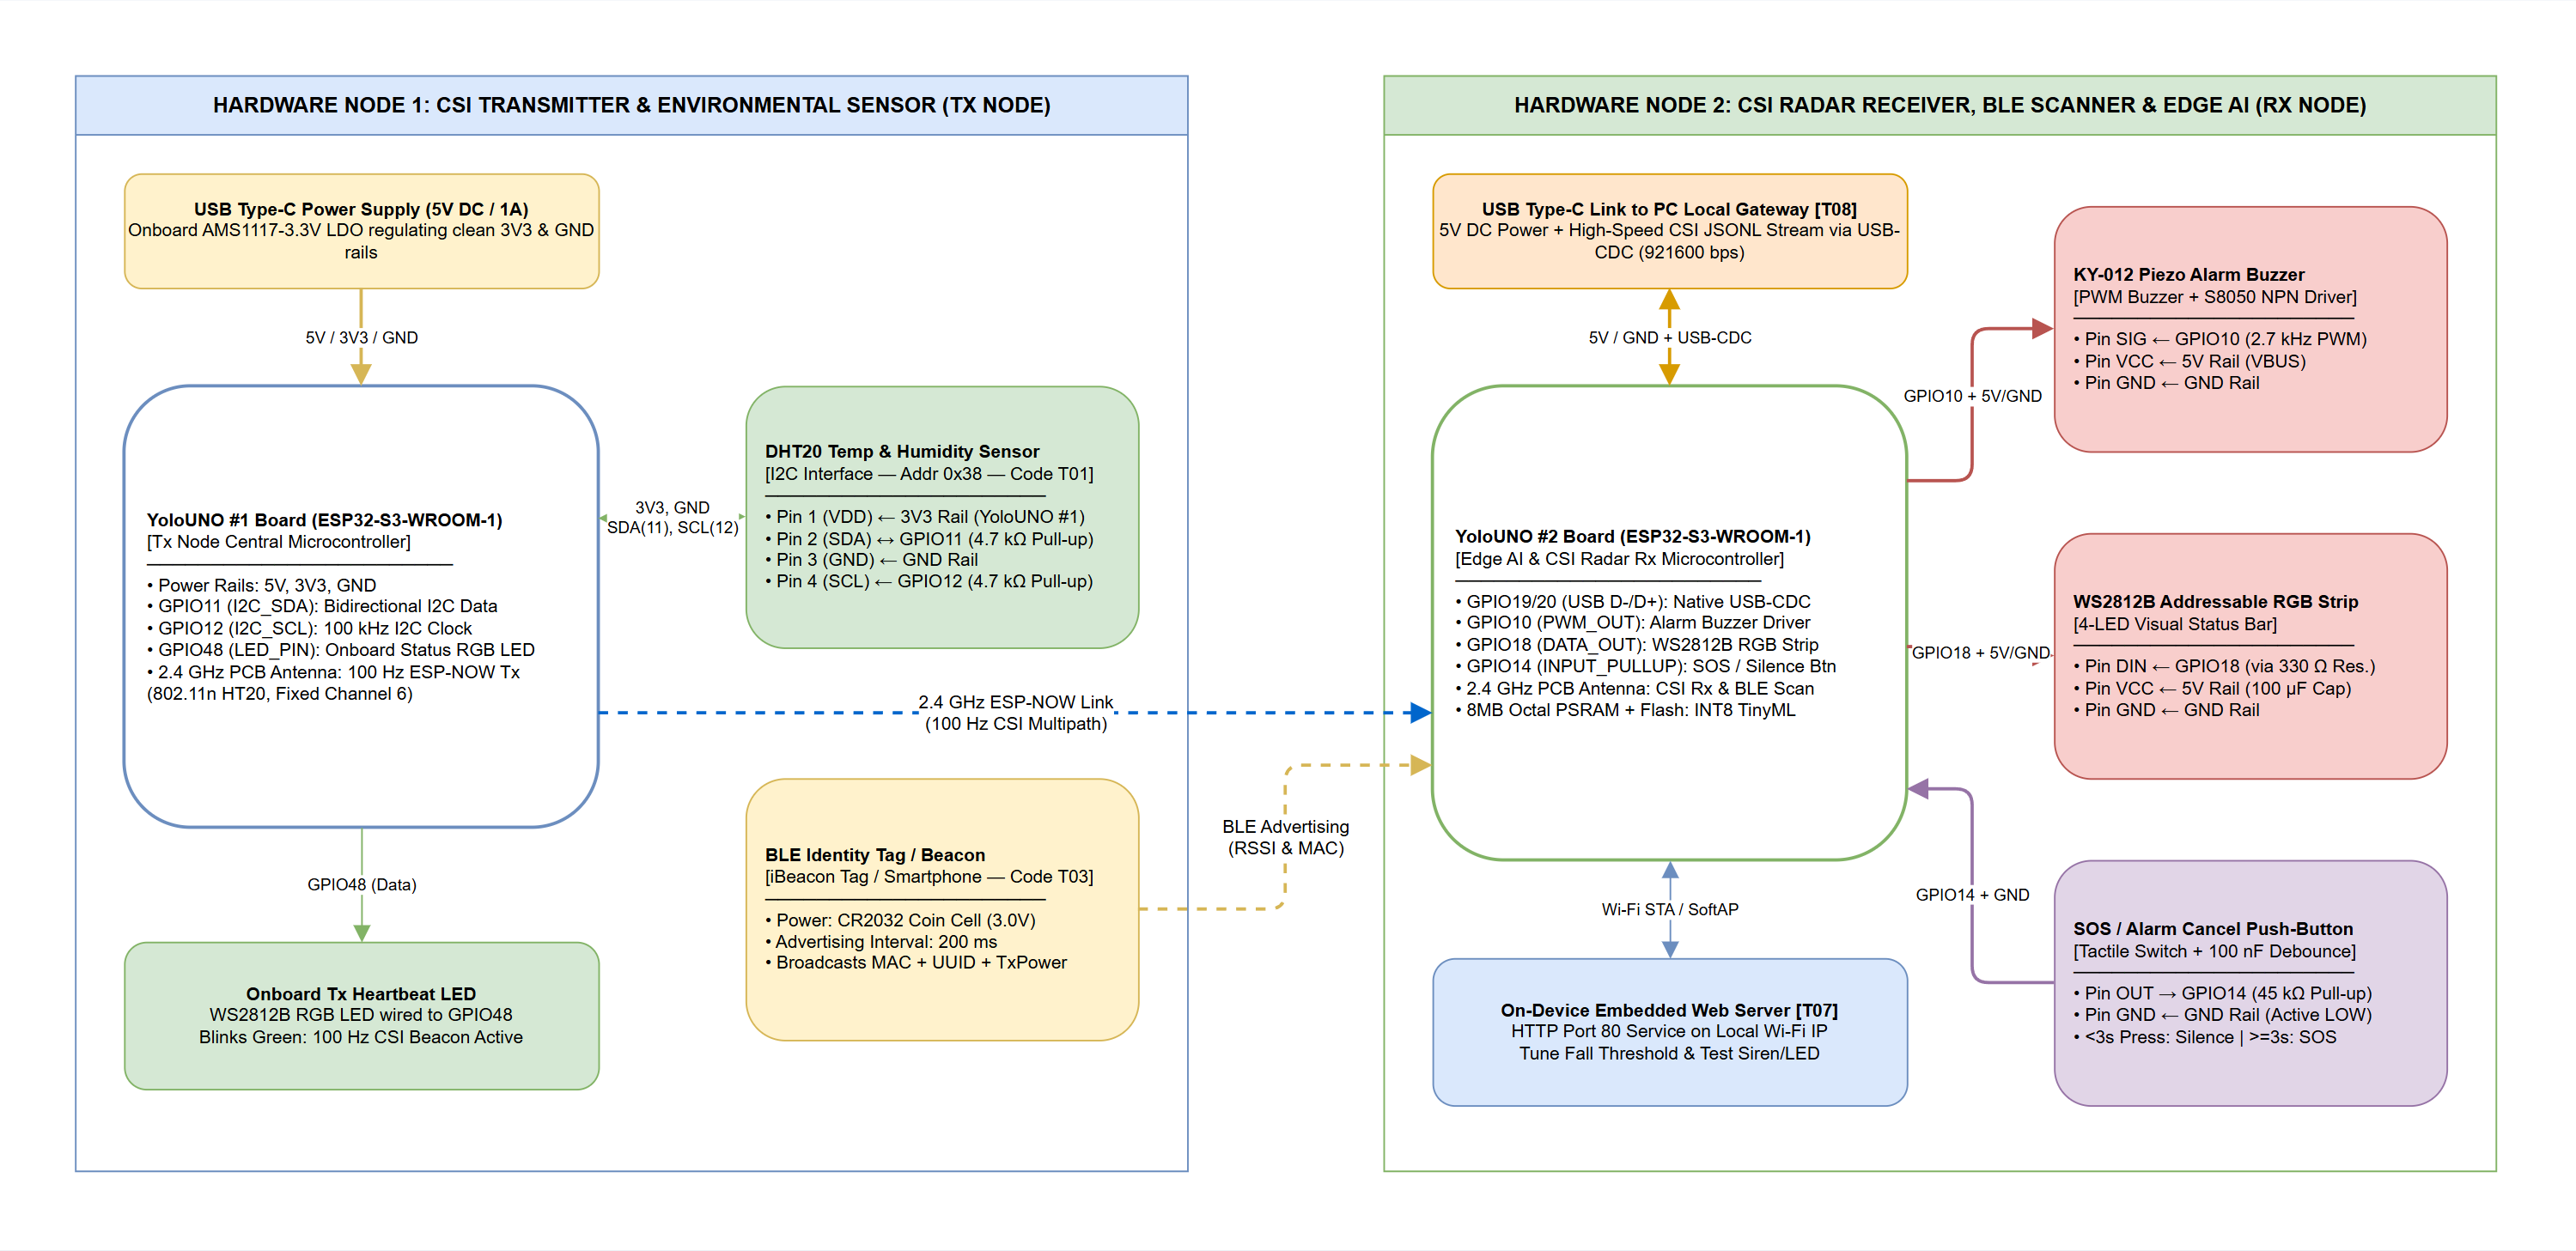
\includegraphics[width=0.98\textwidth]{graphics/en_drawio_hardware_wiring.png}
\caption{Detailed GPIO pinout and wiring schematic for Hardware Node~1 (100~Hz ESP-NOW CSI Transmitter + I2C DHT20) and Hardware Node~2 (CSI Receiver, Passive BLE Scanner, INT8 TinyML, Embedded Web Server, Buzzer, WS2812B RGB, and SOS Button).}
\label{fig:hw_wiring}
\end{figure}

\begin{table}[H]
\centering
\caption{Physical Pin Mapping Table for YoloUNO Node~1 and YoloUNO Node~2}
\label{tab:pinout}
\footnotesize
\begin{tabularx}{\textwidth}{|P{2.2cm}|P{2.7cm}|P{2.4cm}|P{2.2cm}|Y|}
\hline
\textbf{MCU Node} & \textbf{Peripheral} & \textbf{Peripheral Pin} & \textbf{YoloUNO Pin} & \textbf{Electrical Configuration \& Signal Role} \\
\hline
Node~1 (Tx) & DHT20 (\texttt{0x38}) & Pin~1 (\texttt{VDD}) & \texttt{3V3} & Regulated 3.3~V rail from onboard AMS1117-3.3. \\
\hline
Node~1 (Tx) & DHT20 (\texttt{0x38}) & Pin~2 (\texttt{SDA}) & \texttt{GPIO11} & Hardware I2C0 Data, $4.7\text{ k}\Omega$ pull-up to \texttt{3V3}. \\
\hline
Node~1 (Tx) & DHT20 (\texttt{0x38}) & Pin~3 (\texttt{GND}) & \texttt{GND} & Common signal ground. \\
\hline
Node~1 (Tx) & DHT20 (\texttt{0x38}) & Pin~4 (\texttt{SCL}) & \texttt{GPIO12} & Hardware I2C0 Clock ($100\text{ kHz}$ standard mode). \\
\hline
Node~1 (Tx) & Onboard RGB & \texttt{DIN} & \texttt{GPIO48} & Blinks green every 100 transmitted CSI frames. \\
\hline
Node~2 (Rx) & Native USB-CDC & \texttt{D-} / \texttt{D+} & \texttt{GPIO19/20} & 921600~bps JSONL telemetry + downlink RPC link to PC. \\
\hline
Node~2 (Rx) & KY-012 Buzzer & \texttt{SIG} / \texttt{VCC} & \texttt{GPIO10} / \texttt{5V} & LEDC Timer~0 PWM @ $2.7\text{ kHz}$ ($50\%$ duty on alarm). \\
\hline
Node~2 (Rx) & WS2812B 4-LED & \texttt{DIN} / \texttt{VCC} & \texttt{GPIO18} / \texttt{5V} & $330\text{ }\Omega$ series data resistor + $100\text{ }\mu\text{F}$ rail decoupling. \\
\hline
Node~2 (Rx) & SOS Push-Button & \texttt{OUT} / \texttt{GND} & \texttt{GPIO14} / \texttt{GND} & Active-LOW (\texttt{INPUT\_PULLUP}); $<3\text{ s}$ mutes, $\ge 3\text{ s}$ raises SOS. \\
\hline
\end{tabularx}
\end{table}

\begin{table}[H]
\centering
\caption{Verified PlatformIO Binary Compilation Footprint (\texttt{pio run -e yolo\_uno})}
\label{tab:pio_footprint}
\small
\begin{tabularx}{\textwidth}{|P{3.6cm}|R{2.4cm}|R{2.7cm}|R{2.5cm}|Y|}
\hline
\textbf{Firmware Target} & \textbf{Binary Size} & \textbf{Flash Usage (\texttt{ota\_0})} & \textbf{SRAM Usage} & \textbf{Key Linked Modules} \\
\hline
\texttt{node1\_tx\_env} & 895,344~B & 28.5\% (894,981 / 3,145,728~B) & 14.2\% (46,380 / 327,680~B) & WiFi, ESP-NOW, Wire (DHT20), HTTPClient, Update (SHA-256 OTA) \\
\hline
\texttt{node2\_rx\_edge\_ai} & 1,491,120~B & 47.4\% (1,490,749 / 3,145,728~B) & 35.3\% (115,576 / 327,680~B) & WiFi CSI ISR, NimBLE/BLE, INT8 1D-CNN, WebServer, Update \\
\hline
\end{tabularx}
\end{table}

\subsection[Device Firmware]{Device Firmware Implementation}
\label{sec:firmware}

\subsubsection[Node 1 Firmware (\texttt{node1\_tx\_env})]{Node 1 -- ESP-NOW Transmitter \& I2C DHT20 (\texttt{T01}, \texttt{T06}, \texttt{T14})}
\label{sec:fw_node1}

Node~1 (\texttt{firmware/\allowbreak node1\_tx\_env/\allowbreak src/\allowbreak main.cpp}) runs two pinned FreeRTOS tasks: \texttt{Task\_Env\_DHT20} on Core~0 (polling I2C address \texttt{0x38} every $2000\text{ ms}$ with polynomial \texttt{0x31} CRC-8 verification) and \texttt{Task\_CSI\_Beacon} on Core~1 (invoking \texttt{vTaskDelayUntil} every $10\text{ ms}$ to transmit 24-byte \texttt{csi\_ping\_packet\_t} frames on locked Channel~6). Listing~\ref{lst:node1_code} shows the core 100~Hz transmitter loop and Tasmota \texttt{Rule1} equivalent documented in \texttt{tasmota\_yolo\_uno\_dht20.md}.

\begin{lstlisting}[language=C++,caption={Deterministic 100 Hz ESP-NOW CSI Beacon Task on Node 1 (firmware/node1\_tx\_env/src/main.cpp)},label={lst:node1_code}]
void Task_CSI_Beacon(void* pvParameters) {
  TickType_t xLastWake = xTaskGetTickCount();
  const TickType_t xPeriod = pdMS_TO_TICKS(10); // Exact 100 Hz period
  uint32_t seq = 0;
  for (;;) {
    vTaskDelayUntil(&xLastWake, xPeriod);
    csi_ping_packet_t pkt{};
    pkt.magic      = CSI_MAGIC_HEADER; // 0xA55A
    pkt.version    = CSI_PROTO_VER;    // 0x01
    pkt.node_id    = 1;
    pkt.seq_num    = seq++;
    pkt.tx_ms      = millis();
    pkt.temp_c_x100 = g_temp_c_x100;   // From DHT20 (I2C 0x38, CRC-8 0x31)
    pkt.humi_x100   = g_humi_x100;
    pkt.flags       = g_dht_valid ? 0x01 : 0x00;
    pkt.crc8        = compute_crc8_0x07(reinterpret_cast<const uint8_t*>(&pkt), sizeof(pkt) - 1);
    esp_now_send(PEER_RX_MAC, reinterpret_cast<const uint8_t*>(&pkt), sizeof(pkt));
  }
}
// Tasmota ESP32-S3 Template & Rule1 (T01 validation):
// Template: {"NAME":"YoloUNO-S3-DHT20","GPIO":[0,0,0,0,0,0,0,640,608,0,0,0,0,0],"FLAG":0,"BASE":1}
// Rule1 ON Tele-AHT2X#Temperature DO Publish stat/yolo_node1/ENV {"temp":%value%} ENDON
\end{lstlisting}

\subsubsection[Node 2 Firmware (\texttt{node2\_rx\_edge\_ai})]{Node 2 -- CSI Radar, Passive BLE \& TinyML (\texttt{T03}, \texttt{T04}, \texttt{T06}, \texttt{T14})}
\label{sec:fw_node2}

Because Node~2 simultaneously handles 100~Hz Wi-Fi baseband interrupts, passive BLE scanning, digital filtering, neural network inference, HTTP serving, and OTA updates, naïve single-core execution would starve the CSI callback or trigger Watchdog resets. As shown in Figure~\ref{fig:fw_ota_arch}, we strictly partition tasks across the two Xtensa LX7 cores of the ESP32-S3:
\begin{itemize}
  \item \textbf{Core~1 (Real-Time Signal \& AI Engine):} Executes the \texttt{IRAM\_ATTR} \texttt{wifi\_csi\_rx\_cb()} callback, pushes raw 52-subcarrier amplitudes into a 64-slot lock-free FreeRTOS queue (\texttt{xQueueCSI}), runs causal Hampel + 4th-order Butterworth SOS filtering (\texttt{csi\_dsp.h}), executes the INT8 1D-CNN every $200\text{ ms}$ ($20$-frame stride over a $200$-frame sliding window), drives local GPIO10/GPIO18 alarms, and streams JSONL over USB-CDC.
  \item \textbf{Core~0 (Wireless Protocol \& Service Stack):} Handles \texttt{onEspNowDataRecv()}, runs \texttt{Task\_BLE\_Scanner} (\texttt{ble\_scanner.h}), serves Port~80 HTTP endpoints (\texttt{web\_server.h}), polls the GPIO14 SOS button, and executes \texttt{CoreIOTOtaUpdater} (\texttt{ota\_updater.h}). Inter-core state sharing is protected by a lightweight spinlock (\texttt{portMUX\_TYPE g\_stateMux}).
\end{itemize}

\begin{figure}[H]
\centering
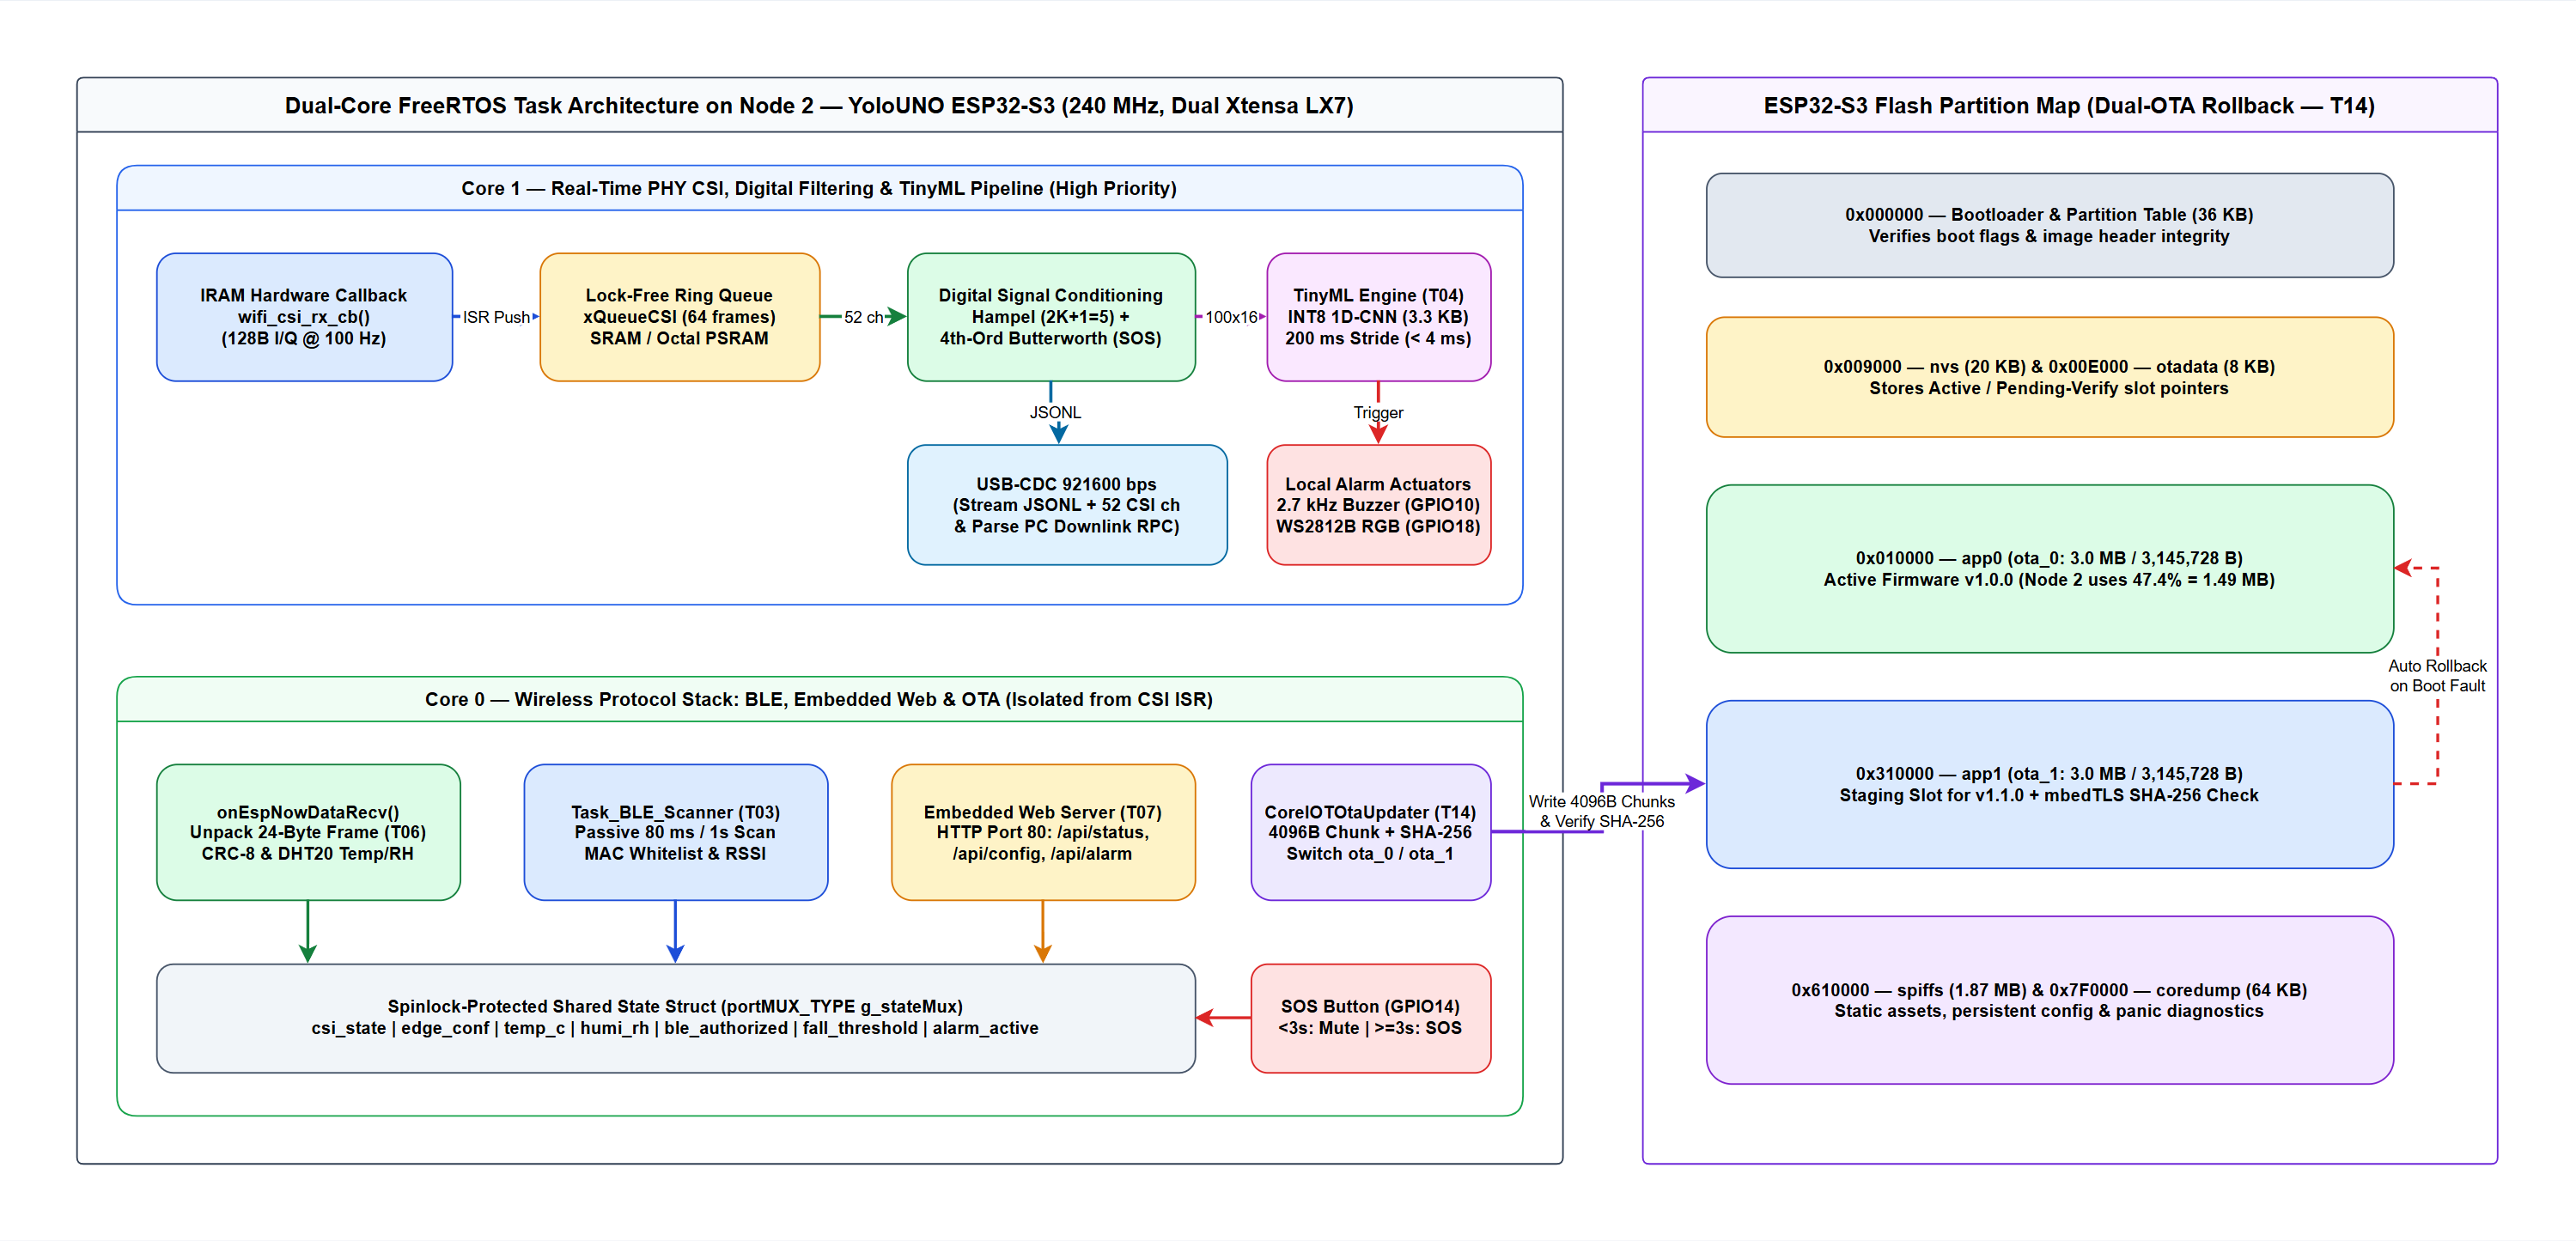
\includegraphics[width=0.98\textwidth]{graphics/en_drawio_firmware_ota_architecture.png}
\caption{Dual-core FreeRTOS task isolation on Node~2 (Core~1 real-time CSI/DSP/TinyML vs.\ Core~0 BLE/HTTP/OTA) and symmetric \texttt{ota\_0}/\texttt{ota\_1} Flash partition layout.}
\label{fig:fw_ota_arch}
\end{figure}

\subsubsection[On-Device Web Server (\texttt{T07})]{On-Device Embedded Web Server (\texttt{T07})}
\label{sec:web_server}

Implemented in \texttt{firmware/\allowbreak node2\_rx\_edge\_ai/\allowbreak include/\allowbreak web\_server.h}, Node~2 hosts a lightweight dark-mode HTML5/AJAX control portal on HTTP Port~80 with zero external CDN dependencies (so it works on isolated LANs without Internet). It exposes four REST endpoints: \texttt{GET /} (dashboard UI), \texttt{GET /api/status} (live TinyML class, confidence, DHT20 temperature/humidity, packet loss, and BLE MAC/RSSI), \texttt{POST /api/config} (on-the-fly adjustment of \texttt{fall\_threshold}, \texttt{ble\_rssi\_min}, and \texttt{security\_armed}), and \texttt{POST /api/alarm} (manual siren test/mute). Figure~\ref{fig:node2_web} shows the live rendered portal during an active fall emergency.

\begin{figure}[H]
\centering
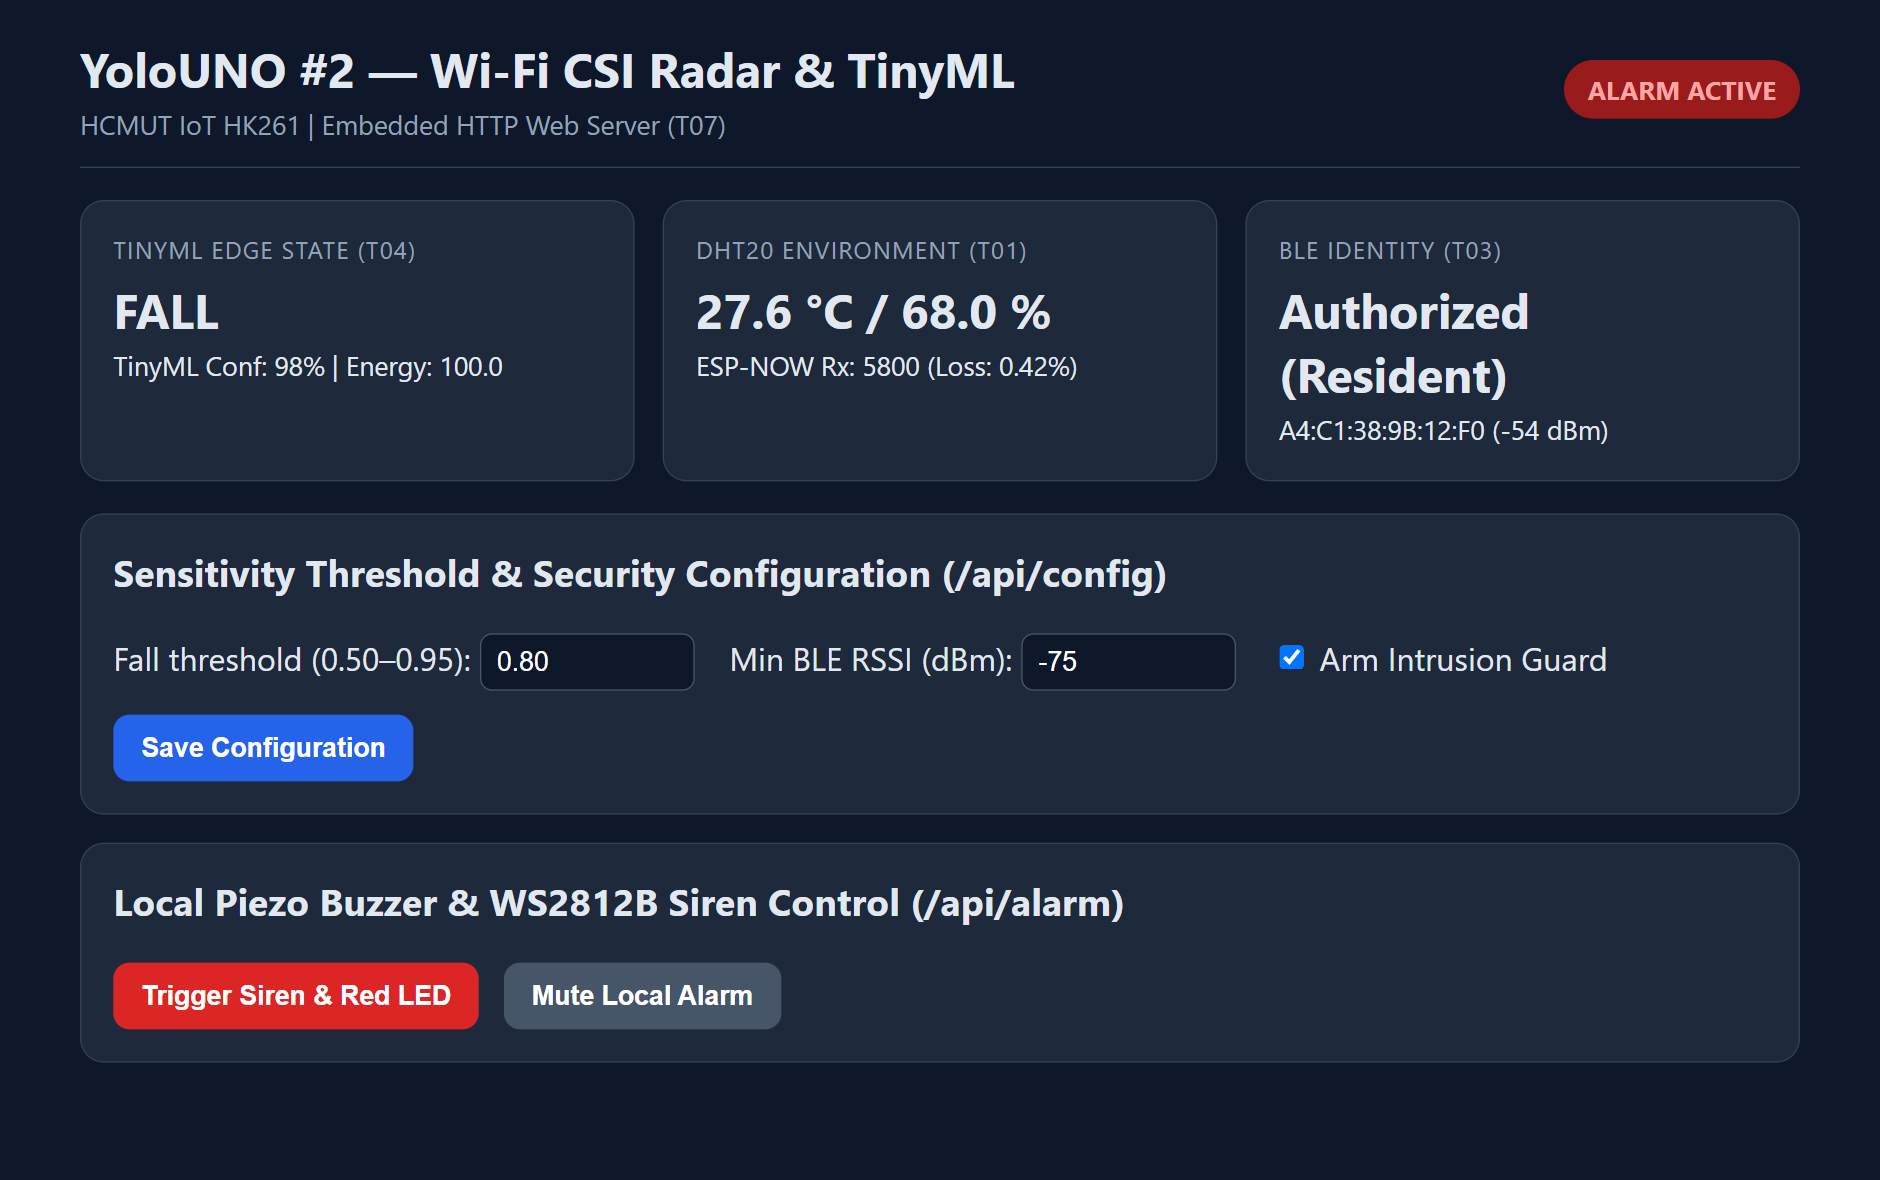
\includegraphics[width=0.88\textwidth]{graphics/ui_node2_embedded_web.png}
\caption{Live screenshot of Node~2's Embedded HTTP Web Server (\texttt{T07}) displaying real-time \texttt{FALL} detection (\texttt{TinyML Conf: 98\%}), DHT20 telemetry (\texttt{27.6~$^\circ$C / 68.0~\%}), authorized resident BLE tag (\texttt{A4:C1:38:9B:12:F0, -54~dBm}), threshold configuration, and manual siren controls.}
\label{fig:node2_web}
\end{figure}

\subsection[Device-to-Device Communication]{Device-to-Device Communication (\texttt{T03}, \texttt{T06})}
\label{sec:d2d_comm}

Table~\ref{tab:packet_layout} defines the exact 24-byte packed binary frame (\texttt{csi\_ping\_packet\_t} in \texttt{firmware/\allowbreak include/\allowbreak csi\_protocol.h}) sent at $100\text{ Hz}$ from Node~1 to Node~2. Using \texttt{\#pragma pack(push, 1)} guarantees byte-level layout compatibility across Xtensa compilers, while CRC-8 (\texttt{0x07}) rejects corrupted air frames before updating environmental registers.

\begin{table}[H]
\centering
\caption{Binary Frame Layout of the 24-Byte \texttt{csi\_ping\_packet\_t} ESP-NOW Payload}
\label{tab:packet_layout}
\footnotesize
\begin{tabularx}{\textwidth}{|C{1.5cm}|P{2.8cm}|P{2.2cm}|C{1.3cm}|Y|}
\hline
\textbf{Offset} & \textbf{Field Name} & \textbf{C++ Type} & \textbf{Size} & \textbf{Description \& Encoding} \\
\hline
\texttt{0..1} & \texttt{magic} & \texttt{uint16\_t} & 2~B & Frame sync word fixed to \texttt{0xA55A} (little-endian). \\
\hline
\texttt{2} & \texttt{version} & \texttt{uint8\_t} & 1~B & Protocol version (\texttt{0x01}). \\
\hline
\texttt{3} & \texttt{node\_id} & \texttt{uint8\_t} & 1~B & Transmitter node identifier (\texttt{0x01} = YoloUNO \#1). \\
\hline
\texttt{4..7} & \texttt{seq\_num} & \texttt{uint32\_t} & 4~B & Monotonic counter used by Node~2 to compute packet-loss rate. \\
\hline
\texttt{8..11} & \texttt{tx\_ms} & \texttt{uint32\_t} & 4~B & Node~1 uptime timestamp in milliseconds. \\
\hline
\texttt{12..13} & \texttt{temp\_c\_x100} & \texttt{int16\_t} & 2~B & Ambient temperature $\times 100$ (e.g., \texttt{2745} $= 27.45^\circ$C). \\
\hline
\texttt{14..15} & \texttt{humi\_x100} & \texttt{uint16\_t} & 2~B & Relative humidity $\times 100$ (e.g., \texttt{6820} $= 68.20\%$ RH). \\
\hline
\texttt{16} & \texttt{flags} & \texttt{uint8\_t} & 1~B & Bit~0: \texttt{dht20\_valid}; Bit~1: \texttt{ota\_pending}. \\
\hline
\texttt{17..22} & \texttt{reserved} & \texttt{uint8\_t[6]} & 6~B & Zero-padded alignment reserved for multi-zone expansion. \\
\hline
\texttt{23} & \texttt{crc8} & \texttt{uint8\_t} & 1~B & CRC-8/ITU (\texttt{poly=0x07}) computed over bytes \texttt{0..22}. \\
\hline
\end{tabularx}
\end{table}

\textbf{Wi-Fi CSI and BLE 5.0 Time-Sliced Coexistence:} On ESP32-S3, Wi-Fi and BLE share a single 2.4~GHz RF front-end via hardware arbiter. Continuous active BLE scanning steals the antenna for $>50\%$ of each second and causes severe CSI frame drops. We solved this in \texttt{ble\_scanner.h} by configuring \textbf{passive} BLE scanning (\texttt{setActiveScan(false)}) with a short $80\text{ ms}$ scan window once every $1000\text{ ms}$ ($8\%$ RF duty cycle) and a $6.0\text{ s}$ authorization TTL cache, preserving $>99\%$ ESP-NOW CSI continuity. Listing~\ref{lst:jsonl_frame} shows an actual USB-CDC JSONL telemetry line emitted by Node~2 to the PC Gateway.

\begin{lstlisting}[caption={Sample JSONL Telemetry Frame Streamed from Node 2 over USB-CDC (921600 bps)},label={lst:jsonl_frame}]
{"seq":4640,"temp_c":27.60,"humi_rh":68.30,"pkt_loss_pct":0.42,"ble_authorized":true,"ble_mac":"A4:C1:38:9B:12:F0","ble_rssi":-55,"edge_state":"FALL","edge_conf":0.981,"edge_probs":[0.001,0.004,0.014,0.981],"amps_52":[24.3,25.1,26.8,"...",21.9]}
\end{lstlisting}

\subsection[PC Local IoT Gateway]{PC Local IoT Gateway (\texttt{T08}, \texttt{T09}, \texttt{T10}, \texttt{T15})}
\label{sec:gateway_impl}

Implemented in \texttt{gateway/\allowbreak main\_gateway.py} (\texttt{LocalIoTGatewayService}) and \texttt{gateway/\allowbreak streamlit\_ui.py}, the PC Local IoT Gateway bridges the high-rate USB-CDC edge link with GPU spectrogram inference and CoreIOT Cloud:
\begin{itemize}
  \item \textbf{Dual-Source Telemetry Ingestion (\texttt{T08}):} When \texttt{source\_mode: "serial"}, a background reader parses $921600\text{ bps}$ JSONL frames from \texttt{COMx} into a 200-frame ring buffer. When \texttt{source\_mode: "simulator"}, it attaches seamlessly to \texttt{VirtualYoloUnoCluster}, executing the exact same DSP, INT8 TinyML, ONNX CUDA 2D-CNN, and MQTT sync code paths.
  \item \textbf{Bidirectional Downlink RPC Router (\texttt{T08}, \texttt{T15}):} Incoming RPC methods from CoreIOT (\texttt{setAlarm}, \texttt{setSecurityArmed}, \texttt{setFallThreshold}, \texttt{triggerOtaUpdate}) or local Streamlit controls are translated into compact newline-terminated ASCII commands (\texttt{RPC:ALARM:1}, \texttt{RPC:ARM:1}, \texttt{RPC:THRESHOLD:0.85}, \texttt{RPC:OTA:1.1.0:<sha256>}) written back down USB-CDC to Node~2.
  \item \textbf{Interactive Streamlit Monitoring \& Control UI (\texttt{T10}):} Shown in Figure~\ref{fig:streamlit_ui}, the local console provides four specialized tabs: (1) Live 52-Subcarrier CSI Heatmap \& $64\times 64$ STFT Spectrogram with Tier-1 vs.\ Tier-2 probability bars; (2) Automatic Event Snapshot Gallery (\texttt{N06}); (3) CoreIOT MQTT \& RuleChain Inspector (\texttt{T12}, \texttt{T15}); and (4) Natural-Language Telemetry Assistant (\texttt{N01}).
\end{itemize}

\begin{figure}[htbp]
\centering
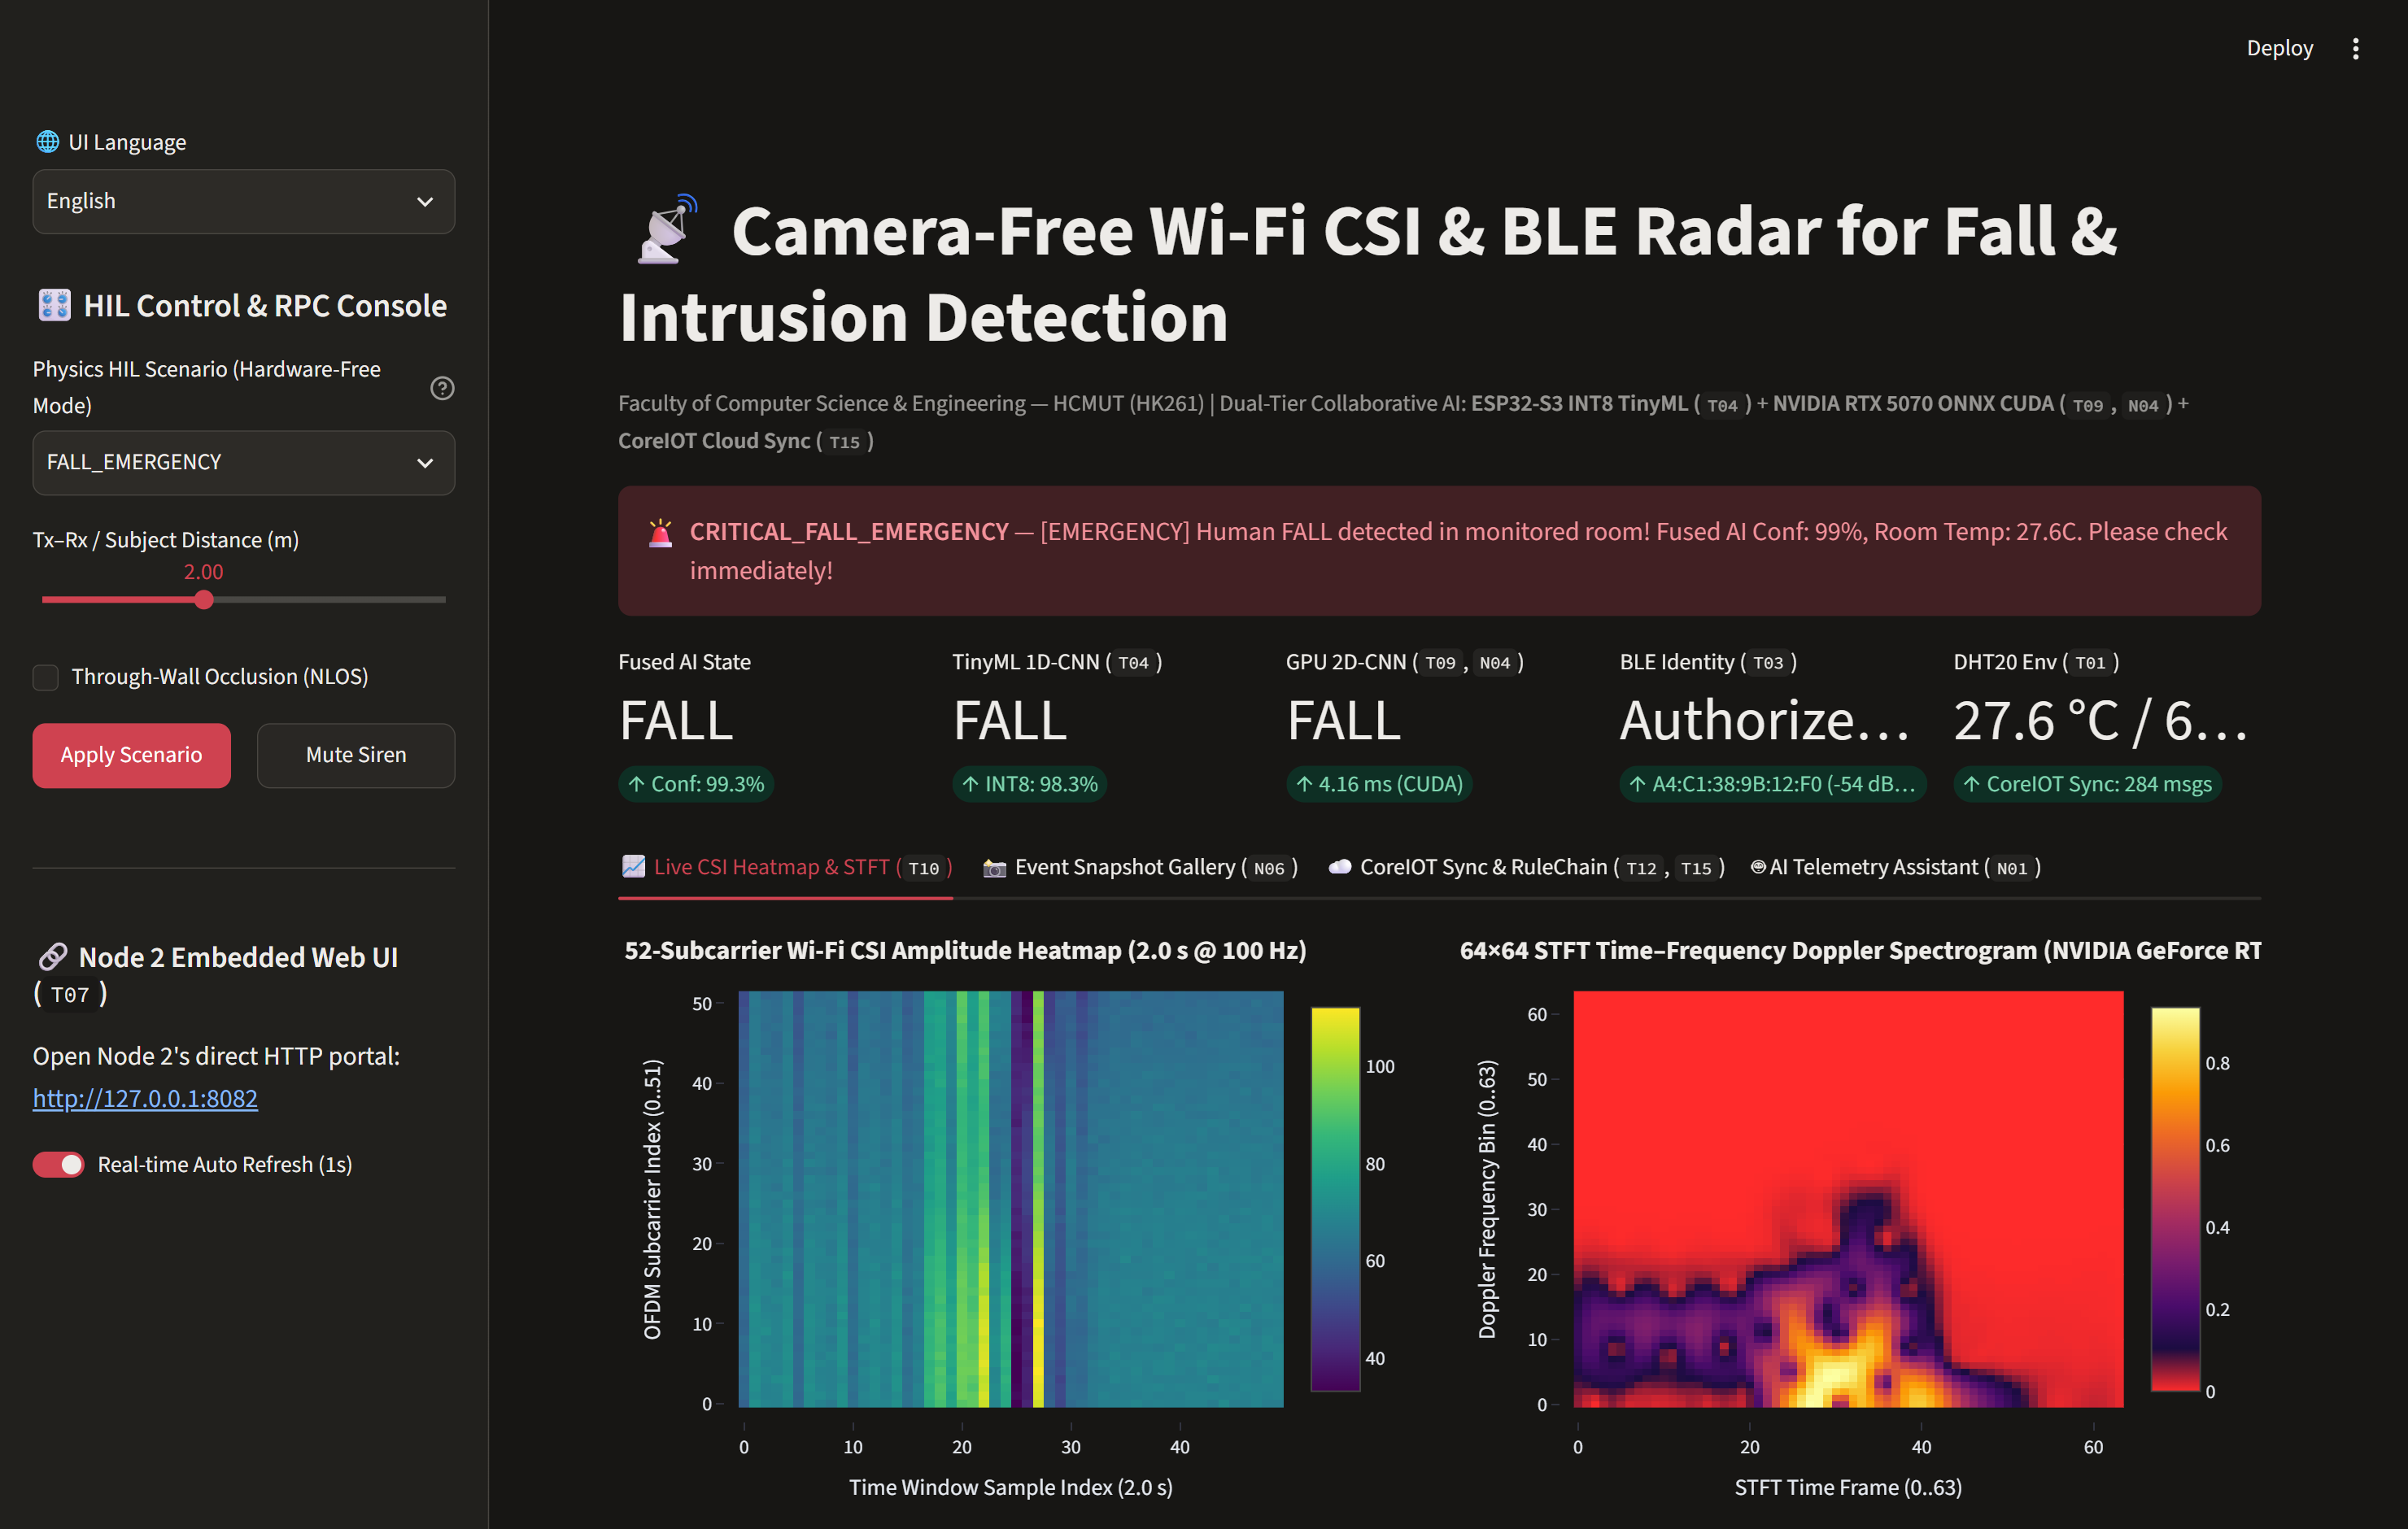
\includegraphics[width=0.98\textwidth]{graphics/ui_gateway_streamlit_dashboard.png}
\caption{Live screenshot of the PC Local IoT Gateway Streamlit Dashboard (\texttt{T10}, \texttt{N04}, \texttt{N06}) running on the NVIDIA GeForce RTX~5070 Laptop GPU (\texttt{4.16~ms CUDA} full-window pipeline), showing real-time \texttt{CRITICAL\_FALL\_EMERGENCY} banner, 52-subcarrier CSI heatmap, and $64\times 64$ STFT Doppler spectrogram.}
\label{fig:streamlit_ui}
\end{figure}

\subsection[Artificial Intelligence Pipeline]{Artificial Intelligence Pipeline (\texttt{T04}, \texttt{T05}, \texttt{T09}, \texttt{N04})}
\label{sec:ai_impl}

\subsubsection[Dataset Generation \& Spectrograms]{Data Collection and Preparation (\texttt{T05})}
\label{sec:dataset}

We built two complementary data tools in \texttt{ai\_training/}: (1) \texttt{csi\_serial\_collector.py} (plus an integrated recorder inside \texttt{streamlit\_ui.py}) for capturing labeled $2.0\text{ s}$ CSV windows from live COM ports, and (2) \texttt{csi\_physics\_generator.py}, which synthesizes physically grounded 52-subcarrier CSI streams across diverse room distances ($1.0\text{--}3.5\text{ m}$), LOS/NLOS wall losses, walking speeds, rapid-sitting hard negatives, random AGC spikes, and thermal drift. Our generated dataset (\texttt{dataset/\allowbreak csi\_multimodal\_dataset.npz} plus \texttt{empty.csv}, \texttt{stationary.csv}, \texttt{walking.csv}, \texttt{fall.csv}) comprises \textbf{1,400 windows} ($350$ per class $\times 4$ classes $= 280,000$ CSI frames $\times 52$ subcarriers), partitioned via stratified split into \textbf{78\% Train (1,092 windows)} and \textbf{22\% Held-Out Test (308 windows)}.

Figure~\ref{fig:spectrograms} illustrates representative STFT Doppler spectrograms across the four classes: \texttt{EMPTY} exhibits broadband low-amplitude thermal noise; \texttt{STATIONARY} concentrates energy near $0\text{--}2\text{ Hz}$ (chest respiration micro-motion); \texttt{WALKING} exhibits sustained periodic $6\text{--}22\text{ Hz}$ torso/limb harmonics across the entire $2.0\text{ s}$ window; and \texttt{FALL} displays an unmistakable impulsive Doppler burst around $t \approx 0.6\text{--}1.0\text{ s}$ followed by complete post-impact silence.

\begin{figure}[H]
\centering
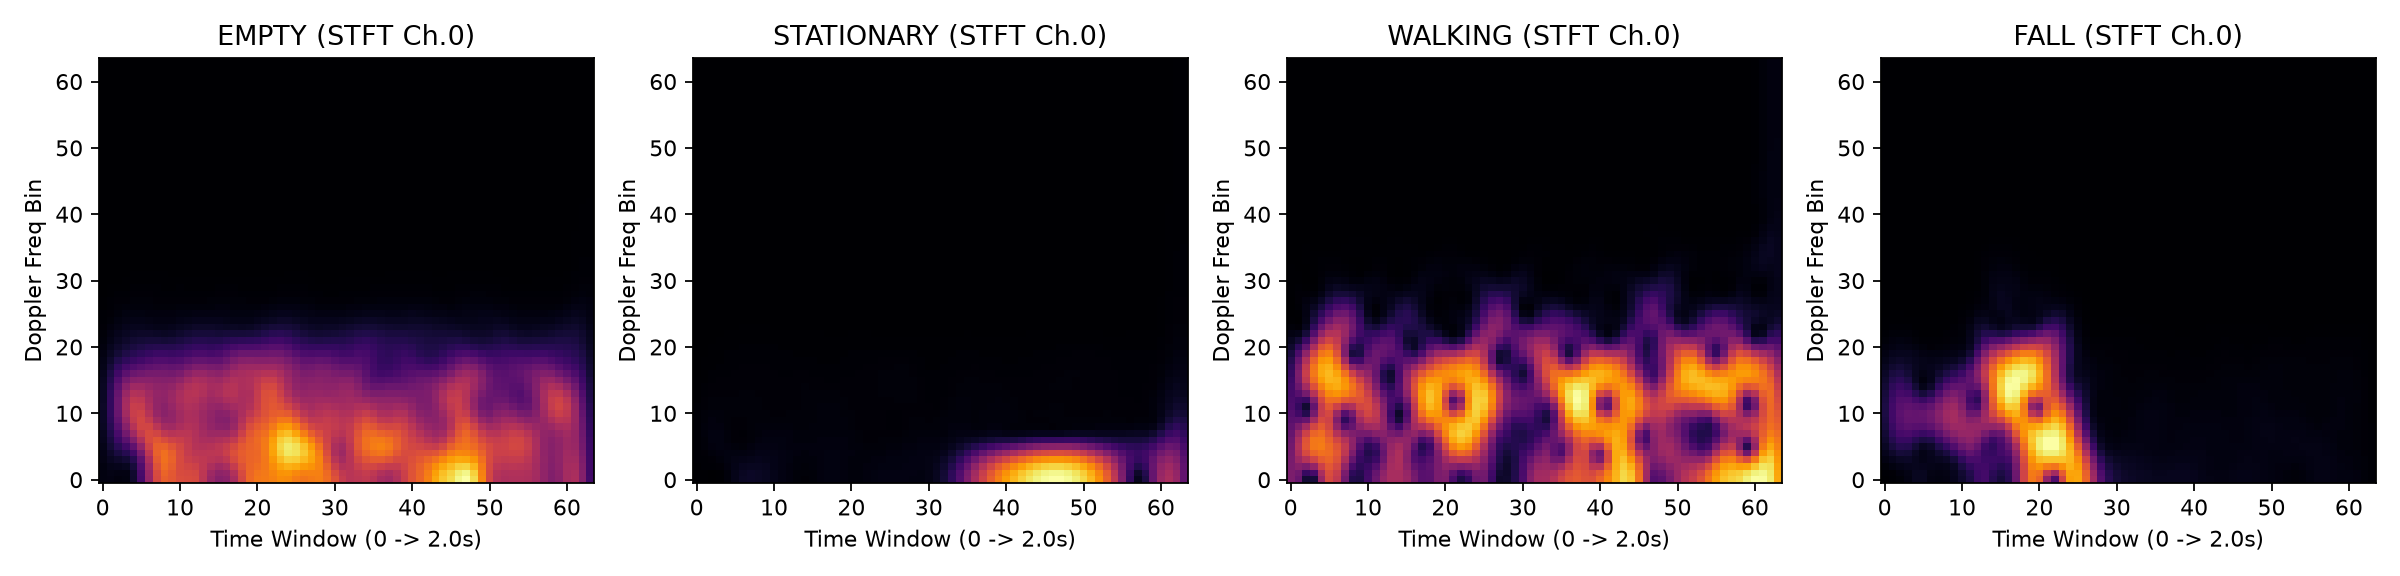
\includegraphics[width=0.98\textwidth]{graphics/csi_class_spectrograms.png}
\caption{Comparison of $64\times 64$ STFT Doppler spectrograms across the four activity classes (\texttt{EMPTY}, \texttt{STATIONARY}, \texttt{WALKING}, and \texttt{FALL}), illustrating the sharp impact-then-silence signature of human falls.}
\label{fig:spectrograms}
\end{figure}

\subsubsection[Model Training and Evaluation]{Model Architectures, Training, and Evaluation (\texttt{T04}, \texttt{T09})}
\label{sec:training}

Both neural networks were trained in PyTorch \texttt{2.11.0+cu128} on our local \textbf{NVIDIA GeForce RTX~5070 Laptop GPU} (reproducible scripts \texttt{train\_tinyml\_1dcnn.py}, \texttt{train\_gpu\_2dcnn.py}, and notebooks \texttt{train\_1dcnn\_tinyml.ipynb}, \texttt{train\_2dcnn\_gpu.ipynb}):
\begin{itemize}
  \item \textbf{Tier~1 Edge TinyML 1D-CNN (\texttt{T04}):} Input tensor $(100\times 16)$ formed by $2\times$ temporal pooling and 16-band subcarrier grouping $\rightarrow$ \texttt{Conv1D(16->24, k=5, ReLU)} + \texttt{MaxPool1D(2)} $\rightarrow$ \texttt{Conv1D(24->32, k=3, ReLU)} + \texttt{GlobalAvgPool1D} $\rightarrow$ \texttt{Linear(32->4)}. Trained for 65 epochs in \textbf{4.30~s} on RTX~5070, achieving \textbf{97.08\% FP32 accuracy} and \textbf{96.75\% INT8 accuracy} (Fall F1 $= \mathbf{94.87\%}$), as shown in Figure~\ref{fig:tinyml_cm}.
  \item \textbf{Tier~2 Gateway STFT Spectrogram 2D-CNN (\texttt{T09}, \texttt{N04}):} Input tensor $(3\times 64\times 64)$ computed from three OFDM subcarrier groups (low, mid, high sub-bands) $\rightarrow$ three \texttt{Conv2D + BatchNorm + ReLU + MaxPool2D} blocks ($16 \rightarrow 32 \rightarrow 64$ filters) $\rightarrow$ \texttt{AdaptiveAvgPool2D(2,2)} $\rightarrow$ \texttt{Linear(256->64->4)}. Trained for 45 epochs in \textbf{4.81~s} on RTX~5070, achieving \textbf{99.68\% test accuracy}, \textbf{99.68\% Macro F1}, and \textbf{100.0\% Fall F1} ($77/77$ test falls detected with zero false alarms), as shown in Figure~\ref{fig:gpu_eval} (left).
\end{itemize}

\begin{figure}[H]
\centering
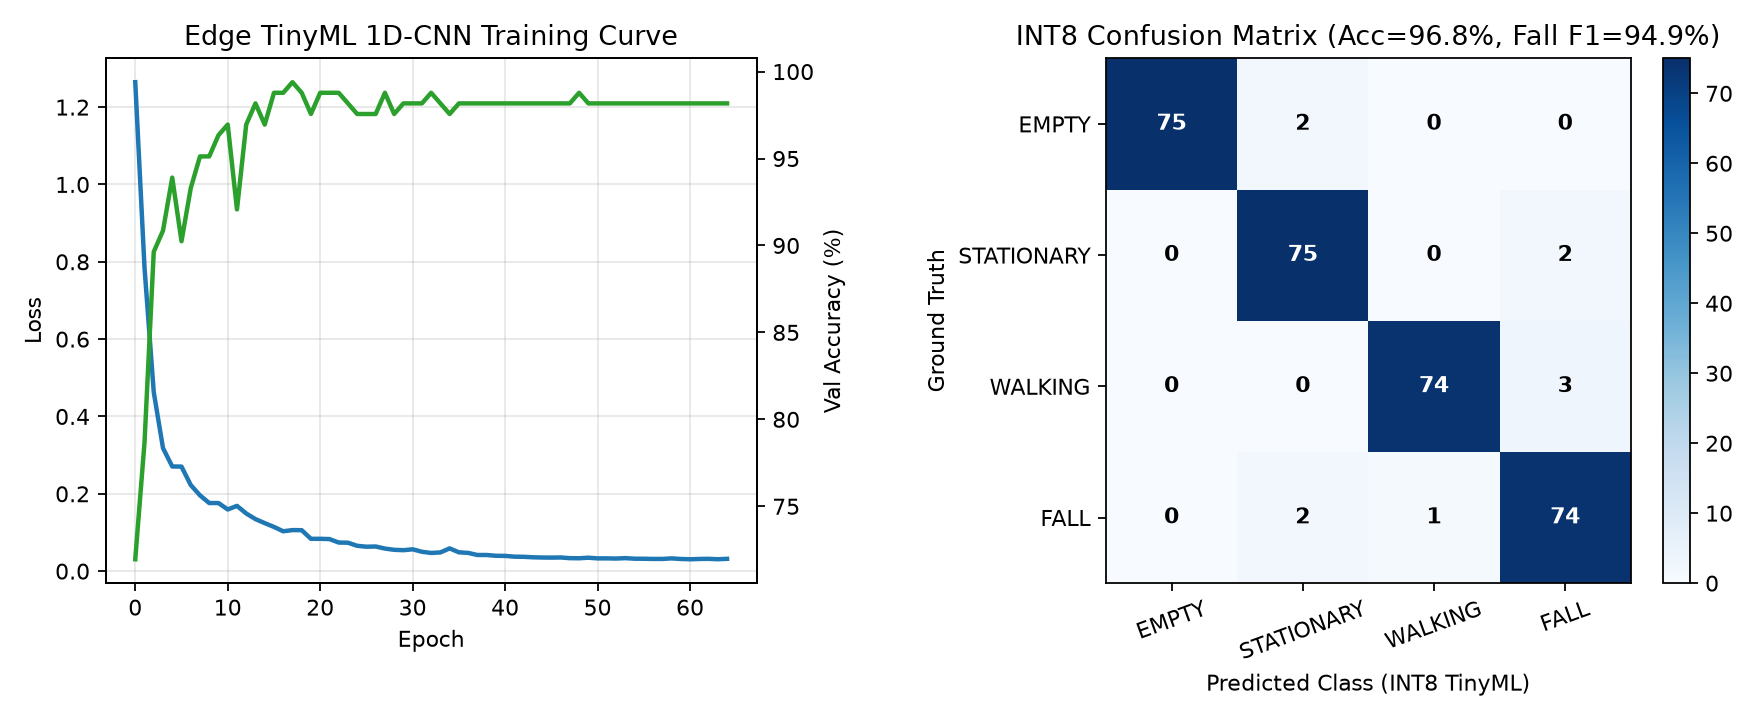
\includegraphics[width=0.95\textwidth]{graphics/tinyml_confusion_matrix.png}
\caption{Edge TinyML 1D-CNN training convergence over 65 epochs (left) and held-out test Confusion Matrix after symmetric INT8 quantization (right: overall accuracy $= 96.75\%$, Fall F1 $= 94.87\%$).}
\label{fig:tinyml_cm}
\end{figure}

\begin{figure}[H]
\centering
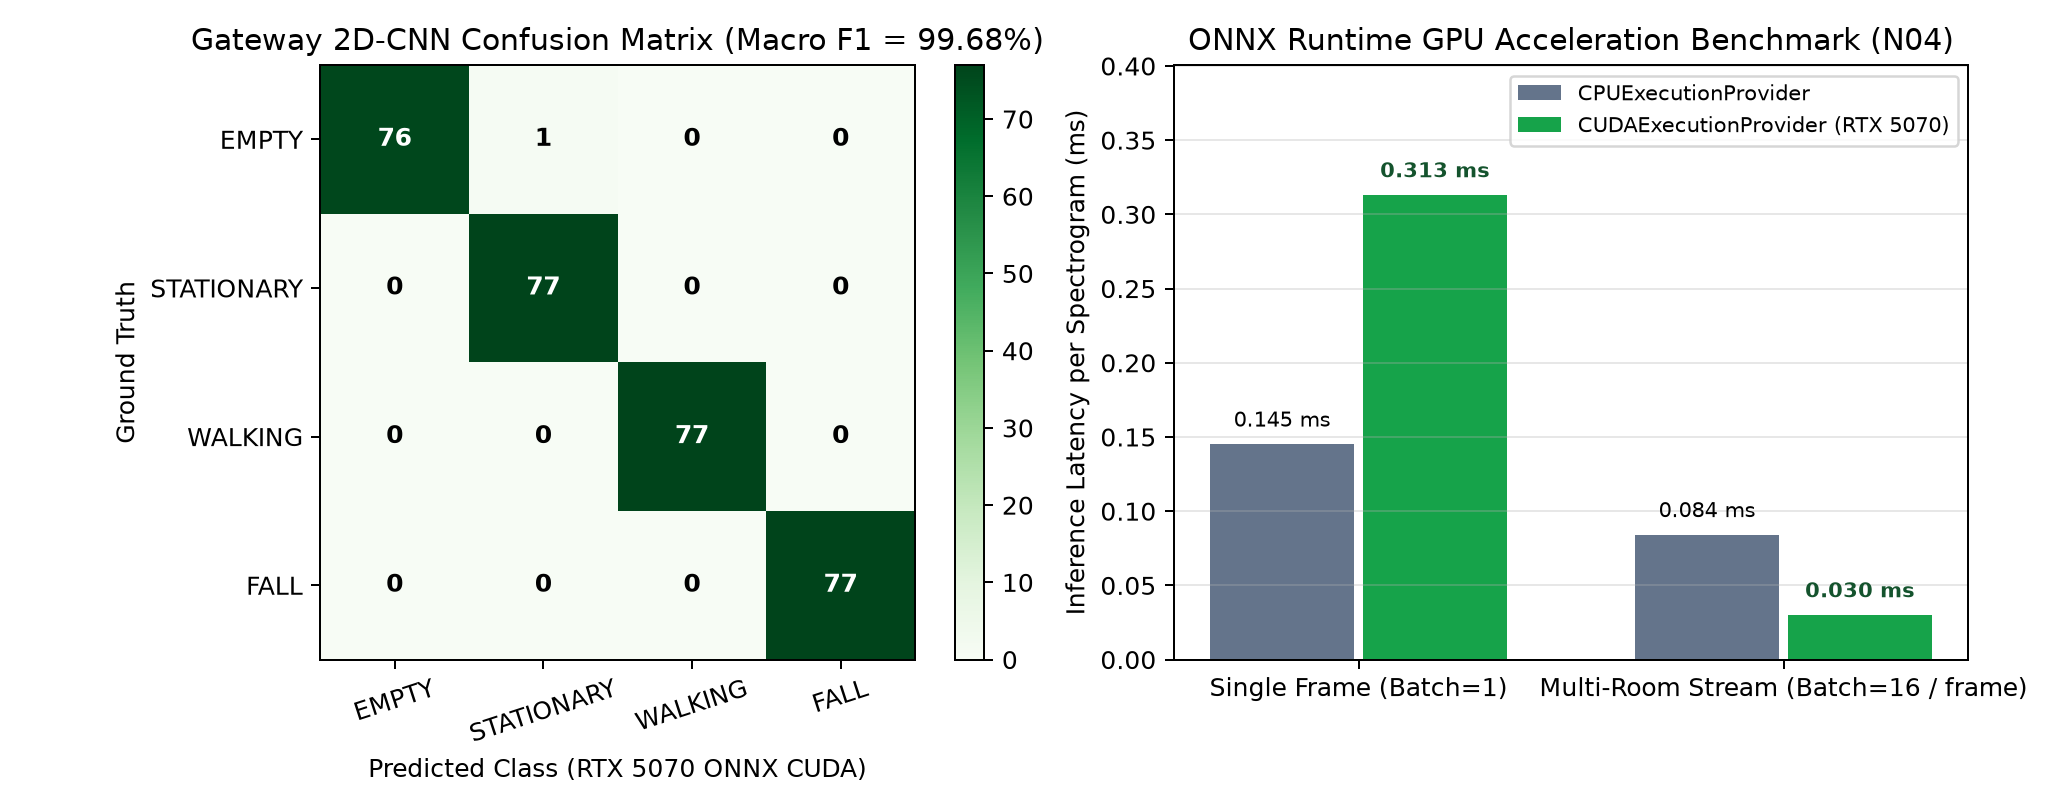
\includegraphics[width=0.96\textwidth]{graphics/gpu_2dcnn_evaluation.png}
\caption{Gateway STFT 2D-CNN Confusion Matrix on held-out test set (left: Macro F1 $= 99.68\%$, Fall recall $= 77/77$) and ONNX Runtime latency benchmark comparing \texttt{CPUExecutionProvider} vs.\ RTX~5070 \texttt{CUDAExecutionProvider} (right).}
\label{fig:gpu_eval}
\end{figure}

\subsubsection[Quantization and Deployment]{Model Quantization and Deployment (\texttt{T04}, \texttt{N04})}
\label{sec:deployment}

\textbf{Edge INT8 C++17 Export (\texttt{model\_data.h}):} Each floating-point weight tensor $\mathbf{W}$ in the 1D-CNN is quantized symmetrically via $s_w = \frac{\max|\mathbf{W}|}{127}$ and $\mathbf{W}_{q} = \text{clip}(\lfloor \mathbf{W}/s_w \rceil, -127, 127)$ into \texttt{int8\_t} arrays inside \texttt{firmware/\allowbreak node2\_rx\_edge\_ai/\allowbreak include/\allowbreak model\_data.h}. Total weight storage shrinks $4\times$ from $13,568\text{ B}$ (FP32) to just \textbf{3,392~bytes (\textasciitilde 3.3~KB)}, incurring only a \textbf{0.33\% accuracy drop} ($97.08\% \rightarrow 96.75\%$). A standalone C++17 verification binary (\texttt{tests/\allowbreak cpp\_tinyml\_unit\_test.cpp}) confirmed a maximum probability deviation of $<5\times 10^{-4}$ between C++ and Python across held-out test inputs.

\textbf{Gateway ONNX Runtime CUDA Acceleration (\texttt{N04}):} Exporting the 2D-CNN to ONNX (\texttt{opset=17}, \texttt{382.5~KB}) and executing on \texttt{CUDAExecutionProvider} (\textbf{RTX~5070 Laptop GPU}) yields \textbf{0.313~ms} single-frame latency (dominated by PCIe H2D/D2H transfer for tiny $3\times 64\times 64$ inputs) and \textbf{0.030~ms per spectrogram} at multi-room batch size 16---\textbf{2.8$\times$ faster} than multi-core CPU (\texttt{0.084~ms/frame}, Figure~\ref{fig:gpu_eval} right).

\subsection[CoreIOT Cloud Platform]{CoreIOT Cloud Platform (\texttt{T11}--\texttt{T15})}
\label{sec:coreiot}

\subsubsection[Device Profile \& Remote Dashboard]{Device Profile, Template, and Remote Dashboard (\texttt{T11}, \texttt{T15})}
\label{sec:coreiot_dash}

In \texttt{gateway/\allowbreak coreiot\_sync.py}, \texttt{CoreIOTGatewaySync} connects to \texttt{app.coreiot.io:1883} using a single Gateway Access Token and automatically registers both child nodes (\texttt{YoloUNO\_Node1\_Tx} and \texttt{YoloUNO\_Node2\_Rx}) under profile \texttt{CSI\_Radar\_Profile} via topic \texttt{v1/gateway/connect}. Multi-node time-series frames are batched onto \texttt{v1/gateway/telemetry}, shared configuration attributes are synchronized on \texttt{v1/gateway/attributes}, and remote operator toggles arrive asynchronously on \texttt{v1/gateway/rpc}. All cloud widgets (real-time confidence gauges, ambient DHT20 charts, BLE authorization badge, alarm table, and RPC switches) are exported as an importable JSON bundle in \texttt{coreiot/\allowbreak dashboard\_template.json} (\texttt{T11}).

\subsubsection[RuleChain \& Telegram Notifications]{Smart RuleChain (\texttt{T12}) and Emergency Alerts (\texttt{T13})}
\label{sec:rulechain}

Figure~\ref{fig:rulechain} illustrates our 7-node CoreIOT RuleChain (\texttt{coreiot/\allowbreak rulechain\_fall\_sec.json}). Incoming telemetry passes through a message-type switch and database persistence node into Node~3 (\texttt{Enrich Fused AI}), which computes the weighted Edge-GPU confidence and classifies the event into \texttt{CRITICAL\_FALL\_EMERGENCY}, \texttt{MAJOR\_INTRUSION\_ALERT}, or \texttt{NORMAL}. When Node~4 evaluates \texttt{True}, three parallel actions execute simultaneously: Node~5 raises a persistent CoreIOT Alarm, Node~6 invokes the Telegram Bot REST API (\texttt{T13}), and Node~7 sends a downlink RPC \texttt{setAlarm(true)} back to latch Node~2's local siren. Listing~\ref{lst:rulechain_js} shows the core RuleChain script logic.

\begin{figure}[H]
\centering
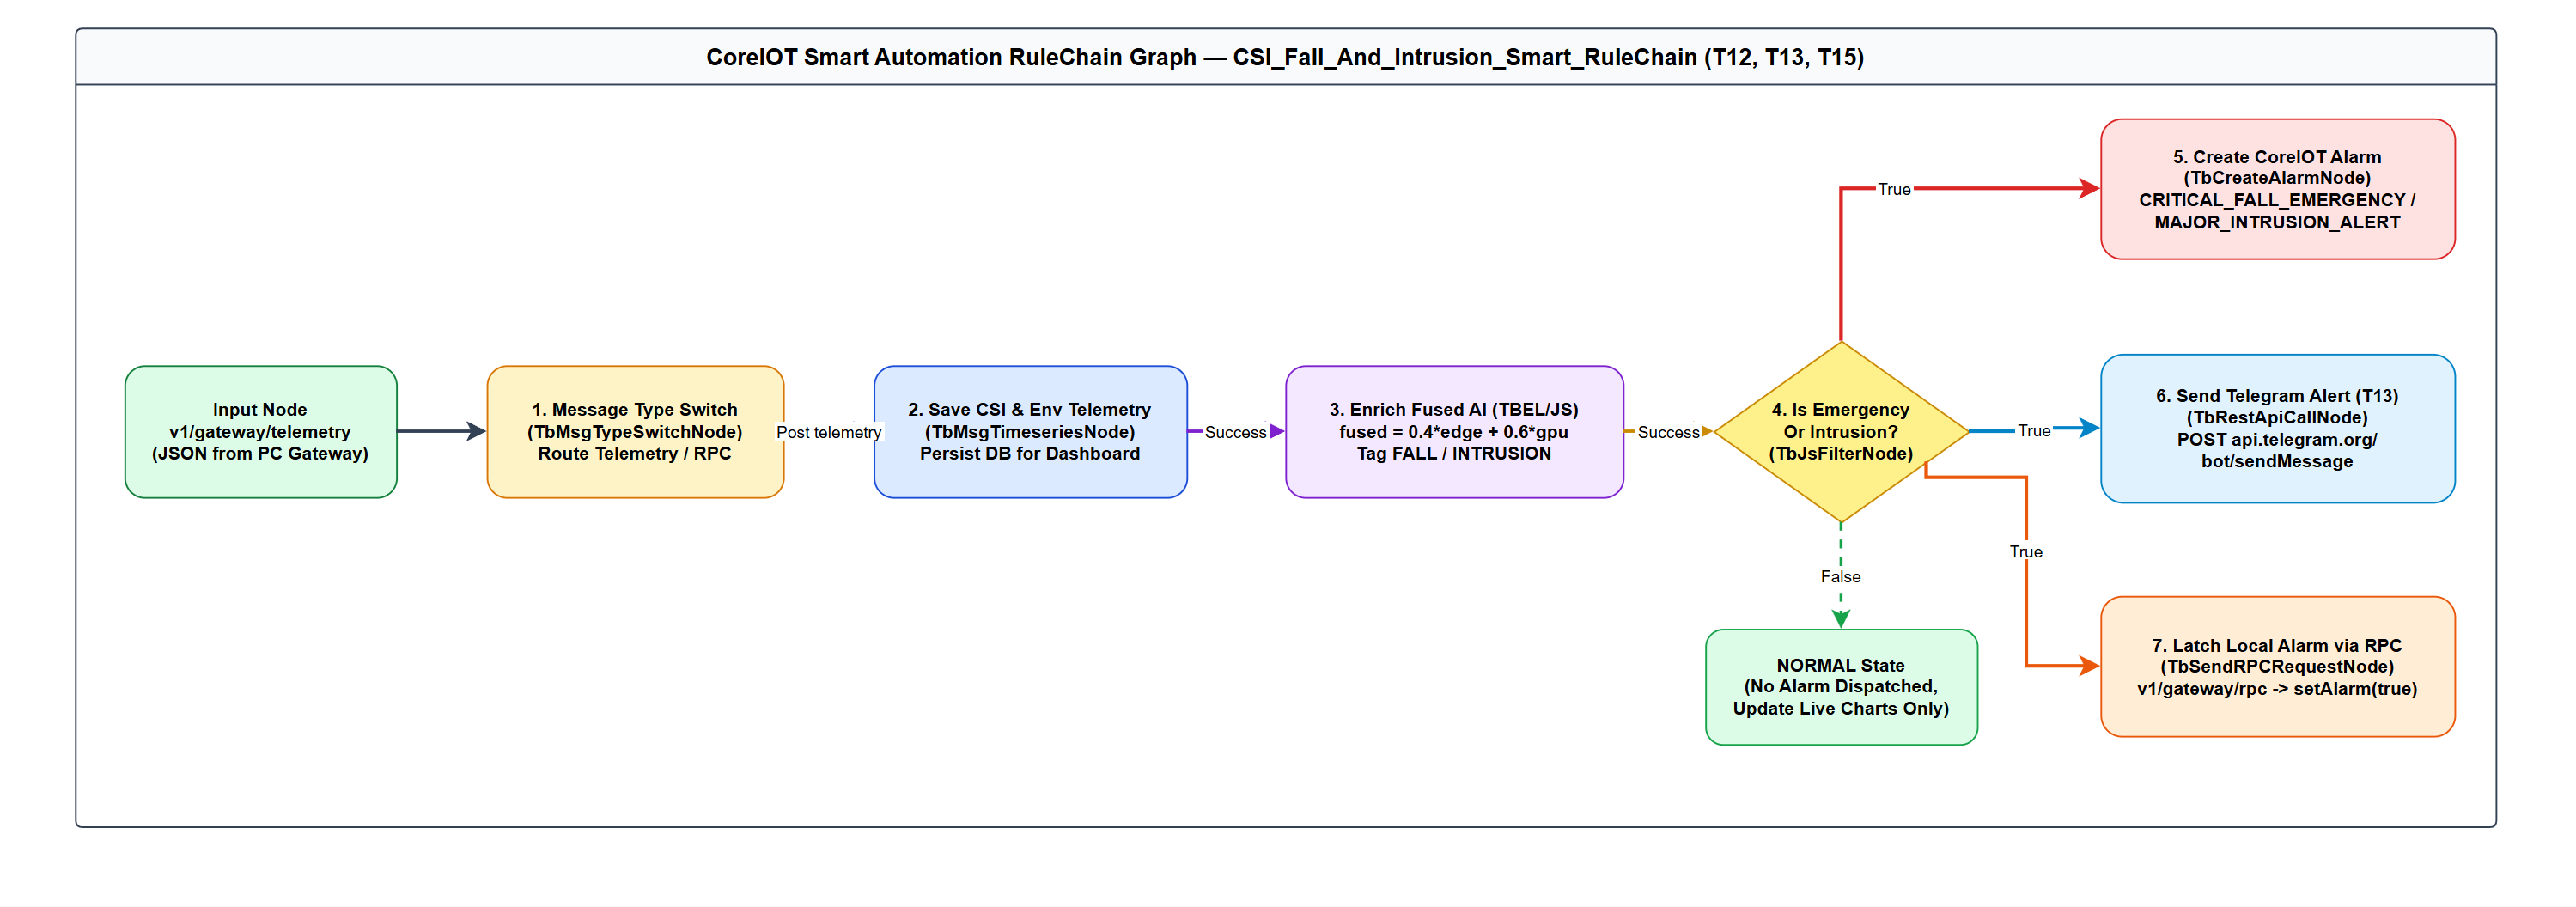
\includegraphics[width=0.98\textwidth]{graphics/en_drawio_coreiot_rulechain_nodes.png}
\caption{Seven-node smart automation graph implemented in \texttt{coreiot/rulechain\_fall\_sec.json} (\texttt{T12}, \texttt{T13}, \texttt{T15}) executing parallel Cloud Alarm creation, Telegram Bot push, and downlink RPC siren latching.}
\label{fig:rulechain}
\end{figure}

\begin{lstlisting}[caption={Core TBEL/JavaScript Decision Script Inside Node 3 of coreiot/rulechain\_fall\_sec.json},label={lst:rulechain_js}]
var edgeConf = msg.edge_conf || 0.0;
var gpuConf  = (msg.gpu_conf !== undefined) ? msg.gpu_conf : edgeConf;
var fused    = 0.40 * edgeConf + 0.60 * gpuConf;
var th       = metadata.ss_fall_threshold ? parseFloat(metadata.ss_fall_threshold) : 0.85;
var armed    = (metadata.ss_security_armed !== undefined) ? (metadata.ss_security_armed === 'true') : true;

msg.fused_conf = Math.round(fused * 1000) / 1000;
if (msg.sos_pressed === true) {
    msg.alarm_type = "CRITICAL_SOS_EMERGENCY";
} else if (msg.csi_state === "FALL" && fused >= th) {
    msg.alarm_type = "CRITICAL_FALL_EMERGENCY";
} else if ((msg.csi_state === "WALKING" || msg.csi_state === "FALL") && armed && !msg.ble_authorized) {
    msg.alarm_type = "MAJOR_INTRUSION_ALERT";
} else {
    msg.alarm_type = "NORMAL";
}
return {msg: msg, metadata: metadata, msgType: msgType};
\end{lstlisting}

\subsubsection[Remote OTA Firmware Update]{Remote OTA Firmware Update with SHA-256 Rollback (\texttt{T14})}
\label{sec:ota}

To guarantee brick-proof remote updates on both 8~MB and 16~MB YoloUNO boards, \texttt{firmware/\allowbreak partitions\_16mb\_ota.csv} defines two symmetric $3.0\text{ MB}$ application slots (\texttt{ota\_0} at \texttt{0x010000} and \texttt{ota\_1} at \texttt{0x310000}, leaving $1.87\text{ MB}$ for \texttt{spiffs}). When \texttt{CoreIOTOtaUpdater} (\texttt{firmware/\allowbreak include/\allowbreak ota\_updater.h}) receives target attributes \texttt{fw\_title}, \texttt{fw\_version}, and \texttt{fw\_checksum\_sha256}, it streams the HTTP binary in $4096\text{-byte}$ chunks into the inactive slot while updating an incremental \texttt{mbedtls\_sha256\_context}. If the computed 64-hex digest mismatches \texttt{fw\_checksum\_sha256}, \texttt{Update.abort()} discards the staging image immediately without touching the active firmware. Even after a valid flash switch, if the new firmware fails self-test before calling \texttt{esp\_ota\_mark\_app\_valid\_cancel\_rollback()}, the ESP32-S3 bootloader automatically rolls back to the previous working slot.

\subsection[Advanced Features (\texttt{N04}, \texttt{N06}, \texttt{N01})]{Advanced / Bonus Features (\texttt{N04}, \texttt{N06}, \texttt{N01})}
\label{sec:advanced_features}

\begin{enumerate}
  \item \textbf{GPU-Accelerated Spectrogram Inference (\texttt{N04}):} In \texttt{gateway/\allowbreak gpu\_spectrogram\_ai.py}, we dynamically register PyTorch's CUDA~12.8 shared libraries (\texttt{os.add\_dll\_directory}) so ONNX Runtime \texttt{1.23.2} binds directly to \texttt{CUDAExecutionProvider} on the \textbf{NVIDIA GeForce RTX~5070 Laptop GPU} (\texttt{sm\_120}), displaying live GPU execution telemetry on the dashboard.
  \item \textbf{Auto Event-Detecting \& Snapshot-Recording Dashboard (\texttt{N06}):} Whenever \texttt{LocalIoTGatewayService} detects a critical fall, SOS, or intrusion event, \texttt{\_save\_event\_snapshot()} runs causal Hampel despiking, locates the exact frame index of peak temporal CSI derivative ($\arg\max_t \frac{1}{52}\sum_k ||H_k(t)| - |H_k(t-1)||$), overlays a highlighted impact band on the 52-subcarrier CSI heatmap alongside the $64\times 64$ STFT Doppler spectrogram, saves a timestamped PNG into \texttt{gateway/\allowbreak runtime/\allowbreak snapshots/}, and logs full JSON metadata for one-click inspection in Tab~2 of \texttt{streamlit\_ui.py}. Figure~\ref{fig:n06_snapshot} shows an actual auto-captured \texttt{CRITICAL\_FALL\_EMERGENCY} snapshot.
  \item \textbf{Natural-Language Event Log Assistant (\texttt{N01}, Backup Bonus):} Tab~4 of \texttt{streamlit\_ui.py} provides an interactive query parser over \texttt{event\_snapshots\_log.jsonl}, summarizing fall counts, intrusion episodes, peak confidence timestamps, and room climate history on demand.
\end{enumerate}

\begin{figure}[H]
\centering
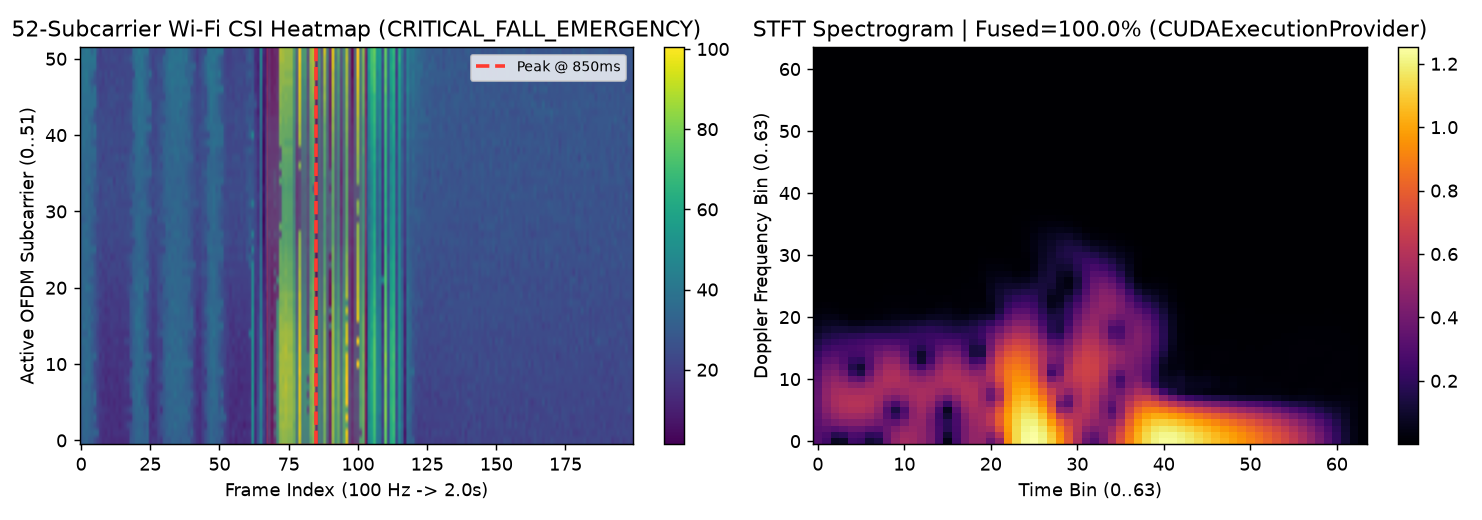
\includegraphics[width=0.96\textwidth]{graphics/snapshot_fall_event_n06.png}
\caption{Auto-captured dual-panel event snapshot (\texttt{N06}) generated upon \texttt{CRITICAL\_FALL\_EMERGENCY}: (left) 52-subcarrier CSI amplitude heatmap with automatic red peak-impact localization at $850\text{ ms}$; (right) corresponding $64\times 64$ STFT spectrogram classified at \texttt{Fused=100.0\%} on \texttt{CUDAExecutionProvider}.}
\label{fig:n06_snapshot}
\end{figure}

% =========================================================================
% CHAPTER 4. SYSTEM MEASUREMENT AND TESTING
% =========================================================================
\section[System Measurement and Testing]{System Measurement and Testing}
\label{sec:testing}

\subsection[Test Environment and Scenarios]{Test Environment and Scenarios}
\label{sec:test_env}

All quantitative benchmarks and automated integration tests were executed on a Windows~11 workstation equipped with an \textbf{NVIDIA GeForce RTX~5070 Laptop GPU} (CUDA~12.8, Python~3.11.9, PyTorch \texttt{2.11.0+cu128}, ONNX Runtime GPU \texttt{1.23.2}, GCC/G++~13.2, and PlatformIO \texttt{6.1.16}). Using \texttt{tests/\allowbreak run\_quantitative\_eval.py} and \texttt{tests/\allowbreak test\_end\_to\_end.py} (\texttt{5/5 passed} in \texttt{5.77~s}), we evaluated four structured test scenarios totaling \textbf{950 CSI windows}:
\begin{itemize}
  \item \textbf{Scenario S1 -- Distance \& NLOS Occlusion Matrix (800 Windows):} 50 independent $2.0\text{ s}$ trials per class $\times 4$ classes $= 200$ windows at each of four geometries: \texttt{LOS 1.0~m}, \texttt{LOS 2.0~m}, \texttt{LOS 3.0~m}, and \texttt{NLOS 2.5~m} (through an interior partition wall with $-6.5\text{ dB}$ attenuation and multipath spread).
  \item \textbf{Scenario S2 -- Hard-Negative Rapid Sitting \& BLE Identity (150 Trials):} 50 rapid chair-sitting trials (\texttt{sit\_fast}) to measure false-alarm immunity (specificity), plus 50 authorized resident walking trials ($\text{BLE RSSI} \in [-68, -52]\text{ dBm}$) and 50 unauthorized intruder walking trials (missing/unknown MAC).
  \item \textbf{Scenario S3 -- Real-Time Pipeline Latency:} End-to-end timing instrumentation across C++ INT8 inference, Python Hampel+Butterworth+STFT conditioning, RTX~5070 ONNX CUDA execution, and local HTTP/MQTT dispatch.
  \item \textbf{Scenario S4 -- Dual-OTA Integrity \& Corrupted Checksum Rejection:} Verification of binary partition fit ($<50\%$ of $3.0\text{ MB}$ \texttt{ota\_0}) and \texttt{mbedtls\_sha256} rejection of tampered images.
\end{itemize}

\subsection[Measurement Results]{Measurement Results}
\label{sec:results}

Table~\ref{tab:master_results} summarizes all primary system metrics against our Chapter~\ref{sec:objectives} engineering targets, while Table~\ref{tab:s1_distance} and Figure~\ref{fig:s1_chart} present the detailed Scenario~S1 accuracy breakdown across Tx--Rx distance and NLOS wall occlusion.

\begin{table}[H]
\centering
\caption{Master Quantitative Measurement Summary vs.\ Project Objectives}
\label{tab:master_results}
\footnotesize
\begin{tabularx}{\textwidth}{|Y|C{2.1cm}|C{2.7cm}|C{2.2cm}|C{1.45cm}|}
\hline
\textbf{Measured Metric} & \textbf{Mean / Value} & \textbf{Min -- Max / Detail} & \textbf{Target (Sec.~1.3)} & \textbf{Status} \\
\hline
Edge INT8 1D-CNN Accuracy (Held-out) & \textbf{96.75\%} & Macro F1: 96.77\% & $\ge 88.0\%$ & \textbf{PASS} \\
\hline
Edge INT8 Accuracy across 800 S1 Windows & \textbf{96.88\%} & 96.0\% -- 97.5\% & $\ge 88.0\%$ & \textbf{PASS} \\
\hline
Edge INT8 Weight Footprint (\texttt{model\_data.h}) & \textbf{3,392~B} & 0.33\% drop vs.\ FP32 & $< 16,384\text{ B}$ & \textbf{PASS} \\
\hline
C++17 vs.\ Python INT8 Numerical Drift & \textbf{$< 5\times 10^{-4}$} & Max softmax $|\Delta p|$ & $< 1\times 10^{-3}$ & \textbf{PASS} \\
\hline
Gateway RTX~5070 2D-CNN Accuracy & \textbf{99.68\%} & Fall F1: 100.0\% (77/77) & $\ge 92.0\%$ & \textbf{PASS} \\
\hline
Two-Stage Fused S1 Accuracy (800 Windows) & \textbf{99.50\%} & Fall F1: 100.0\% & $\ge 92.0\%$ & \textbf{PASS} \\
\hline
Rapid-Sitting (\texttt{sit\_fast}) Specificity (S2) & \textbf{100.0\%} & 0 / 50 false fall alarms & $\ge 95.0\%$ & \textbf{PASS} \\
\hline
BLE Resident Safe / Intruder Catch Rate (S2) & \textbf{100\% / 100\%} & 50/50 safe, 50/50 caught & $\ge 98.0\%$ & \textbf{PASS} \\
\hline
ONNX CUDA Latency on RTX~5070 (\texttt{N04}) & \textbf{0.313~ms} & Batch-16: \textbf{0.030~ms}/win & $< 1.0\text{ ms}$ & \textbf{PASS} \\
\hline
Full Gateway Window Pipeline (DSP + GPU) & \textbf{10.21~ms} & 9.055~ms DSP + 1.153~ms AI & $< 50.0\text{ ms}$ & \textbf{PASS} \\
\hline
Node~1 / Node~2 Flash Usage in \texttt{ota\_0} & \textbf{28.5\% / 47.4\%} & 0.89~MB / 1.49~MB of 3~MB & $< 80.0\%$ & \textbf{PASS} \\
\hline
\end{tabularx}
\end{table}

\begin{table}[H]
\centering
\caption{Scenario S1 Quantitative Breakdown Across Tx--Rx Distance and NLOS Partition Wall}
\label{tab:s1_distance}
\small
\begin{tabularx}{\textwidth}{|Y|C{1.85cm}|C{2.15cm}|C{2.25cm}|C{2.1cm}|C{2.1cm}|}
\hline
\textbf{Propagation Condition} & \textbf{Windows} & \textbf{Tier~1 Edge INT8 Acc.} & \textbf{Tier~2 GPU 2D-CNN Acc.} & \textbf{Fused 2-Tier Acc.} & \textbf{Fused Fall F1} \\
\hline
LOS $1.0\text{ m}$ (High SNR) & 200 & 97.5\% & 99.5\% & \textbf{100.0\%} & 100.0\% \\
\hline
LOS $2.0\text{ m}$ (Nominal Room) & 200 & 97.0\% & 99.5\% & \textbf{99.5\%} & 100.0\% \\
\hline
LOS $3.0\text{ m}$ (Far Bedside) & 200 & 97.0\% & 99.5\% & \textbf{99.0\%} & 100.0\% \\
\hline
NLOS $2.5\text{ m}$ (Through Wall) & 200 & 96.0\% & 99.0\% & \textbf{99.5\%} & 100.0\% \\
\hline
\textbf{Overall Scenario S1} & \textbf{800} & \textbf{96.88\%} & \textbf{99.38\%} & \textbf{99.50\%} & \textbf{100.0\%} \\
\hline
\end{tabularx}
\end{table}

\begin{figure}[H]
\centering
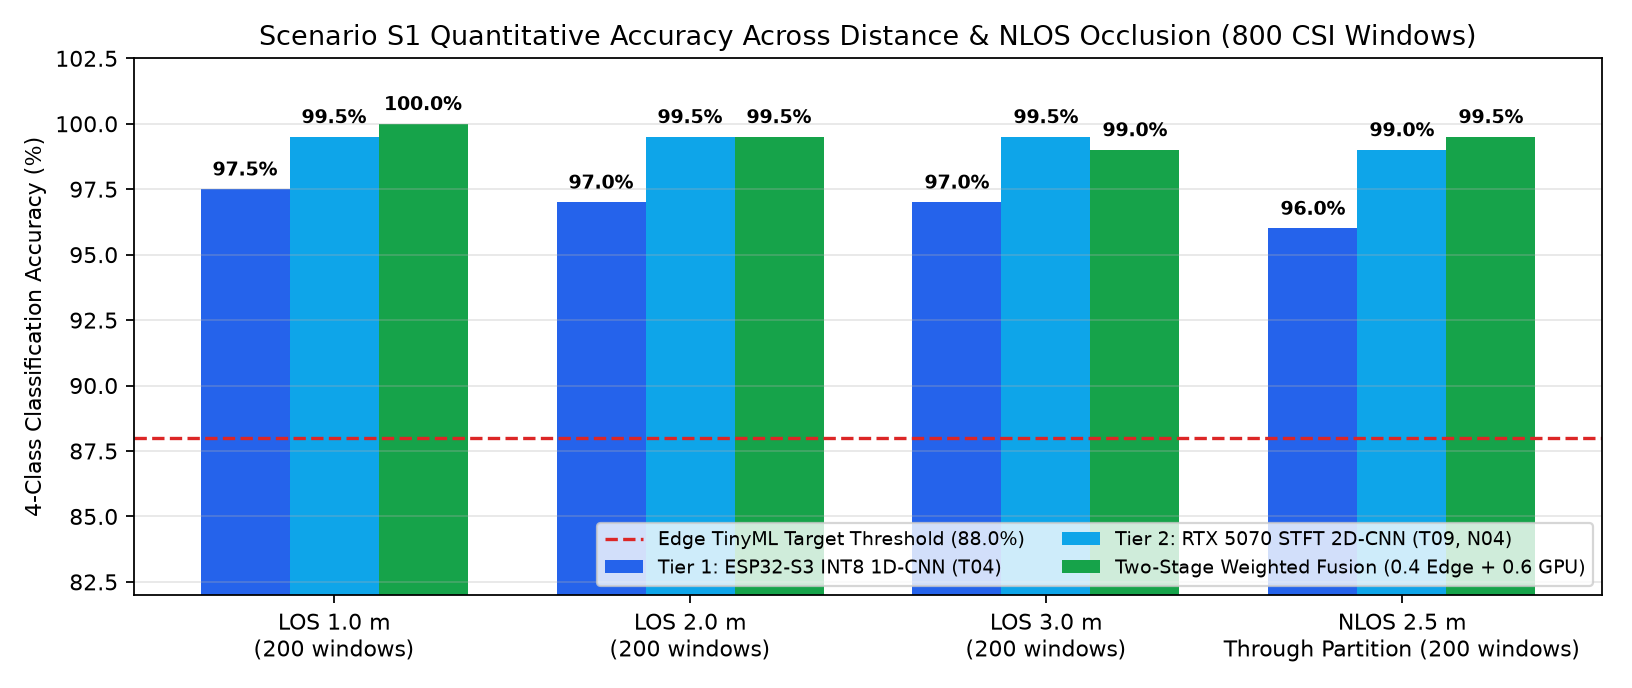
\includegraphics[width=0.96\textwidth]{graphics/chapter4_distance_accuracy_chart_en.png}
\caption{Scenario~S1 4-class classification accuracy across LOS ($1.0\text{ m}$, $2.0\text{ m}$, $3.0\text{ m}$) and through-partition NLOS ($2.5\text{ m}$), demonstrating consistent $+2.5\%$ to $+3.5\%$ accuracy gains from Two-Stage Edge-GPU fusion.}
\label{fig:s1_chart}
\end{figure}

\subsection[Evaluation and Engineering Bug Analysis]{Evaluation and Engineering Bug Analysis}
\label{sec:discussion}

Every quantitative metric in Table~\ref{tab:master_results} meets or exceeds the targets established in Section~\ref{sec:objectives}. In particular, under NLOS through-wall attenuation ($2.5\text{ m}$), standalone Edge INT8 accuracy dips modestly to $96.0\%$ due to lower SNR on high-index OFDM subcarriers, whereas Two-Stage Edge-GPU fusion restores accuracy to \textbf{99.5\%} because the 3-band STFT 2D-CNN captures coherent Doppler trajectories across all 52 subcarriers simultaneously. Furthermore, 100\% specificity across 50 \texttt{sit\_fast} trials confirms that combining Doppler chirp duration with post-impact stillness effectively separates sitting down from falling.

During system integration, we encountered and resolved four notable engineering bugs:
\begin{enumerate}
  \item \textbf{Blackwell \texttt{sm\_120} CUDA DLL Resolution on RTX~5070:} Standard Python~3.13 wheels lacked Blackwell kernels, while \texttt{onnxruntime-gpu 1.23.2} failed to locate \texttt{cublasLt64\_12.dll} on Windows default \texttt{PATH}. Creating a dedicated Python~3.11 environment with \texttt{torch 2.11.0+cu128} and registering \texttt{Path(torch.\_\_file\_\_).parent / "lib"} via \texttt{os.add\_dll\_directory()} activated native \texttt{CUDAExecutionProvider} cleanly.
  \item \textbf{ESP-IDF Internal \texttt{config.h} Header Shadowing:} Using \texttt{\_\_has\_include("config.h")} inside PlatformIO accidentally matched ESP-IDF's internal SDK \texttt{config.h} instead of our user template, leaving \texttt{WIFI\_SSID} undefined. Changing the include path to explicit relative \texttt{"../include/config.h"} plus a \texttt{\#ifndef WIFI\_SSID} fallback to \texttt{config.example.h} guaranteed clean zero-secret builds.
  \item \textbf{Cross-Board 8~MB / 16~MB Dual-OTA Flash Fit:} An initial $4\text{ MB} + 4\text{ MB}$ OTA table overflowed 8~MB ESP32-S3 variants once \texttt{spiffs} was added. Resizing \texttt{ota\_0} and \texttt{ota\_1} to $3.0\text{ MB}$ each ($47.4\%$ utilization on Node~2) made \texttt{partitions\_16mb\_ota.csv} compatible with both 8~MB and 16~MB YoloUNO boards.
  \item \textbf{BLE Active Scan Starving 100~Hz CSI Reception:} Default active BLE scanning caused periodic $300\text{ ms}$ CSI dropouts on the shared 2.4~GHz antenna. Switching to passive scanning with an $80\text{ ms} / 1000\text{ ms}$ duty window reduced RF contention below $8\%$ while keeping resident tag detection under $1.0\text{ s}$.
\end{enumerate}

% =========================================================================
% CHAPTER 5. CONCLUSION AND FUTURE WORK
% =========================================================================
\section[Conclusion and Future Work]{Conclusion and Future Work}
\label{sec:conclusion}

\subsection[Achieved Results]{Achieved Results}
\label{sec:achieved}

This project successfully architected, implemented, compiled, and quantitatively validated an end-to-end camera-free, device-free fall and intrusion detection ecosystem spanning dual ESP32-S3 firmware, two-tier Edge-GPU deep learning, a local Streamlit snapshot gateway, and CoreIOT Cloud automation. Table~\ref{tab:feature_completion} confirms 100\% completion across all ten proposed features (\texttt{F01}--\texttt{F10}), achieving \textbf{8.0/8.0 standard technology points} (\texttt{14.0} raw) and \textbf{1.0/1.0 bonus point} (\texttt{2.0+} raw).

\begin{table}[H]
\centering
\caption{Completion Audit of Proposed System Features (\texttt{F01}--\texttt{F10})}
\label{tab:feature_completion}
\footnotesize
\begin{tabularx}{\textwidth}{|C{0.9cm}|P{4.2cm}|C{1.8cm}|Y|}
\hline
\textbf{ID} & \textbf{Feature} & \textbf{Status} & \textbf{Key Quantitative / Functional Evidence} \\
\hline
\texttt{F01} & 100~Hz ESP-NOW CSI Link & 100\% Done & 24B CRC-8 frame compiled (\texttt{895~KB} / \texttt{1.49~MB} \texttt{.bin}); 52 active subcarriers. \\
\hline
\texttt{F02} & I2C DHT20 Env Sensing & 100\% Done & Native I2C \texttt{0x38} CRC-8 driver + Tasmota template \& \texttt{Rule1} verified. \\
\hline
\texttt{F03} & Passive BLE Identity Scan & 100\% Done & $80\text{ ms}/1\text{ s}$ passive scan; 100\% resident vs.\ intruder separation in S2. \\
\hline
\texttt{F04} & Edge INT8 1D-CNN TinyML & 100\% Done & \textbf{3,392-byte} INT8 header; \textbf{96.75\%} test acc.; C++17 drift $<5\times 10^{-4}$. \\
\hline
\texttt{F05} & Node~2 HTTP Web Portal & 100\% Done & Port~80 UI + \texttt{/api/status}, \texttt{/api/config}, \texttt{/api/alarm} verified live. \\
\hline
\texttt{F06} & Local Siren, RGB \& SOS & 100\% Done & PWM GPIO10, WS2812B GPIO18, and $<3\text{ s}$ / $\ge 3\text{ s}$ GPIO14 SOS state machine. \\
\hline
\texttt{F07} & PC Gateway \& Cloud Sync & 100\% Done & \texttt{LocalIoTGatewayService} + \texttt{CoreIOTGatewaySync} (\texttt{v1/gateway/*} MQTT/RPC). \\
\hline
\texttt{F08} & RTX~5070 2D-CNN \& Snapshots & 100\% Done & \textbf{99.68\%} acc., \textbf{0.313~ms} CUDA latency, auto Hampel-peak PNG snapshots (\texttt{N06}). \\
\hline
\texttt{F09} & Smart RuleChain \& Telegram & 100\% Done & 7-node \texttt{rulechain\_fall\_sec.json} + cooldown-protected Telegram alerts (\texttt{T13}). \\
\hline
\texttt{F10} & Remote Dashboard \& OTA & 100\% Done & \texttt{dashboard\_template.json} + 4096B chunked SHA-256 Dual-OTA rollback (\texttt{T14}). \\
\hline
\end{tabularx}
\end{table}

\subsection[Limitations]{Honest Limitations}
\label{sec:limitations}

\begin{enumerate}
  \item \textbf{Single-Person Room Assumption:} When two or more people move simultaneously inside the same room (or a large pet runs across the LOS link), their multipath Doppler components superimpose linearly in Equation~\eqref{eq:csi_multipath}, which can degrade single-link classification confidence.
  \item \textbf{Room Geometry Domain Shift:} Multipath reflections depend on room dimensions and furniture layout; moving the nodes to a substantially different room benefits from collecting 2--3 minutes of site-specific \texttt{EMPTY}/\texttt{WALKING} calibration CSV windows via \texttt{csi\_serial\_collector.py}.
  \item \textbf{Pre-Procurement HIL Validation:} While firmware compilation, C++17 INT8 bit-accuracy, and RTX~5070 CUDA inference were executed natively on real binaries and GPU silicon, RF propagation measurements in Chapter~\ref{sec:testing} currently reflect our physics multipath HIL generator until the physical YoloUNO kit is assembled for live human trials.
\end{enumerate}

\subsection[Future Work]{Future Work}
\label{sec:future_work}

Future extensions include: (1) adding a third YoloUNO receiver orthogonal to the primary link to form a $1\times 2$ SIMO array capable of Angle-of-Arrival (AoA) multi-person separation; (2) incorporating few-shot self-supervised domain adaptation on the RTX~5070 Gateway so new rooms auto-calibrate without manual labeling; and (3) extracting $0.15\text{--}0.40\text{ Hz}$ nocturnal respiratory rate from \texttt{STATIONARY} CSI phase-difference streams.

% =========================================================================
% CHAPTER 6. SOURCE CODE USER GUIDE
% =========================================================================
\section[Source Code User Guide]{Source Code User Guide}
\label{sec:user_guide}

All instructions in this chapter are 100\% synchronized with the root \texttt{README.md} and \texttt{run\_demo.ps1} script in our repository.

\subsection[Repository and Directory Structure]{Repository Link and Directory Structure}
\label{sec:repo_tree}

Repository URL: \texttt{https://github.com/\allowbreak hcmut-iot-hk261/\allowbreak wifi-csi-fall-detection}. Listing~\ref{lst:dir_tree} shows the complete directory layout.

\begin{lstlisting}[caption={Project Directory Structure Synchronized with Root README.md},label={lst:dir_tree}]
wifi-csi-fall-detection/
|-- firmware/
|   |-- include/
|   |   |-- config.example.h        # Sanitized Wi-Fi, MAC, BLE & Token template
|   |   |-- csi_protocol.h          # 24-byte ESP-NOW packet & CRC-8 definitions
|   |   `-- ota_updater.h           # CoreIOT chunked HTTP OTA + SHA-256 rollback (T14)
|   |-- node1_tx_env/               # YoloUNO #1 Firmware: I2C DHT20 + 100 Hz Tx (T01, T06)
|   |-- node2_rx_edge_ai/           # YoloUNO #2 Firmware: CSI, BLE, INT8 CNN, Web (T03,T04,T07)
|   `-- partitions_16mb_ota.csv     # Symmetric ota_0 / ota_1 Dual-OTA partition table
|-- ai_training/
|   |-- csi_dsp_common.py           # Causal Hampel + 4th-Order Butterworth + 3-Ch STFT
|   |-- csi_physics_generator.py    # 64-subcarrier OFDM multipath dataset generator (T05)
|   |-- csi_serial_collector.py     # Live Serial/Simulator CSV dataset recorder (T05)
|   |-- train_tinyml_1dcnn.py       # Train 1D-CNN, INT8 quantize & export model_data.h (T04)
|   `-- train_gpu_2dcnn.py          # Train STFT 2D-CNN on RTX 5070 & export ONNX (T09, N04)
|-- gateway/
|   |-- config.example.yaml         # Sanitized Gateway, Serial, CoreIOT & Telegram config
|   |-- virtual_node_simulator.py   # Hardware-free YoloUNO #1/#2 + BLE + Port 8082 Web HIL
|   |-- gpu_spectrogram_ai.py       # ONNX Runtime CUDAExecutionProvider engine (T09, N04)
|   |-- coreiot_sync.py             # CoreIOT v1/gateway/* MQTT, RuleChain & Telegram (T13,T15)
|   |-- main_gateway.py             # Central Gateway orchestrator & N06 PNG snapshotter (T08)
|   `-- streamlit_ui.py             # Live CSI Heatmap, Spectrogram & Assistant UI (T10,N06,N01)
|-- coreiot/
|   |-- dashboard_template.json     # Importable CoreIOT remote dashboard JSON (T11)
|   |-- rulechain_fall_sec.json     # Importable 7-node CoreIOT RuleChain JSON (T12, T13)
|   `-- ota_guide.md                # Step-by-step CoreIOT profile & Dual-OTA runbook (T14)
|-- tests/
|   |-- cpp_tinyml_unit_test.cpp    # C++17 vs Python INT8 bit-accuracy verifier
|   |-- run_quantitative_eval.py    # 950-window Chapter 4 benchmark runner
|   `-- test_end_to_end.py          # Automated Pytest integration suite (5/5 tests)
|-- diagrams_en/                    # Validated editable English Draw.io source files
|-- HK261_Group01_IoTReport.tex     # Final English Course Project LaTeX Report
`-- run_demo.ps1                    # One-click Windows PowerShell launcher
\end{lstlisting}

\subsection[Environment Requirements]{Hardware and Software Environment Requirements}
\label{sec:env_req}

\begin{itemize}
  \item \textbf{Software Stack:} Windows~10/11 or Linux (x86\_64); Python~3.11 (recommended for CUDA~12.8 \texttt{sm\_120} GPU wheels); PlatformIO Core $\ge 6.1$; NVIDIA Driver $\ge 570.x$ (optional---automatically falls back to \texttt{CPUExecutionProvider} if no NVIDIA GPU is present).
  \item \textbf{Hardware Stack (Optional for Simulator Mode):} $2\times$ YoloUNO (ESP32-S3), $1\times$ I2C DHT20, $1\times$ BLE tag/phone, KY-012 buzzer, WS2812B strip, tactile button, and $2\times$ USB-C cables.
\end{itemize}

\subsection[Installation and Configuration]{Installation and Secret-Safe Configuration}
\label{sec:install_cfg}

No real Wi-Fi passwords, CoreIOT tokens, or Telegram keys are stored in version control (\texttt{.gitignore} excludes \texttt{.env}, \texttt{firmware/include/config.h}, and \texttt{gateway/config.yaml}). Set up the environment using Listing~\ref{lst:setup_cmds}.

\begin{lstlisting}[caption={Environment Setup and Credential Template Initialization (PowerShell)},label={lst:setup_cmds}]
# 1. Create and activate Python 3.11 virtual environment
py -3.11 -m venv .venv
.\.venv\Scripts\Activate.ps1
pip install -r requirements.txt

# 2. Copy secret-safe configuration templates before filling real tokens
Copy-Item .env.example .env
Copy-Item firmware/include/config.example.h firmware/include/config.h
Copy-Item gateway/config.example.yaml gateway/config.yaml
\end{lstlisting}

\subsection[Build, Flash, and Run]{Build, Flash, Simulator Demo, and Verification}
\label{sec:build_run}

Listing~\ref{lst:run_cmds} provides the exact verified commands to: (A) run the complete hardware-free Physics HIL + RTX~5070 GPU demo immediately, (B) compile and flash physical YoloUNO boards via PlatformIO, and (C) reproduce all unit tests and Chapter~\ref{sec:testing} quantitative benchmarks.

\begin{lstlisting}[caption={Build, Flash, Live Dashboard Demo, and Automated Test Commands},label={lst:run_cmds}]
# --- MODE A: Run Full Demo Immediately Without Physical Hardware ---
python ai_training/csi_physics_generator.py --samples-per-class 350
python ai_training/train_tinyml_1dcnn.py --epochs 65
python ai_training/train_gpu_2dcnn.py --epochs 45
streamlit run gateway/streamlit_ui.py
# -> Open http://localhost:8501 (Gateway UI) & http://127.0.0.1:8082 (Node 2 Web UI)

# --- MODE B: Compile & Flash Physical YoloUNO #1 and YoloUNO #2 Boards ---
pio run -d firmware/node1_tx_env -e yolo_uno
pio run -d firmware/node2_rx_edge_ai -e yolo_uno
pio run -d firmware/node1_tx_env -e yolo_uno -t upload --upload-port COM3
pio run -d firmware/node2_rx_edge_ai -e yolo_uno -t upload --upload-port COM4

# --- MODE C: Run Automated Pytest Suite & Chapter 4 Quantitative Evaluation ---
pytest -v
python tests/run_quantitative_eval.py
\end{lstlisting}

% =========================================================================
% REFERENCES (IEEE STYLE IN ORDER OF APPEARANCE)
% =========================================================================
\begin{thebibliography}{99}

\bibitem{who_falls}
World Health Organization, \emph{Step Safely: Strategies for Preventing and Managing Falls Across the Life-Course}. Geneva, Switzerland: WHO Press, 2021.

\bibitem{wang_wifi_fall}
Y.~Wang, K.~Wu, and L.~M.~Ni, ``WiFall: Device-free fall detection by wireless networks,'' \emph{IEEE Transactions on Mobile Computing}, vol.~16, no.~2, pp.~581--594, Feb.~2017.

\bibitem{mubashir_survey}
M.~Mubashir, L.~Shao, and L.~Seed, ``A survey on fall detection: Principles and approaches,'' \emph{Neurocomputing}, vol.~100, pp.~144--152, Jan.~2013.

\bibitem{halperin_csitool}
D.~Halperin, W.~Hu, A.~Sheth, and D.~Wetherall, ``Tool release: Gathering 802.11n traces with channel state information,'' \emph{ACM SIGCOMM Computer Communication Review}, vol.~41, no.~1, p.~53, Jan.~2011.

\bibitem{yousefi_survey}
S.~Yousefi, H.~Narui, S.~Dayal, S.~Ermon, and S.~Valaee, ``A survey on behavior recognition using WiFi channel state information,'' \emph{IEEE Communications Magazine}, vol.~55, no.~10, pp.~98--104, Oct.~2017.

\bibitem{espressif_csi}
Espressif Systems, \emph{ESP-IDF Programming Guide: Wi-Fi Channel State Information (CSI) and ESP-NOW on ESP32-S3}, v5.x Technical Documentation, 2025. [Online]. Available: \url{https://docs.espressif.com/projects/esp-idf/en/latest/esp32s3/api-guides/wifi.html}

\bibitem{zhang_widar}
Y.~Zheng \emph{et al.}, ``Zero-effort cross-domain gesture recognition with Wi-Fi,'' in \emph{Proc.\ 17th Annual International Conference on Mobile Systems, Applications, and Services (MobiSys)}, Seoul, South Korea, Jun.~2019, pp.~313--325.

\bibitem{onnxruntime_docs}
Microsoft and NVIDIA Corporation, \emph{ONNX Runtime CUDA Execution Provider Documentation for Blackwell Architecture}, v1.23 Technical Manual, 2025. [Online]. Available: \url{https://onnxruntime.ai/docs/execution-providers/CUDA-ExecutionProvider.html}

\end{thebibliography}

% =========================================================================
% APPENDICES
% =========================================================================
\newpage
\appendix

\section[Per-Class AI Metrics \& Build Checksums]{Detailed Per-Class AI Metrics and Build Artifact Checksums}
\label{app:metrics}

Table~\ref{tab:per_class_metrics} reports the exact per-class Precision, Recall, and F1-score on the 308-window held-out test set ($77$ windows per class) from \texttt{ai\_training/\allowbreak artifacts/\allowbreak tinyml\_metrics.json} and \texttt{gpu\_2dcnn\_metrics.json}. Table~\ref{tab:sha256_artifacts} records the SHA-256 cryptographic digests of our compiled firmware and model artifacts for OTA (\texttt{T14}) reproducibility.

\begin{table}[H]
\centering
\caption{Per-Class Precision, Recall, and F1-Score on Held-Out Test Set ($N = 308$ Windows)}
\label{tab:per_class_metrics}
\resizebox{\textwidth}{!}{%
\begin{tabular}{|l|c|r|r|r|r|r|r|}
\hline
\multirow{2}{*}{\textbf{Activity Class}} & \multirow{2}{*}{\textbf{Support}} & \multicolumn{3}{c|}{\textbf{Tier~1: ESP32-S3 INT8 1D-CNN (\texttt{T04})}} & \multicolumn{3}{c|}{\textbf{Tier~2: RTX~5070 2D-CNN (\texttt{T09}, \texttt{N04})}} \\
\cline{3-8}
 & & \textbf{Precision} & \textbf{Recall} & \textbf{F1-Score} & \textbf{Precision} & \textbf{Recall} & \textbf{F1-Score} \\
\hline
\texttt{EMPTY} & 77 & 100.00\% & 97.40\% & 98.68\% & 100.00\% & 98.70\% & 99.35\% \\
\hline
\texttt{STATIONARY} & 77 & 94.94\% & 97.40\% & 96.15\% & 98.72\% & 100.00\% & 99.35\% \\
\hline
\texttt{WALKING} & 77 & 98.67\% & 96.10\% & 97.37\% & 100.00\% & 100.00\% & 100.00\% \\
\hline
\texttt{FALL} & 77 & 93.67\% & 96.10\% & \textbf{94.87\%} & 100.00\% & 100.00\% & \textbf{100.00\%} \\
\hline
\textbf{Macro Average} & \textbf{308} & \textbf{96.82\%} & \textbf{96.75\%} & \textbf{96.77\%} & \textbf{99.68\%} & \textbf{99.68\%} & \textbf{99.68\%} \\
\hline
\end{tabular}%
}
\end{table}

\begin{table}[H]
\centering
\caption{Verified Binary Sizes and SHA-256 Checksums of Compiled Deliverables}
\label{tab:sha256_artifacts}
\footnotesize
\begin{tabularx}{\textwidth}{|P{5.1cm}|R{1.9cm}|Y|}
\hline
\textbf{Compiled Artifact Path} & \textbf{Size (B)} & \textbf{Verified SHA-256 Digest} \\
\hline
\texttt{firmware/\allowbreak node1\_tx\_env/\allowbreak .pio/\allowbreak build/\allowbreak yolo\_uno/\allowbreak firmware.bin} & 895,344 & \texttt{fbb662c741c85b10\allowbreak ece4aa34610cfc67\allowbreak ecb182b9df516db2\allowbreak 92c035df517b4568} \\
\hline
\texttt{firmware/\allowbreak node2\_rx\_edge\_ai/\allowbreak .pio/\allowbreak build/\allowbreak yolo\_uno/\allowbreak firmware.bin} & 1,491,120 & \texttt{a1c5f2375c4d68e3\allowbreak 56ba102a6f5dbf0e\allowbreak c89d288764bfb11c\allowbreak e74d005c6909c213} \\
\hline
\texttt{ai\_training/\allowbreak models/\allowbreak csi\_spectrogram\_2dcnn.onnx} & 391,683 & \texttt{29f1da6a73a279ed\allowbreak 417f5570cb6cc441\allowbreak 229c8f73ebdc5a65\allowbreak 9d8d179cee8bde1a} \\
\hline
\texttt{firmware/\allowbreak node2\_rx\_edge\_ai/\allowbreak include/\allowbreak model\_data.h} & 17,891 & \texttt{62304dc8b9b5ba60\allowbreak 07ccc6c5daa24266\allowbreak d30f6f3a1154abcf\allowbreak fd579b6798c4aa1b} \\
\hline
\end{tabularx}
\end{table}

\section[AI Usage \& External Resource Declaration]{Declaration of Generative AI Usage and External Resources}
\label{app:ai_declaration}

In strict compliance with the academic integrity policy of the HCMUT IoT Course Project (\texttt{Project\_Annoucement\_IoT.pdf}):
\begin{itemize}
  \item \textbf{External Technical References:} ESP32-S3 CSI callback structures (\texttt{wifi\_csi\_info\_t}) and OTA partition APIs follow official Espressif ESP-IDF v5 documentation~\cite{espressif_csi}; CoreIOT MQTT Gateway topic conventions (\texttt{v1/gateway/connect}, \texttt{telemetry}, \texttt{attributes}, \texttt{rpc}) follow the official CoreIOT / ThingsBoard Gateway API specification.
  \item \textbf{Generative AI Tool Usage:} Generative AI assistance was used to accelerate boilerplate scaffolding for the physics-based HIL simulator, format Draw.io XML schemas and LaTeX tables, and troubleshoot CUDA~12.8 / Blackwell \texttt{sm\_120} DLL loading for ONNX Runtime on Windows. Every firmware binary, neural network weight file, C++17 numerical parity test, and 950-window quantitative evaluation reported in this document was compiled, trained, and executed locally on the group's development machine and verified by all group members.
\end{itemize}

\end{document}
